% Main entry point for the NABTA graduation project documentation.
% Compile locally with the "XeLaTeX + BibTeX" LaTeX Workshop recipe.

\documentclass[12pt,oneside,openany]{book}

% Package configuration for the NABTA report.
% Keep this file package-only; colours, layout, and commands live separately.

\usepackage{fontspec}
\usepackage{XCharter}
\usepackage[english]{babel}
\usepackage{csquotes}
\usepackage[a4paper,left=2cm,right=2cm,top=2cm,bottom=2cm,headheight=22pt,headsep=0.45cm,footskip=1.1cm]{geometry}
\usepackage{microtype}
\usepackage{setspace}
\usepackage{fancyhdr}
\usepackage{emptypage}
\usepackage[dvipsnames,svgnames,x11names,table]{xcolor}
\usepackage{graphicx}
\usepackage{float}
\usepackage{subcaption}
\usepackage{tikz}
\usepackage{pgfplots}
\pgfplotsset{compat=1.18}
\usetikzlibrary{arrows.meta,backgrounds,calc,fit,positioning,shapes.geometric,shapes.symbols}
\usepackage{booktabs}
\usepackage{longtable}
\usepackage{tabularx}
\usepackage{multirow}
\usepackage{array}
\usepackage{ragged2e}
\usepackage{makecell}
\usepackage{amsmath}
\usepackage{amssymb}
\usepackage{amsthm}
\usepackage{mathtools}
\usepackage{listings}
\usepackage[font=small,labelfont=bf,labelsep=period,margin=10pt,tableposition=top]{caption}
\usepackage{enumitem}
\usepackage{etoolbox}
\usepackage{titlesec}
\usepackage{titletoc}
\usepackage[acronym,toc,nonumberlist,nogroupskip,nopostdot]{glossaries}
\usepackage{pdfpages}
\usepackage{rotating}
\usepackage{pdflscape}
\usepackage{soul}
\usepackage[skins,breakable,listings]{tcolorbox}
\usepackage{datetime2}
\usepackage{xspace}
\usepackage[
  bookmarks=true,
  bookmarksnumbered=true,
  pdftitle={NABTA: Plant Disease Analysis System Using End-to-End Artificial Intelligence},
  pdfauthor={NABTA Graduation Project Team},
  pdfsubject={Graduation Project Report, Helwan University, 2026},
  pdfkeywords={plant disease, artificial intelligence, YOLOv8, U-Net, CNN, Grad-CAM, RAG, FastAPI}
]{hyperref}
\usepackage[nameinlink,capitalise,noabbrev]{cleveref}
\usepackage{bidi}

% Monochrome academic palette for a formal thesis presentation.

\definecolor{NabtaDark}{RGB}{0, 0, 0}
\definecolor{NabtaGold}{RGB}{0, 0, 0}
\definecolor{NabtaBlue}{RGB}{0, 0, 0}
\definecolor{NabtaGreen}{RGB}{0, 0, 0}
\definecolor{NabtaInk}{RGB}{0, 0, 0}
\definecolor{NabtaMuted}{RGB}{0, 0, 0}
\definecolor{NabtaSoft}{RGB}{255, 255, 255}
\definecolor{NabtaLine}{RGB}{0, 0, 0}
\definecolor{NabtaStripe}{RGB}{255, 255, 255}
\definecolor{LinkBlue}{RGB}{0, 0, 0}
\definecolor{CodeGray}{RGB}{255, 255, 255}
\definecolor{RuleGray}{RGB}{0, 0, 0}

% Global typography, page layout, headings, captions, tables, and code styling.

% XCharter closely matches the Charter BT typography used by the reference.
\defaultfontfeatures{Ligatures=TeX,Scale=MatchLowercase}

\setstretch{1.55}
\setlength{\parindent}{0pt}
\setlength{\parskip}{0.55em}
\setlength{\emergencystretch}{2em}

\pagestyle{fancy}
\fancyhf{}
\fancyhead[L]{\scriptsize\itshape\color{NabtaDark}\nouppercase{\leftmark}}
\fancyhead[R]{\scriptsize\bfseries\color{NabtaDark}\nabta}
\fancyfoot[C]{\scriptsize\color{NabtaDark}\thepage}
\renewcommand{\headrulewidth}{0.35pt}
\renewcommand{\footrulewidth}{0pt}
\renewcommand{\headrule}{\hbox to\headwidth{\color{black}\leaders\hrule height \headrulewidth\hfill}}

\fancypagestyle{plain}{%
  \fancyhf{}
  \fancyfoot[C]{\scriptsize\color{NabtaDark}\thepage}
  \renewcommand{\headrulewidth}{0pt}
}

\titleformat{\chapter}[display]
  {\normalfont\bfseries\color{NabtaDark}}
  {\vspace{-0.9cm}\small\color{NabtaGold}\MakeUppercase{\chaptertitlename}\ \thechapter}
  {0.55em}
  {\LARGE}
  [\vspace{1.15em}{\color{NabtaGold}\titlerule[0.8pt]}]
\titleformat{name=\chapter,numberless}[display]
  {\normalfont\bfseries\color{NabtaDark}}
  {\vspace{-0.9cm}}
  {0pt}
  {\LARGE}
  [\vspace{1.15em}{\color{NabtaGold}\titlerule[0.8pt]}]
\titlespacing*{\chapter}{0pt}{1pt}{40pt}
\titlespacing*{name=\chapter,numberless}{0pt}{-13pt}{30pt}

\titleformat{\section}
  {\normalfont\large\bfseries\color{NabtaDark}}
  {\thesection}{0.7em}{}
\titleformat{\subsection}
  {\normalfont\normalsize\bfseries\color{NabtaDark}}
  {\thesubsection}{0.7em}{}
\titleformat{\subsubsection}
  {\normalfont\normalsize\bfseries\color{NabtaDark}}
  {\thesubsubsection}{0.7em}{}
\titlespacing*{\section}{0pt}{1.8em}{0.8em}
\titlespacing*{\subsection}{0pt}{1.45em}{0.55em}
\titlespacing*{\subsubsection}{0pt}{1.2em}{0.45em}

\setcounter{tocdepth}{3}
\setcounter{secnumdepth}{3}

\titlecontents{chapter}[1.5em]
  {\vspace{6pt}\bfseries\color{NabtaDark}}
  {\contentslabel{1.5em}}
  {\hspace*{-1.5em}}
  {\titlerule*[0.5pc]{.}\contentspage}
\titlecontents{section}[3.8em]
  {\color{NabtaDark}}
  {\contentslabel{2.3em}}
  {\hspace*{-2.3em}}
  {\titlerule*[0.5pc]{.}\contentspage}
\titlecontents{subsection}[6.1em]
  {\small\color{NabtaDark}}
  {\contentslabel{3.2em}}
  {\hspace*{-3.2em}}
  {\titlerule*[0.5pc]{.}\contentspage}

\captionsetup{font=small,labelfont={bf,color=NabtaDark},textfont={color=NabtaInk}}
\captionsetup[figure]{name=Figure,justification=centering,position=bottom}
\captionsetup[table]{name=Table,justification=centering,position=top}

\hypersetup{
  hidelinks
}

\renewcommand{\arraystretch}{1.25}
\setlength{\tabcolsep}{6pt}
\arrayrulecolor{black}
\setlength{\arrayrulewidth}{0.45pt}
\setlength{\aboverulesep}{0pt}
\setlength{\belowrulesep}{0pt}
\newcolumntype{Y}{>{\raggedright\arraybackslash}X}
\newcolumntype{L}[1]{>{\raggedright\arraybackslash}p{#1}}
\newcolumntype{C}[1]{>{\centering\arraybackslash}p{#1}}


\lstset{
  basicstyle=\ttfamily\footnotesize,
  breaklines=true,
  frame=single,
  backgroundcolor=\color{white},
  rulecolor=\color{black},
  keywordstyle=\bfseries,
  commentstyle=\itshape,
  stringstyle=\itshape,
  numbers=left,
  numberstyle=\tiny\color{black},
  numbersep=8pt,
  tabsize=2,
  captionpos=b,
  showstringspaces=false
}

\tcbset{
  nabtabox/.style={
    enhanced,
    breakable,
    colback=white,
    colframe=black,
    coltitle=black,
    colbacktitle=white,
    fonttitle=\bfseries,
    boxrule=0.7pt,
    arc=2pt,
    left=8pt,
    right=8pt,
    top=8pt,
    bottom=8pt
  }
}

\graphicspath{{assets/logos/}{assets/figures/}{assets/graphs/}{assets/diagrams/}{assets/screenshots/}{assets/placeholders/}}

% Reusable commands and semantic helpers for the NABTA report.

\newcommand{\nabta}{\textsc{NABTA}\xspace}
\newcommand{\nabtafull}{NABTA: Plant Disease Analysis System Using End-to-End Artificial Intelligence\xspace}
\newcommand{\yolo}{YOLOv8\xspace}
\newcommand{\unet}{U-Net\xspace}
\newcommand{\cnn}{CNN\xspace}
\newcommand{\gradcam}{Grad-CAM\xspace}
\newcommand{\rag}{RAG\xspace}
\newcommand{\fastapi}{FastAPI\xspace}
\newcommand{\accuracy}[1]{\textbf{#1\%}}
\newcommand{\metric}[2]{\textbf{#1}: \textit{#2}}
\newcommand{\code}[1]{\texttt{#1}}
\newcommand{\figref}[1]{Figure~\ref{#1}}
\newcommand{\tabref}[1]{Table~\ref{#1}}
\newcommand{\chapref}[1]{Chapter~\ref{#1}}
\newcommand{\secref}[1]{Section~\ref{#1}}
\newcommand{\eqnref}[1]{Equation~(\ref{#1})}
\newcommand{\docversion}{1.0}
\newcommand{\submissiondate}{June 2026}

% Cover logo with an automatic placeholder when the image is not yet present.
\newcommand{\coverlogo}[3][2.1cm]{%
  \IfFileExists{#2}{%
    \includegraphics[width=#1,height=#1,keepaspectratio]{#2}%
  }{%
    \begingroup\setlength{\fboxsep}{0pt}%
    \color{NabtaLine}\fbox{\parbox[c][#1][c]{#1}{\centering\scriptsize\color{NabtaMuted}#3}}%
    \endgroup
  }%
}

% Drop an asset at #2 and this command replaces its placeholder automatically.
% #1 width, #2 file, #3 maximum height, #4 caption, #5 label.
\newcommand{\projectfigure}[5][0.9\textwidth]{%
  \begin{figure}[H]
    \centering
    \IfFileExists{#2}{%
      \includegraphics[width=#1,height=#3,keepaspectratio]{#2}%
    }{%
      \begin{tikzpicture}
        \draw[NabtaLine,fill=NabtaSoft] (0,0) rectangle (#1,#3);
        \node[align=center,text width=0.7\textwidth,text=NabtaDark,font=\bfseries\small]
          at (#1/2,#3/2) {#4};
      \end{tikzpicture}%
    }
    \caption{#4}
    \label{#5}
  \end{figure}%
}

\newcommand{\placeholderfig}[4][0.92]{%
  \begin{figure}[H]
    \centering
    \begin{tikzpicture}
      \draw[NabtaLine, fill=NabtaSoft, rounded corners=3pt]
        (0,0) rectangle (#1\textwidth, #2);
      \node[align=center, text width=0.72\textwidth, text=NabtaDark,
        font=\sffamily\bfseries\small] at (#1\textwidth/2, #2/2) {#3};
    \end{tikzpicture}
    \caption{#3}
    \label{#4}
  \end{figure}
}

\newenvironment{nabtanote}[1][Note]{%
  \begin{tcolorbox}[nabtabox,title=#1]
}{%
  \end{tcolorbox}
}

\newcommand{\chapterquote}[2]{%
  % Intentionally hidden to match the reference chapter-opening structure.
}

\newcommand{\leafglyph}{%
  
\begin{tikzpicture}[baseline=-0.6ex]
    \fill[NabtaGreen] (0,0) to[out=70,in=180] (0.18,0.22)
      to[out=0,in=110] (0.36,0) to[out=250,in=20] (0.18,-0.06) to[out=160,in=290] (0,0);
    \draw[NabtaDark, line width=0.3pt] (0.02,0.01) -- (0.32,0.02);
  \end{tikzpicture}%
}


\makenoidxglossaries
%==============================================================================
% GLOSSARY DEFINITIONS
%==============================================================================

\newglossaryentry{ai_definition}{
  name={Artificial Intelligence},
  description={The simulation of human cognitive processes---including reasoning,
    learning, and self-correction---by computer systems. In the context of \nabta,
    AI encompasses the deep learning models and language model components that
    drive automated plant disease diagnosis and consultation}
}

\newglossaryentry{deeplearning}{
  name={Deep Learning},
  description={A subfield of machine learning based on artificial neural networks
    with multiple representation-learning layers. Deep learning is the core
    enabling technology for the convolutional and segmentation models deployed
    in the \nabta pipeline}
}

\newglossaryentry{cnn_def}{
  name={Convolutional Neural Network},
  description={A class of deep learning architecture specifically designed for
    processing grid-structured data such as images. CNNs employ learnable spatial
    filters to extract hierarchical feature representations from input images}
}

\newglossaryentry{segmentation}{
  name={Semantic Segmentation},
  description={A computer vision task in which every pixel of an input image is
    assigned a class label. In \nabta, semantic segmentation is performed by the
    U-Net model to isolate the leaf foreground from background content}
}

\newglossaryentry{objectdetection}{
  name={Object Detection},
  description={A computer vision task that simultaneously localises and classifies
    objects within an image, typically by producing bounding boxes accompanied by
    class labels and confidence scores}
}

\newglossaryentry{explainableai}{
  name={Explainable Artificial Intelligence},
  description={A collection of methods and techniques that enable the outputs
    of AI systems to be understood and interpreted by human observers. \nabta
    employs Grad-CAM as its primary explainability mechanism}
}

\newglossaryentry{transferlearning}{
  name={Transfer Learning},
  description={A machine learning technique in which a model pre-trained on a
    large dataset is adapted to a related task with a smaller domain-specific
    dataset. The U-Net in \nabta uses an EfficientNet-B0 backbone pre-trained
    on ImageNet}
}

\newglossaryentry{vectordb}{
  name={Vector Database},
  description={A specialised database designed to store and retrieve large
    numerical vectors efficiently, typically using approximate nearest-neighbour
    algorithms. \nabta uses a vector database to index knowledge base embeddings
    for the RAG consultation module}
}

\newglossaryentry{pathogen}{
  name={Pathogen},
  description={A biological agent capable of causing disease in a host organism.
    In an agricultural context, plant pathogens include fungi, bacteria, viruses,
    and parasitic organisms responsible for crop diseases}
}

\newglossaryentry{roi_def}{
  name={Region of Interest},
  description={A spatially bounded sub-region of an image selected for further
    analysis. In the \nabta pipeline, the YOLOv8 detection model identifies the
    infected leaf region as the region of interest for downstream processing}
}

\newglossaryentry{augmentation_def}{
  name={Data Augmentation},
  description={A set of image transformation techniques applied during model
    training to artificially increase dataset diversity and reduce overfitting.
    \nabta applies rotations, flips, colour jitter, and random erasing among
    other augmentation operations}
}

\newglossaryentry{inference}{
  name={Inference},
  description={The process of applying a trained machine learning model to new
    input data to generate predictions. In \nabta, inference refers to the
    sequential execution of the YOLOv8, U-Net, and CNN models on a submitted
    leaf image}
}

\newglossaryentry{precision}{
  name={Precision},
  description={A classification metric defined as the ratio of true positive
    predictions to all positive predictions made by the model:
    $\text{Precision} = \text{TP} / (\text{TP} + \text{FP})$}
}

\newglossaryentry{recall_def}{
  name={Recall},
  description={A classification metric defined as the ratio of true positive
    predictions to all actual positive instances in the dataset:
    $\text{Recall} = \text{TP} / (\text{TP} + \text{FN})$}
}

\newglossaryentry{sus_def}{
  name={System Usability Scale},
  description={A standardised ten-item questionnaire used to assess the perceived
    usability of a software system. Scores range from 0 to 100, with scores above
    80.3 classified as Excellent}
}

%==============================================================================
% ACRONYMS
%==============================================================================

\newacronym{ai}{AI}{Artificial Intelligence}
\newacronym{ml}{ML}{Machine Learning}
\newacronym{dl}{DL}{Deep Learning}
\newacronym{cnn}{CNN}{Convolutional Neural Network}
\newacronym{unet}{U-Net}{U-shaped Encoder-Decoder Network}
\newacronym{yolov8}{YOLOv8}{You Only Look Once version 8}
\newacronym{gradcam}{Grad-CAM}{Gradient-weighted Class Activation Mapping}
\newacronym{rag}{RAG}{Retrieval-Augmented Generation}
\newacronym{llm}{LLM}{Large Language Model}
\newacronym{api}{API}{Application Programming Interface}
\newacronym{rest}{REST}{Representational State Transfer}
\newacronym{spa}{SPA}{Single-Page Application}
\newacronym{jwt}{JWT}{JSON Web Token}
\newacronym{iou}{IoU}{Intersection over Union}
\newacronym{map}{mAP}{mean Average Precision}
\newacronym{roi}{ROI}{Region of Interest}
\newacronym{xai}{XAI}{Explainable Artificial Intelligence}
\newacronym{fao}{FAO}{Food and Agriculture Organization of the United Nations}
\newacronym{nlp}{NLP}{Natural Language Processing}
\newacronym{uml}{UML}{Unified Modeling Language}
\newacronym{erd}{ERD}{Entity-Relationship Diagram}
\newacronym{uat}{UAT}{User Acceptance Testing}
\newacronym{sus}{SUS}{System Usability Scale}
\newacronym{hsts}{HSTS}{HTTP Strict Transport Security}
\newacronym{ci}{CI}{Continuous Integration}
\newacronym{cd}{CD}{Continuous Deployment}
\newacronym{gpu}{GPU}{Graphics Processing Unit}
\newacronym{cpu}{CPU}{Central Processing Unit}
\newacronym{asgi}{ASGI}{Asynchronous Server Gateway Interface}
\newacronym{wsgi}{WSGI}{Web Server Gateway Interface}
\newacronym{cdn}{CDN}{Content Delivery Network}
\newacronym{tflite}{TFLite}{TensorFlow Lite}
\newacronym{sdk}{SDK}{Software Development Kit}
\newacronym{orm}{ORM}{Object-Relational Mapping}
\newacronym{pdf}{PDF}{Portable Document Format}
\newacronym{mime}{MIME}{Multipurpose Internet Mail Extensions}
\newacronym{nms}{NMS}{Non-Maximum Suppression}
\newacronym{bce}{BCE}{Binary Cross-Entropy}
\newacronym{relu}{ReLU}{Rectified Linear Unit}
\newacronym{gap}{GAP}{Global Average Pooling}


\begin{document}

\frontmatter
\pagestyle{empty}

% Reference-aligned academic cover. Add the named logo files to assets/logos/.

\begin{titlepage}
\centering


\begin{tikzpicture}[remember picture,overlay]
  \draw[draw=green!55!black,line width=0.45pt]
    ([xshift=1cm,yshift=-1cm]current page.north west) rectangle
    ([xshift=-1cm,yshift=1cm]current page.south east);
  \draw[draw=green!55!black,line width=0.45pt]
    ([xshift=0.78cm,yshift=-0.78cm]current page.north west) rectangle
    ([xshift=-0.78cm,yshift=0.78cm]current page.south east);

  % Subtle botanical watermark for the plant-health theme.
  \begin{scope}[shift={([xshift=-0.25cm,yshift=-0.1cm]current page.center)},opacity=0.055]
    \draw[line width=1.2pt] (0,-6.1) .. controls (-0.55,-3.9) and (0.5,-1.4) .. (0,1.5);
    \foreach \y/\s/\r in {-5.15/1.15/-28,-4.35/1.0/24,-3.45/1.18/-26,-2.5/1.02/25,-1.55/1.08/-23,-0.65/0.92/25,0.2/0.86/-22,0.95/0.68/24}{
      \begin{scope}[shift={(0,\y)},rotate=\r,scale=\s]
        \draw[line width=0.8pt] (0,0) .. controls (0.95,0.5) and (1.45,1.12) .. (2.22,0.12)
          .. controls (1.45,-0.52) and (0.85,-0.45) .. (0,0);
        \draw[line width=0.45pt] (0.2,0.02) -- (1.85,0.08);
      \end{scope}
    }
  \end{scope}

  % Formal leaf sprigs in the corners.
  \foreach \anchor/\x/\y/\rot in {north west/1.38/-1.38/-35,north east/-1.38/-1.38/215,south west/1.38/1.38/35,south east/-1.38/1.38/145}{
    \begin{scope}[shift={([xshift=\x cm,yshift=\y cm]current page.\anchor)},rotate=\rot,opacity=0.28]
      \draw[line width=0.5pt] (0,0) .. controls (0.9,0.15) and (1.55,0.65) .. (2.15,1.25);
      \foreach \p/\a in {0.36/32,0.78/-28,1.17/30,1.55/-25}{
        \begin{scope}[shift={(\p,\p*0.5)},rotate=\a,scale=0.28]
          \draw[line width=0.45pt] (0,0) .. controls (0.75,0.38) and (1.12,0.82) .. (1.65,0.1)
            .. controls (1.0,-0.28) and (0.55,-0.25) .. (0,0);
        \end{scope}
      }
    \end{scope}
  }
\end{tikzpicture}

\begin{tikzpicture}[remember picture,overlay]
  \node[
    anchor=south,
    text=black,
    font=\small\bfseries
  ] at ([yshift=1.05cm]current page.south)
  {
    Capital University
    \quad $\bullet$ \quad
    Academic Year 2025--2026
    \quad $\bullet$ \quad
    Cairo, Egypt
  };
\end{tikzpicture}

\vspace*{-0.95cm}
\begin{minipage}[c]{0.19\textwidth}
  \centering
  % TODO: Add assets/logos/university_logo.png
  \coverlogo[4.15cm]{assets/logos/university_logo.png}{University\\Logo}
\end{minipage}
\hfill
\begin{minipage}[c]{0.54\textwidth}
  \centering
  {\large\bfseries Capital University}\\[0.2cm]
  {\small Faculty of Science}\\[0.08cm]
  {\small Department of Mathematics}\\[0.08cm]
  {\small Statistics \& Computer Science Program}
\end{minipage}
\hfill
\begin{minipage}[c]{0.19\textwidth}
  \centering
  % TODO: Add assets/logos/faculty_logo.png
  \coverlogo[3.15cm]{assets/logos/faculty_logo.png}{Faculty\\Logo}
\end{minipage}

\vspace{0.45cm}
{\large\bfseries FINAL YEAR GRADUATION PROJECT}\\[1cm]
\coverlogo[6cm]{assets/logos/project_logo.png}{Project\\Logo}\\[1cm]

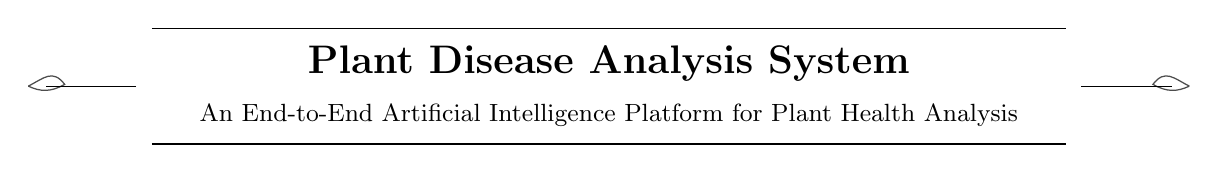
\begin{tikzpicture}
  \node[inner xsep=0.45cm,inner ysep=0.22cm,align=center] (title) {%
    {\Large\bfseries Plant Disease Analysis System}\\[0.18cm]
    {\small An End-to-End Artificial Intelligence Platform for Plant Health Analysis}
  };
  \draw[line width=0.45pt] ([xshift=-0.15cm]title.north west) -- ([xshift=0.15cm]title.north east);
  \draw[line width=0.45pt] ([xshift=-0.15cm]title.south west) -- ([xshift=0.15cm]title.south east);
  \draw[line width=0.35pt] ([xshift=-0.35cm]title.west) -- ++(-1.15cm,0);
  \draw[line width=0.35pt] ([xshift=0.35cm]title.east) -- ++(1.15cm,0);
  \begin{scope}[shift={([xshift=-1.72cm]title.west)},scale=0.28,opacity=0.7]
    \draw[line width=0.45pt] (0,0) .. controls (0.7,0.35) and (1.1,0.8) .. (1.65,0.08)
      .. controls (1.02,-0.28) and (0.55,-0.26) .. (0,0);
  \end{scope}
  \begin{scope}[shift={([xshift=1.72cm]title.east)},xscale=-0.28,yscale=0.28,opacity=0.7]
    \draw[line width=0.45pt] (0,0) .. controls (0.7,0.35) and (1.1,0.8) .. (1.65,0.08)
      .. controls (1.02,-0.28) and (0.55,-0.26) .. (0,0);
  \end{scope}
\end{tikzpicture}\\[0.72cm]

{\normalsize\bfseries TEAM MEMBERS}\\[0.25cm]
\begin{tabular}{@{}l@{\hspace{1.1cm}}r@{}}
Armia Gamal Fakry & 352250706 \\
Sherif Karam Zaki & 352250808 \\
Sara Essam Ibrahim & 352250785 \\
Ziad Walid Mokhtar & 352250783 \\
Shada Ayman Eldin Ahmed & 352250804 \\
Peter Bolbol Sefin & 352250738 \\
Salsabel Esmail Hussin & 352250787 \\
\end{tabular}

\vspace{0.75cm}

{\large\bfseries SUPERVISED BY}\\[0.35cm]

{\Large\bfseries Dr. Mourad Raafat}\\[0.18cm]

{\normalsize Professor of Mathematical Statistics}

\vfill
\end{titlepage}

\cleardoublepage
%==============================================================================
% DEDICATION
%==============================================================================

\thispagestyle{plain}
\addcontentsline{toc}{chapter}{Dedication}
\markboth{Dedication}{Dedication}

\vfill

\begin{center}
\begin{minipage}{0.78\textwidth}
\centering
{\Large\itshape

To the farmers around the world,\\[0.45cm]

whose dedication, resilience, and unwavering commitment\\
to feeding communities continue to inspire innovation\\
and remind us of the vital role agriculture plays\\
in sustaining life and shaping the future.\\[1.2cm]

To our families,\\[0.45cm]

for their endless love, encouragement, patience,\\
and unwavering belief in us throughout this journey.\\
Their support gave us the strength\\
to overcome every challenge and pursue excellence.\\[1.2cm]

Finally,\\[0.45cm]

to everyone who believes that artificial intelligence\\
can contribute to a more sustainable\\
and resilient agricultural future.

}
\end{minipage}
\end{center}

\vfill
\cleardoublepage
%==============================================================================
% ACKNOWLEDGEMENT
%==============================================================================

\chapter*{Acknowledgements}
\addcontentsline{toc}{chapter}{Acknowledgements}
\markboth{Acknowledgements}{Acknowledgements}

The authors gratefully acknowledge the guidance and unwavering support of \textbf{Dr.\ Mourad Raafat}, whose expert supervision, constructive criticism, and continuous encouragement were instrumental throughout every phase of this project's development. His deep knowledge of artificial intelligence and software engineering fundamentally shaped the quality of this work.

The team extends sincere appreciation to the \textbf{Department of Computer Science and Statistics} at the \textbf{Faculty of Science, Helwan University}, for providing an intellectually stimulating academic environment and the computational resources necessary to conduct the extensive model training experiments described herein.

Gratitude is likewise extended to the open-source communities and academic researchers behind the datasets, frameworks, and tools that form the technical foundation of \nabta, including the contributors to PlantVillage, PlantDoc, the Ultralytics \yolo ecosystem, and the underlying deep learning frameworks employed during model development. Without their freely shared contributions, projects of this nature would not be possible.

Finally, the authors dedicate sincere thanks to their families for their patience, moral support, and encouragement throughout the duration of this project.

\cleardoublepage
%==============================================================================
% ABSTRACT
%==============================================================================

\chapter*{Abstract}
\addcontentsline{toc}{chapter}{Abstract}
\markboth{Abstract}{Abstract}

\noindent
This project presents \nabta, a comprehensive AI-powered smart agriculture platform that integrates computer vision, machine learning, explainable artificial intelligence, and large language models to support intelligent agricultural decision-making. The platform provides an end-to-end ecosystem for automated plant disease diagnosis, crop recommendation, irrigation recommendation, and AI-assisted agricultural consultation through a unified web-based application. By combining multiple artificial intelligence technologies within a single production-ready platform, \nabta aims to improve agricultural productivity, optimize resource utilization, and promote sustainable farming practices.

The plant disease analysis module employs a multi-stage computer vision pipeline. \gls{yolov8} performs real-time object detection to localize infected leaf regions, followed by a \unet segmentation model with an EfficientNet-B0 encoder that isolates leaf tissue from complex backgrounds using pixel-level segmentation. The refined leaf images are then classified by a custom \gls{cnn} trained on a unified dataset containing more than \textbf{120,000} images across \textbf{102} healthy and diseased plant classes. To improve model transparency and user trust, \gls{gradcam} is incorporated to generate visual explanations highlighting the image regions responsible for each prediction.

Beyond disease diagnosis, \nabta integrates intelligent decision-support services for precision agriculture. A Random Forest-based crop recommendation model analyzes soil properties, including Nitrogen (N), Phosphorus (P), Potassium (K), soil type, weather conditions, and environmental factors to recommend the most suitable crops for cultivation. In addition, the platform includes two irrigation intelligence modules: a Random Forest classification model for irrigation decision-making and a Random Forest regression model for estimating crop water requirements, enabling efficient irrigation planning and optimized water resource management.

To further enhance user interaction, the platform incorporates a domain-specific conversational assistant powered by the Cohere \gls{api} and Retrieval-Augmented Generation (\gls{rag}). The assistant provides evidence-based disease treatment recommendations, crop management guidance, irrigation advice, and general agricultural consultations in both Arabic and English. All intelligent services are deployed through a high-performance asynchronous \fastapi backend and presented via a responsive React.js dashboard featuring image analysis, recommendation modules, historical records, analytics, authentication, and user management.

Experimental evaluation demonstrates the effectiveness of the proposed AI modules. The plant disease classification model achieved an overall accuracy of \textbf{95.0\%} across \textbf{102} healthy and diseased plant classes trained on more than \textbf{120,000} images. The YOLOv8x detection model achieved a validation Precision of \textbf{72.9\%}, Recall of \textbf{72.6\%}, and an \gls{map}@0.50 of \textbf{78.8\%}, while the proposed U-Net segmentation model achieved a best mean \gls{iou} of \textbf{94.73\%}. The crop recommendation model achieved a test accuracy of \textbf{85.13\%} with a cross-validation accuracy of \textbf{84.8\%}, while the irrigation decision model achieved a test accuracy of \textbf{98.53\%}. Furthermore, the irrigation water requirement regression model achieved a test coefficient of determination (\(R^2\)) of \textbf{95.22\%} with a mean absolute error of only \textbf{13.47 mm}. Collectively, these results demonstrate the capability of \nabta to deliver accurate plant disease diagnosis, intelligent agricultural recommendations, efficient irrigation management, and scalable AI-powered decision support for modern precision agriculture.

\vspace{1em}
\noindent\textbf{Keywords:} Smart agriculture, plant disease detection, crop recommendation, irrigation recommendation, deep learning, machine learning, Random Forest, YOLOv8, U-Net, convolutional neural networks, Grad-CAM, explainable AI, retrieval-augmented generation, FastAPI, precision agriculture.

\cleardoublepage
% Generated navigation pages for the report.

\pagestyle{fancy}
{
  \hypersetup{hidelinks}
  \tableofcontents
  \cleardoublepage
  \listoffigures
  \cleardoublepage
  \listoftables
  \cleardoublepage
}

\glsaddall
\printnoidxglossary[type=\acronymtype,title={List of Abbreviations},toctitle={List of Abbreviations}]
\cleardoublepage


\mainmatter
\pagestyle{fancy}

%==============================================================================
% CHAPTER 1 --- INTRODUCTION
%==============================================================================

\chapter{Introduction}
\label{chap:introduction}

\chapterquote{Agriculture is our wisest pursuit, because it will in the end contribute most to real wealth, good morals, and happiness.}{Thomas Jefferson}

\section{Background and Context}
\label{sec:intro_background}

Agriculture constitutes one of the most fundamental pillars of human civilisation, providing sustenance, economic activity, and employment to billions of people across all continents. Despite dramatic advances in industrial food production and globalised supply chains, the security of the world's crop yields remains perpetually vulnerable to biological threats. Among these threats, plant pathogens---encompassing fungal infections, bacterial blights, viral diseases, and parasitic infestations---represent perhaps the most persistent and damaging challenge facing agricultural communities worldwide.

The \gls{fao} estimates that plant diseases are collectively responsible for the destruction of up to \textbf{40\%} of all food crops globally on an annual basis~\cite{fao2021}. This staggering figure translates not merely to economic losses measured in billions of dollars, but to food insecurity for vulnerable populations, reduced livelihoods for smallholder farmers, and the unnecessary over-application of chemical pesticides that degrades soil health and contaminates water systems. The problem is particularly acute in developing nations, where limited access to agronomic expertise and diagnostic infrastructure renders early intervention exceptionally difficult.

Historically, the identification and management of plant diseases has depended heavily on the manual inspection capabilities of trained agronomists and plant pathologists. Such experts evaluate macroscopic and microscopic symptoms---discolouration patterns, lesion morphology, necrotic tissue boundaries, and spore structures---to arrive at a differential diagnosis. This approach, while clinically valid, suffers from three fundamental operational limitations: it is \textit{time-intensive}, requiring sustained expert availability; it is \textit{geographically constrained}, given the scarcity of credentialled specialists in many agricultural regions; and it is inherently \textit{non-scalable}, since even an experienced agronomist can examine only a limited number of field samples within a practical timeframe.

The convergence of deep learning, computer vision, and cloud computing over the past decade has opened genuinely transformative possibilities for automated, scalable, and accessible plant disease diagnosis. Landmark work such as that of Mohanty~et~al.~\cite{mohanty2016} demonstrated that convolutional neural networks trained on curated leaf-image datasets could achieve accuracy levels competitive with---and in some cases exceeding---those of human experts under controlled photographic conditions. Subsequent advances in object detection architectures, notably the YOLO family~\cite{jocher2023yolov8}, and in semantic segmentation networks, most prominently the U-Net architecture~\cite{ronneberger2015}, have further expanded the toolkit available for intelligent agricultural analysis. Alongside these discriminative models, the emergence of large language models and retrieval-augmented generation~\cite{lewis2020rag} has created new possibilities for deploying expert knowledge at scale through conversational interfaces.

\section{Problem Statement}
\label{sec:intro_problem}

Despite the technological advances described above, a substantial gap persists between isolated academic demonstrations and practical, deployed systems that farmers and agricultural workers can readily access and trust. Several specific, interconnected challenges characterise this gap and motivated the development of the \nabta system:

\begin{enumerate}[leftmargin=*, label=\textbf{P\arabic*.}]
  \item \textbf{Stage-Specific Vulnerability:} Plant pathogens typically exhibit their most characteristic visual symptoms only in intermediate or advanced disease stages. Early-stage infections, when intervention would be most cost-effective, present subtle lesion patterns that are easily overlooked by non-specialist observers or overwhelmed by the complex visual noise present in field photographs---soil backgrounds, uneven lighting, overlapping foliage, and shadow gradients.

  \item \textbf{Expert Scarcity and Geographic Inaccessibility:} Qualified plant pathologists and agronomists are unevenly distributed across agricultural geographies. Rural and remote farming communities in developing nations face the most acute shortfall, with access to specialist consultations requiring either costly field visits or lengthy delays.

  \item \textbf{Financial Constraints of Manual Diagnosis:} Continuous reliance on human expert evaluation is economically unsustainable for smallholder farmers operating on tight margins. Laboratory analysis, travel costs, and specialist fees collectively impose a recurring financial burden that suppresses diagnostic uptake.

  \item \textbf{Epidemic Spreading and Delayed Response:} Without rapid, on-demand diagnostic capabilities, infected plants may go undetected for extended periods. During this interval, pathogen spores and vectors spread to neighbouring plants and adjacent fields, escalating localised infections into wide-scale epidemic events before any containment response is mounted.

  \item \textbf{Misdiagnosis Risk and Pesticide Misuse:} Incorrect identification of a pathogen, whether by an under-qualified observer or by a single-stage, context-insensitive AI model, leads directly to the application of inappropriate chemical treatments. Such misuse wastes agricultural inputs, accelerates the development of chemical resistance among pathogen populations, and introduces unnecessary environmental contamination.

  \item \textbf{Scalability Ceiling of Human-Dependent Systems:} Traditional diagnostic workflows cannot be linearly scaled to monitor extensive agricultural operations. Large farms with hundreds of hectares under cultivation require a form of continuous, automated surveillance that no human workforce can economically provide.
\end{enumerate}

\section{Motivation}
\label{sec:intro_motivation}

The motivation for developing \nabta arises from the recognition that the individual technologies required to address the above problems already exist in mature or near-mature forms within the research literature. What is absent is a coherent, production-quality system that combines these technologies in a principled architectural framework, exposes them through an accessible user interface suitable for non-technical agricultural workers, and deploys them with the security, reliability, and performance characteristics demanded by real-world operational environments.

Furthermore, the authors were motivated by the observation that existing plant disease classification systems overwhelmingly adopt single-stage pipelines---one model receives a raw field image and produces a class label. This design choice, while computationally economical, fundamentally ignores the compound degradation in model confidence caused by complex photographic backgrounds. A hierarchical pipeline that progressively refines the input---first isolating the leaf region, then segmenting its tissue boundaries, and finally classifying the isolated pathological features---constitutes a significantly more robust approach to real-world conditions.

\section{Project Objectives}
\label{sec:intro_objectives}

The \nabta project pursues the following primary engineering and research objectives:

\begin{enumerate}[leftmargin=*, label=\textbf{O\arabic*.}]
  \item \textbf{Unified Multi-Model AI Pipeline:} Design and implement a sequential, multi-stage computer vision pipeline that combines object detection (\yolo), semantic segmentation (\unet), and image classification (\cnn) into a cohesive inference workflow acting on a single raw input image.

  \item \textbf{High-Accuracy Pathogen Classification:} Achieve classification accuracy exceeding 95\% across a dataset spanning 102 distinct disease categories and healthy plant states, encompassing a diverse range of crop species and pathogen types.

  \item \textbf{Explainable AI Integration:} Incorporate \gradcam visualisations into the inference output to ensure that model decisions are interpretable and verifiable by agronomists and non-technical users alike, thereby building operational trust in the system.

  \item \textbf{Intelligent Consultation Layer:} Develop a domain-restricted, multilingual conversational AI module using \gls{rag} and the Cohere \gls{llm} platform, capable of delivering expert-quality treatment prescriptions grounded in curated agricultural knowledge.

  \item \textbf{Production-Ready Cloud Deployment:} Architect a high-performance asynchronous backend using \fastapi, capable of servicing concurrent field requests with sub-second inference latency.

  \item \textbf{Accessible, Responsive Interface:} Deliver a fully featured, mobile-responsive web application in React.js that enables farmers with minimal technical literacy to submit plant images and receive comprehensive diagnostic reports.

  \item \textbf{Robust Security Architecture:} Implement a multi-layered security posture encompassing Firebase Authentication, HTTPS encryption, and secure API key management.
\end{enumerate}

\section{Project Scope}
\label{sec:intro_scope}

The scope of the \nabta project encompasses the full software development lifecycle of the described system, from requirements analysis and architectural design through model training, system integration, and deployment. The project operates within the following defined boundaries:

The classification capability is bounded by the training data: the system diagnoses plant diseases within the 102 classes represented in the combined training corpus, which includes crops such as tomato, potato, pepper, apple, grape, corn, rice, cotton, mango, eggplant, strawberry, orange, and cucumber, among others. Extension to additional species and pathogen types is identified as a future research direction.

The system is designed for \textit{leaf-level image analysis}. Diagnosis derived from full-plant or field-view imagery without sufficient leaf prominence is not the primary design target, although the \yolo detection stage partially compensates for this by isolating leaf-level regions of interest even within complex scene compositions.

The chatbot consultation interface is intentionally domain-restricted. The system rejects queries outside the agricultural domain to maintain response reliability and prevent the dissemination of hallucinated advice for off-topic subjects.

\section{Contributions}
\label{sec:intro_contributions}

The principal technical contributions of the \nabta project are summarised as follows:

\begin{itemize}[leftmargin=*]
  \item \textbf{End-to-End Multi-Stage Pipeline:} A novel sequential pipeline architecture combining \yolo detection, \unet segmentation, and \cnn classification, demonstrated to achieve superior robustness over single-stage baselines on field-condition imagery.

  \item \textbf{Large-Scale Training Corpus:} The curation and integration of a combined training dataset exceeding 120,000 images across 102 classes, sourced from seven distinct open-source agricultural repositories, with systematic balancing and augmentation.

  \item \textbf{Integrated \gradcam Explainability:} The first demonstration, to the authors' knowledge, of real-time \gradcam overlay delivery within a production web application targeting agricultural end-users.

  \item \textbf{\rag-Augmented Agricultural Chatbot:} A deployable, domain-restricted conversational AI module providing treatment recommendations grounded in a curated vector knowledge base, evaluated and validated by agricultural domain experts.

  \item \textbf{Production Deployment Architecture:} A complete, documented system architecture combining \fastapi, Firebase, a vector database, and React.js, designed for immediate deployability in cloud environments.
\end{itemize}

\section{Document Organisation}
\label{sec:intro_organisation}

The remainder of this document is structured as follows. \chapref{chap:literature_review} presents the domain background, related work, requirements analysis, and user-facing use cases. \chapref{chap:methodology} details the data collection strategy, preprocessing protocols, training corpus composition, and model development methodology. \chapref{chap:design} describes the full system architecture, backend design, frontend design, database schema, API specification, and modelling artefact placeholders. \chapref{chap:implementation} documents the technologies employed, the development environment, and key implementation details with illustrative screenshot placeholders. \chapref{chap:results} presents evaluation metrics, testing evidence, and comparative discussion. Finally, \chapref{chap:conclusion} synthesises the project's achievements, acknowledges its limitations, and outlines the roadmap for future enhancement.

%==============================================================================
% CHAPTER 2 -- LITERATURE REVIEW AND SYSTEM ANALYSIS
%==============================================================================

\chapter{Literature Review and System Analysis}
\label{chap:literature_review}

\chapterquote{Good software, like good writing, requires understanding the audience before writing the first line.}{Anonymous}

\section{Related Work}
\label{sec:related_work}

Plant disease diagnosis has evolved from manual visual inspection toward computer vision systems that can classify disease symptoms from leaf images. Early deep learning studies, including Mohanty et al.~\cite{mohanty2016}, demonstrated the feasibility of convolutional neural networks on controlled datasets such as PlantVillage. Later work introduced stronger backbones, object detection models, segmentation networks, and explainability techniques to improve robustness under field conditions.

The \nabta project builds on this body of work by combining object detection, segmentation, classification, and retrieval-augmented consultation in one deployable workflow. Unlike single-stage classifiers that process the whole image directly, the proposed pipeline progressively isolates the leaf region, removes background noise, classifies the disease, and explains the decision through \gradcam.

\section{Overview}
\label{sec:analysis_overview}

System analysis constitutes the foundational phase in which the problem domain is formally examined and translated into a structured set of requirements that guide all subsequent design and implementation activities. This chapter presents a comprehensive requirements analysis for the \nabta system, encompassing both functional and non-functional specifications, a characterisation of the system's stakeholder groups and user roles, and a structured inventory of use cases and test scenarios.

The analysis was conducted through a combination of literature review, user-centric need identification, and iterative refinement by the development team in consultation with the project supervisor. The resulting requirements document served as the primary contract specification governing system development.

\section{Stakeholder Analysis}
\label{sec:analysis_stakeholders}

The \nabta system serves a heterogeneous community of stakeholders with distinct interests and interaction modalities:

\begin{table}[H]
  \centering
  \caption{Stakeholder Groups and Their Primary Interests}
  \label{tab:stakeholders}
  \renewcommand{\arraystretch}{1.4}
  \begin{tabularx}{\textwidth}{>{\bfseries}l X X}
    \toprule
    Stakeholder & Role & Primary Interest \\
    \midrule
    Field Farmers & Primary end-users & Rapid, reliable disease identification for crop protection \\
    Agronomists & Domain experts and validators & Verifiable, evidence-based diagnostic output \\
    Agricultural Researchers & Secondary users & Access to aggregated disease distribution data \\
    System Administrators & Technical operators & System uptime, security, and performance monitoring \\
    Project Supervisors & Academic oversight & Research quality and documentation standards \\
    Helwan University & Institutional sponsor & Demonstrable academic and practical contribution \\
    \bottomrule
  \end{tabularx}
\end{table}

\section{User Roles}
\label{sec:analysis_roles}

The system defines three distinct user roles with differentiated access privileges:

\subsection{Free-Tier User}
\label{subsec:free_user}
The free-tier user represents the baseline access level, available to all registered accounts at no cost. Free-tier users may upload plant images for sequential pipeline analysis, view the resulting detection bounding boxes, segmentation masks, classification labels, confidence scores, and \gradcam heatmaps. Access to the AI chatbot consultation interface is provided with daily usage limitations. Historical analysis records are retained for a defined rolling window period.

\subsection{Pro-Tier User}
\label{subsec:pro_user}
Pro-tier users ($\$20$/month) access the full feature set without usage restrictions. Additional capabilities exclusive to pro-tier accounts include unrestricted daily analysis submissions, the ability to upload custom datasets for personalised model fine-tuning, access to the comprehensive Nabta Smart Analysis Center dashboard with detailed farm-level infection timeline visualisations, and the export of analytical reports in PDF format.

\subsection{System Administrator}
\label{subsec:admin_user}
System administrators possess elevated privileges for user management, system health monitoring, model version management, and content moderation within the knowledge base used by the RAG consultation module.

\section{Functional Requirements}
\label{sec:functional_requirements}

Functional requirements specify the behavioural capabilities that the \nabta system must provide. Each requirement is assigned a unique identifier for traceability.

\subsection{Authentication and Account Management}
\label{subsec:fr_auth}

\begin{table}[H]
  \centering
  \caption{Functional Requirements: Authentication and Account Management}
  \label{tab:fr_auth}
  \renewcommand{\arraystretch}{1.4}
  \begin{tabularx}{\textwidth}{l l X}
    \toprule
    \textbf{ID} & \textbf{Priority} & \textbf{Requirement Description} \\
    \midrule
    FR-01 & High & The system shall allow new users to register accounts via an email and password mechanism facilitated by Firebase Authentication. \\
    FR-02 & High & The system shall authenticate registered users via secure login and maintain authenticated session state. \\
    FR-03 & High & The system shall provide a password reset workflow via a registered email address. \\
    FR-04 & Medium & The system shall send a welcome email to newly registered users upon successful account creation. \\
    FR-05 & Medium & The system shall maintain differentiated access controls between free-tier and pro-tier user accounts. \\
    \bottomrule
  \end{tabularx}
\end{table}

\subsection{Plant Image Analysis}
\label{subsec:fr_analysis}

\begin{table}[H]
  \centering
  \caption{Functional Requirements: Plant Image Analysis}
  \label{tab:fr_analysis}
  \renewcommand{\arraystretch}{1.4}
  \begin{tabularx}{\textwidth}{l l X}
    \toprule
    \textbf{ID} & \textbf{Priority} & \textbf{Requirement Description} \\
    \midrule
    FR-06 & High & The system shall accept plant leaf images in JPEG and PNG formats up to a maximum file size of 5 MB. \\
    FR-07 & High & The system shall perform object detection on uploaded images using the YOLOv8 model to identify and bound infected leaf regions. \\
    FR-08 & High & The system shall perform semantic segmentation on extracted ROI crops using the U-Net model with EfficientNet-B0 encoder. \\
    FR-09 & High & The system shall classify the segmented and refined leaf image into one of 102 target disease/healthy classes using the custom CNN. \\
    FR-10 & High & The system shall generate Grad-CAM gradient heatmaps overlaid on the classification input image. \\
    FR-11 & High & The system shall return the plant name, disease name, confidence score, infection severity percentage, and Grad-CAM overlay image to the client. \\
    FR-12 & High & The system shall store all analysis results associated with the authenticated user's account. \\
    FR-13 & Medium & The system shall generate and allow download of a PDF report summarising the diagnosis. \\
    \bottomrule
  \end{tabularx}
\end{table}

\subsection{AI Consultation Chatbot}
\label{subsec:fr_chatbot}

\begin{table}[H]
  \centering
  \caption{Functional Requirements: AI Consultation Chatbot}
  \label{tab:fr_chatbot}
  \renewcommand{\arraystretch}{1.4}
  \begin{tabularx}{\textwidth}{l l X}
    \toprule
    \textbf{ID} & \textbf{Priority} & \textbf{Requirement Description} \\
    \midrule
    FR-14 & High & The system shall provide a conversational AI interface for agricultural queries powered by the Cohere LLM and RAG pipeline. \\
    FR-15 & High & The system shall restrict chatbot responses to agricultural domain queries, rejecting off-topic prompts with a polite refusal message. \\
    FR-16 & High & The system shall support both Arabic and English input and response languages. \\
    FR-17 & High & The chatbot shall provide structured responses covering overview, cause, infection analysis, severity status, organic treatment, chemical treatment, prevention guidelines, and warning signs. \\
    FR-18 & Medium & The chatbot shall generate a final health score and priority action list at the conclusion of each consultation session. \\
    \bottomrule
  \end{tabularx}
\end{table}

\subsection{Analytics Dashboard}
\label{subsec:fr_dashboard}

\begin{table}[H]
  \centering
  \caption{Functional Requirements: Analytics Dashboard}
  \label{tab:fr_dashboard}
  \renewcommand{\arraystretch}{1.4}
  \begin{tabularx}{\textwidth}{l l X}
    \toprule
    \textbf{ID} & \textbf{Priority} & \textbf{Requirement Description} \\
    \midrule
    FR-19 & High & The system shall display a disease distribution chart summarising historical analysis counts by disease type. \\
    FR-20 & High & The system shall display an infection timeline chart enabling users to observe seasonal and temporal infection trends. \\
    FR-21 & Medium & The system shall display a ranking of the most frequently analysed plant species. \\
    FR-22 & Medium & The system shall maintain and display a paginated log of recent analyses with timestamps, species, and disease tags. \\
    FR-23 & Low & Pro-tier users shall be able to export dashboard data in standard tabular formats. \\
    \bottomrule
  \end{tabularx}
\end{table}

\section{Non-Functional Requirements}
\label{sec:nonfunctional_requirements}

\begin{table}[H]
  \centering
  \caption{Non-Functional Requirements}
  \label{tab:nfr}
  \renewcommand{\arraystretch}{1.5}
  \begin{tabularx}{\textwidth}{l l X}
    \toprule
    \textbf{ID} & \textbf{Category} & \textbf{Requirement} \\
    \midrule
    NFR-01 & Performance   & The end-to-end inference pipeline shall complete within 0.4 seconds for standard resolution inputs under nominal server load. \\
    NFR-02 & Scalability   & The backend shall support concurrent multi-user inference requests through asynchronous processing. \\
    NFR-03 & Accuracy      & The CNN classifier shall achieve a minimum accuracy of 95\% on the held-out validation set at release. \\
    NFR-04 & Reliability   & The system shall maintain an uptime target of at least 99.5\% during active deployment. \\
    NFR-05 & Security      & All client-server communication shall be encrypted via HTTPS. User authentication shall be managed through Firebase, and API keys shall be stored securely using environment variable vaults. \\
    NFR-06 & Usability     & The web interface shall be fully functional on modern desktop and mobile browsers with no additional plugin installation required. \\
    NFR-07 & Maintainability & System components shall be modularly decoupled such that individual model nodes can be upgraded independently without requiring refactoring of frontend or unrelated backend modules. \\
    NFR-08 & Accessibility & The interface shall support bilingual (Arabic and English) content rendering. \\
    NFR-09 & Portability   & The backend shall be containerisable via Docker for cloud-agnostic deployment. \\
    \bottomrule
  \end{tabularx}
\end{table}

\section{Use Cases}
\label{sec:use_cases}

\subsection{UC-01: User Registration}
\label{subsec:uc01}

\begin{table}[H]
  \centering
  \caption{Use Case: User Registration}
  \label{tab:uc01}
  \renewcommand{\arraystretch}{1.4}
  \begin{tabularx}{\textwidth}{l X}
    \toprule
    \textbf{Field}           & \textbf{Details} \\
    \midrule
    Use Case ID              & UC-01 \\
    Name                     & User Registration \\
    Actor(s)                 & New User \\
    Preconditions            & User has not previously registered an account \\
    Main Success Scenario    & User submits registration form $\rightarrow$ Firebase Auth validates credentials $\rightarrow$ Account created $\rightarrow$ Welcome email dispatched \\
    Alternative Scenario     & Email already in use $\rightarrow$ System displays error; user prompted to log in or reset password \\
    Postconditions           & Authenticated user session established; user redirected to dashboard \\
    \bottomrule
  \end{tabularx}
\end{table}

\subsection{UC-02: Plant Image Upload and Analysis}
\label{subsec:uc02}

\begin{table}[H]
  \centering
  \caption{Use Case: Plant Image Upload and Analysis}
  \label{tab:uc02}
  \renewcommand{\arraystretch}{1.4}
  \begin{tabularx}{\textwidth}{l X}
    \toprule
    \textbf{Field}           & \textbf{Details} \\
    \midrule
    Use Case ID              & UC-02 \\
    Name                     & Plant Image Upload and Analysis \\
    Actor(s)                 & Authenticated User (Free or Pro Tier) \\
    Preconditions            & User is logged in; image file meets format and size requirements \\
    Main Success Scenario    & User uploads image $\rightarrow$ Backend preprocesses image $\rightarrow$ YOLOv8 detects ROI $\rightarrow$ U-Net segments leaf $\rightarrow$ CNN classifies disease $\rightarrow$ Grad-CAM generated $\rightarrow$ Results returned to frontend $\rightarrow$ Results stored in database \\
    Alternative Scenario A   & No leaf detected by YOLO $\rightarrow$ System returns informative error advising improved image quality \\
    Alternative Scenario B   & File exceeds 5MB limit $\rightarrow$ Upload rejected with size-limit notification \\
    Postconditions           & Analysis result persisted; user viewing diagnosis report \\
    \bottomrule
  \end{tabularx}
\end{table}

\subsection{UC-03: AI Chatbot Consultation}
\label{subsec:uc03}

\begin{table}[H]
  \centering
  \caption{Use Case: AI Chatbot Consultation}
  \label{tab:uc03}
  \renewcommand{\arraystretch}{1.4}
  \begin{tabularx}{\textwidth}{l X}
    \toprule
    \textbf{Field}           & \textbf{Details} \\
    \midrule
    Use Case ID              & UC-03 \\
    Name                     & AI Chatbot Consultation \\
    Actor(s)                 & Authenticated User \\
    Preconditions            & User is logged in; daily query limit not exceeded \\
    Main Success Scenario    & User submits agricultural query $\rightarrow$ Query processed by RAG pipeline $\rightarrow$ Relevant documents retrieved from vector DB $\rightarrow$ Cohere LLM generates structured response $\rightarrow$ Response rendered in chat panel \\
    Alternative Scenario     & Non-agricultural query submitted $\rightarrow$ Domain restriction filter activates; polite refusal returned \\
    Postconditions           & Response displayed; conversation history maintained in session \\
    \bottomrule
  \end{tabularx}
\end{table}

\subsection{UC-04: PDF Report Generation}
\label{subsec:uc04}

\begin{table}[H]
  \centering
  \caption{Use Case: PDF Report Generation}
  \label{tab:uc04}
  \renewcommand{\arraystretch}{1.4}
  \begin{tabularx}{\textwidth}{l X}
    \toprule
    \textbf{Field}           & \textbf{Details} \\
    \midrule
    Use Case ID              & UC-04 \\
    Name                     & PDF Report Generation \\
    Actor(s)                 & Authenticated User \\
    Preconditions            & At least one analysis result exists for the user \\
    Main Success Scenario    & User requests PDF report $\rightarrow$ Backend compiles diagnosis, images, and treatment information $\rightarrow$ PDF generated and returned as download \\
    Postconditions           & PDF file downloaded to user's device \\
    \bottomrule
  \end{tabularx}
\end{table}

\subsection{UC-05: Subscription Upgrade}
\label{subsec:uc05}

\begin{table}[H]
  \centering
  \caption{Use Case: Subscription Upgrade}
  \label{tab:uc05}
  \renewcommand{\arraystretch}{1.4}
  \begin{tabularx}{\textwidth}{l X}
    \toprule
    \textbf{Field}           & \textbf{Details} \\
    \midrule
    Use Case ID              & UC-05 \\
    Name                     & Pro-Tier Subscription Upgrade \\
    Actor(s)                 & Free-Tier User \\
    Preconditions            & User is logged in with a free-tier account \\
    Main Success Scenario    & User navigates to upgrade page $\rightarrow$ Payment processed $\rightarrow$ Account tier updated in Firebase $\rightarrow$ Pro features unlocked \\
    Extended Feature         & Unlocks custom dataset upload for personalised model training \\
    Postconditions           & User account upgraded; pro-tier dashboard features accessible \\
    \bottomrule
  \end{tabularx}
\end{table}

\section{Test Cases}
\label{sec:test_cases}

\begin{table}[H]
  \centering
  \caption{System Test Case Inventory (Part 1 of 2)}
  \label{tab:test_cases}
  \small
  \setlength{\tabcolsep}{4pt}
  \begin{tabularx}{\textwidth}{@{}L{1.25cm} L{1.45cm} Y Y@{}}
    \toprule
    \textbf{TC ID} & \textbf{Linked UC} & \textbf{Test Description} & \textbf{Expected Outcome} \\
    \midrule
    \textbf{TC-01} & UC-01 & Submit registration with a valid email and strong password & Account created; welcome email received \\
    \textbf{TC-02} & UC-01 & Submit registration with an existing email & Error displayed; no duplicate account created \\
    \textbf{TC-03} & UC-02 & Upload a clear tomato leaf image with visible blight lesions & Early blight classified with $\geq 90\%$ confidence \\
    \textbf{TC-04} & UC-02 & Upload an image exceeding 5 MB & Upload rejected with an appropriate message \\
    \textbf{TC-05} & UC-02 & Upload an image without visible leaf content & No ROI returned; user prompted to retry \\
    \textbf{TC-06} & UC-02 & Upload a healthy leaf image & Healthy class label returned \\
    \textbf{TC-07} & UC-02 & Verify that the Grad-CAM overlay accompanies the result & Heatmap returned and rendered by the frontend \\
    \bottomrule
  \end{tabularx}
\end{table}

\begin{table}[H]
  \centering
  \caption{System Test Case Inventory (Part 2 of 2)}
  \small
  \setlength{\tabcolsep}{4pt}
  \begin{tabularx}{\textwidth}{@{}L{1.25cm} L{1.45cm} Y Y@{}}
    \toprule
    \textbf{TC ID} & \textbf{Linked UC} & \textbf{Test Description} & \textbf{Expected Outcome} \\
    \midrule
    \textbf{TC-08} & UC-03 & Ask about treatment for a tomato fungal disease & Organic and chemical treatment sections returned \\
    \textbf{TC-09} & UC-03 & Submit a non-agricultural query & Polite domain-restriction response returned \\
    \textbf{TC-10} & UC-03 & Submit a query in Arabic & Response returned in Arabic \\
    \textbf{TC-11} & UC-04 & Request a PDF report after an analysis & Report downloaded with the diagnosis summary \\
    \textbf{TC-12} & UC-05 & Upgrade a free account through the payment flow & Pro features enabled; usage limits updated \\
    \textbf{TC-13} & NFR-01 & Measure total pipeline latency for a standard image & Response time $\leq 400$ ms \\
    \textbf{TC-14} & NFR-05 & Inspect network traffic during authentication & HTTPS used; no plaintext credentials observed \\
    \bottomrule
  \end{tabularx}
\end{table}

%==============================================================================
% CHAPTER 4 --- METHODOLOGY
%==============================================================================

\chapter{Methodology}
\label{chap:methodology}

\chapterquote{In God we trust. All others must bring data.}{W. Edwards Deming}

\section{Overview}
\label{sec:meth_overview}

The methodological framework underlying the \nabta system reflects a principled, iterative approach to the development and validation of machine learning models for agricultural pathogen diagnosis. This chapter details each stage of the data science lifecycle as applied to the project: dataset collection and curation, preprocessing and augmentation strategies, the architecture and training of each component model, and the validation strategy employed to evaluate generalisation performance. The design decisions described herein were guided by a core objective of maximising real-world robustness rather than benchmark-optimised performance on curated laboratory data.

\section{Data Collection}
\label{sec:data_collection}

\subsection{Dataset Strategy}
\label{subsec:dataset_strategy}

The fundamental challenge in building a robust plant disease classifier is not merely the acquisition of data, but the acquisition of sufficiently diverse data that represents the heterogeneity of real field conditions. A single-source dataset, however large, tends to encode the photographic style, lighting conditions, and crop species distribution of its contributing institution. To mitigate this domain-bias problem, the \nabta training corpus was assembled by integrating seven distinct publicly available agricultural image repositories.

The combined dataset totals in excess of \textbf{120,000 annotated images} spanning \textbf{102 target classes}---comprising disease states across multiple crop species as well as corresponding healthy class labels for each species. This multi-source fusion constitutes a substantially more challenging and representative training distribution than any single component dataset.

\subsection{Component Datasets}
\label{subsec:datasets}

\begin{table}[H]
  \centering
  \caption{Training Dataset Components for the NABTA Classification Model}
  \label{tab:datasets}
  \small
  \renewcommand{\arraystretch}{1.35}
  \setlength{\tabcolsep}{4pt}
  \begin{tabularx}{\textwidth}{L{2.7cm} Y L{2.5cm} L{2.4cm}}
    \toprule
    \textbf{Dataset} & \textbf{Description} & \textbf{Focus} & \textbf{Source} \\
    \midrule
    PlantVillage & Benchmark dataset of 54,305 images across 14 crops and 26 diseases; laboratory-controlled conditions & Classification & Kaggle / Penn State \\
    PlantDoc & 2,569 images collected under diverse outdoor conditions; includes 13 plant species and 17 disease classes & Detection \& Classification & Open Source \\
    Plant Diseases Training Dataset & Supplementary multi-crop collection for generalisation improvement & Classification & Kaggle \\
    Bangladesh Crop Dataset & Region-specific rice and jute crop images for geographic diversity & Classification & Kaggle \\
    Rice Leaf Disease Dataset & Dedicated collection for bacterial blight, blast, and tungro diseases in rice & Classification & Kaggle \\
    Cotton Dataset & Images of cotton leaf curl virus, bacterial blight, and healthy states & Classification & Kaggle \\
    Mango Plant Dataset & Anthracnose, powdery mildew, and healthy mango leaf images & Classification & Kaggle \\
    Eggplant Pathogen Dataset & Eggplant-specific disease images including phomopsis blight & Classification & Kaggle \\
    Custom Segmentation Masks & Pixel-level binary masks constructed on top of classified leaf images & Segmentation & In-house annotation \\
    \bottomrule
  \end{tabularx}
\end{table}

\subsection{Detection-Specific Corpus: PlantDoc Enhancement}
\label{subsec:plantdoc}

The PlantDoc dataset~\cite{plantdoc2020} was selected as the primary training source for the YOLOv8 object detection model due to its outdoor, unconstrained photographic conditions. Raw PlantDoc annotations were manually reviewed and significantly enhanced: bounding box coordinates were refined using a combination of semi-automated annotation tools and manual correction to ensure tight, accurate ROI boundaries. Images with excessive motion blur, severe occlusion, or ambiguous ground truth labels were removed from the training split to prevent noise injection into the detection model's weight optimisation.

\subsection{Segmentation Mask Construction}
\label{subsec:seg_masks}

No off-the-shelf pixel-level segmentation dataset aligned precisely with the species distribution required by \nabta. Consequently, a custom set of binary segmentation masks was constructed by the project team. The mask creation workflow proceeded as follows: a subset of classified leaf images was selected from the combined corpus; each image was processed through a combination of GrabCut background subtraction and manual polygon annotation to produce a clean binary mask isolating the leaf body from background content. The resulting mask set was used exclusively for U-Net training, with the leaf foreground designated as the positive class and all background pixels designated as the negative class.

\section{Data Preprocessing}
\label{sec:preprocessing}

\subsection{Image Resizing and Normalisation}
\label{subsec:resize_norm}

All images in the classification training corpus were resized to a uniform spatial resolution of $224 \times 224$ pixels to match the input dimensionality requirements of the custom CNN architecture. Images for the U-Net segmentation model were resized to $256 \times 256$ pixels. YOLOv8 accepts variable resolution inputs; training images were resized to $640 \times 640$ pixels with letterboxing to preserve aspect ratios.

Pixel intensity values were normalised to the $[0, 1]$ range via division by 255. Channel-wise mean subtraction and standard deviation scaling were applied using the ImageNet mean ($\mu = [0.485, 0.456, 0.406]$) and standard deviation ($\sigma = [0.229, 0.224, 0.225]$) for transfer-learning compatibility.

\subsection{Data Integrity Filtering}
\label{subsec:integrity}

Before training, the full combined corpus was subjected to an automated data integrity scan. Images were rejected if they met any of the following disqualification criteria:

\begin{itemize}[leftmargin=*]
  \item File corruption or incomplete read (zero-byte or truncated files).
  \item Laplacian variance below a blur threshold of 50.0, indicating excessive motion blur or defocus.
  \item Aspect ratio exceeding 5:1 in either dimension, suggesting severely non-standard capture conditions.
  \item Class label mismatch identified during cross-dataset harmonisation.
\end{itemize}

Approximately 3.2\% of the raw combined corpus was removed during this stage, yielding a clean working corpus of 116,218 images for the classification model.

\subsection{Data Augmentation}
\label{subsec:augmentation}

To prevent overfitting to the photographic styles of individual source datasets and to improve model robustness against the variability of real field conditions, a comprehensive augmentation pipeline was applied stochastically during training. \tabref{tab:augmentation} summarises the augmentation operations and their applied probabilities.

\begin{table}[H]
  \centering
  \caption{Data Augmentation Parameters Applied During Training}
  \label{tab:augmentation}
  \renewcommand{\arraystretch}{1.4}
  \begin{tabularx}{\textwidth}{X l l}
    \toprule
    \textbf{Augmentation Operation} & \textbf{Parameters} & \textbf{Probability} \\
    \midrule
    Random Horizontal Flip & --- & 0.50 \\
    Random Vertical Flip & --- & 0.30 \\
    Random Rotation & $\pm 45^{\circ}$ & 0.40 \\
    Random Zoom (Crop and Resize) & Scale: 0.8--1.2 & 0.40 \\
    Colour Jitter (Brightness) & $\pm 30\%$ & 0.50 \\
    Colour Jitter (Contrast) & $\pm 30\%$ & 0.50 \\
    Colour Jitter (Saturation) & $\pm 20\%$ & 0.30 \\
    Gaussian Blur & Kernel: $3 \times 3$ & 0.20 \\
    Random Grayscale & --- & 0.10 \\
    Cutout / Random Erasing & Area: 2--10\% & 0.20 \\
    \bottomrule
  \end{tabularx}
\end{table}

\section{Feature Engineering}
\label{sec:feature_engineering}

The \nabta pipeline relies on end-to-end learned feature representations rather than handcrafted feature engineering in the classical sense. However, several domain-informed preprocessing choices function as implicit feature engineering steps:

\begin{itemize}[leftmargin=*]
  \item \textbf{ROI Extraction via Detection:} The YOLOv8 detection stage functions as a spatial feature engineering step, discarding all image content outside the bounding box of the infected leaf region. This eliminates background-specific features (soil texture, sky gradients, shadows) that would otherwise corrupt the classification signal.

  \item \textbf{Mask Refinement via Segmentation:} The U-Net segmentation stage further isolates the leaf foreground, removing stem, pot, or background pixels that fall within the bounding box. This constitutes a second-order spatial feature purification step.

  \item \textbf{Infection Percentage Computation:} Following segmentation, the ratio of pathology-attributed pixels (identified from the Grad-CAM attention map) to total leaf pixels is computed as a scalar severity metric and included in the diagnostic output.
\end{itemize}

\section{Model Development}
\label{sec:model_dev}

\subsection{YOLOv8 Object Detection Model}
\label{subsec:yolo_dev}

YOLOv8~\cite{jocher2023yolov8}, developed by Ultralytics, was selected as the detection backbone due to its state-of-the-art balance of inference speed and detection accuracy. The model architecture employs a CSPNet-based backbone for feature extraction, a Path Aggregation Feature Pyramid Network (PAFPN) neck for multi-scale feature fusion, and a decoupled detection head for bounding box regression and class prediction.

For the \nabta application, the \textbf{YOLOv8n} (nano) variant was selected to minimise inference latency while maintaining adequate detection precision for single-class leaf region detection. The model was initialised from COCO-pretrained weights and fine-tuned on the enhanced PlantDoc dataset with the following training configuration:

\begin{table}[H]
  \centering
  \caption{YOLOv8 Training Hyperparameters}
  \label{tab:yolo_hp}
  \renewcommand{\arraystretch}{1.4}
  \begin{tabular}{ll}
    \toprule
    \textbf{Hyperparameter} & \textbf{Value} \\
    \midrule
    Input Resolution & $640 \times 640$ \\
    Batch Size & 16 \\
    Optimiser & AdamW \\
    Initial Learning Rate & $1 \times 10^{-3}$ \\
    Weight Decay & $5 \times 10^{-4}$ \\
    Epochs & 100 \\
    Warmup Epochs & 3 \\
    \gls{iou} Threshold (NMS) & 0.45 \\
    Confidence Threshold & 0.25 \\
    \bottomrule
  \end{tabular}
\end{table}

\subsection{U-Net Semantic Segmentation Model}
\label{subsec:unet_dev}

The \unet architecture~\cite{ronneberger2015}, originally proposed for biomedical image segmentation, was adopted for leaf tissue isolation owing to its proven capacity for precise boundary delineation even with limited annotated training data. An \textbf{EfficientNet-B0} encoder backbone was substituted for the original contracting path to leverage ImageNet-pretrained feature representations and accelerate convergence.

The network was trained in binary segmentation mode (leaf foreground versus background) using a combined Dice loss and Binary Cross-Entropy loss:

\begin{equation}
  \mathcal{L}_{\text{seg}} = \lambda_{1} \cdot \mathcal{L}_{\text{Dice}} + \lambda_{2} \cdot \mathcal{L}_{\text{BCE}}
  \label{eq:seg_loss}
\end{equation}

where $\lambda_{1} = \lambda_{2} = 0.5$.

\begin{table}[H]
  \centering
  \caption{U-Net Training Hyperparameters}
  \label{tab:unet_hp}
  \renewcommand{\arraystretch}{1.4}
  \begin{tabular}{ll}
    \toprule
    \textbf{Hyperparameter} & \textbf{Value} \\
    \midrule
    Encoder Backbone & EfficientNet-B0 (ImageNet pretrained) \\
    Input Resolution & $256 \times 256$ \\
    Batch Size & 8 \\
    Optimiser & Adam \\
    Initial Learning Rate & $1 \times 10^{-4}$ \\
    Scheduler & ReduceLROnPlateau (patience=5) \\
    Epochs & 50 \\
    Loss Function & Dice + BCE (equal weighting) \\
    \bottomrule
  \end{tabular}
\end{table}

\subsection{Custom CNN Classification Model}
\label{subsec:cnn_dev}

The classification model is a custom \gls{cnn} architecture optimised for the 102-class plant disease identification task. The architecture follows a progressive feature extraction paradigm:

\begin{equation}
  \mathbf{y} = \text{Softmax}\!\left(W_{\text{fc}} \cdot \text{GAP}\!\left(\phi(\mathbf{x})\right)\right)
  \label{eq:cnn_forward}
\end{equation}

where $\phi(\cdot)$ denotes the convolutional feature extractor, $\text{GAP}(\cdot)$ is global average pooling, and $W_{\text{fc}}$ is the fully connected classification head.

The architecture comprises four convolutional blocks, each containing two $3 \times 3$ convolutions with batch normalisation and ReLU activation, followed by $2 \times 2$ max pooling. The number of filters doubles across blocks: 64, 128, 256, and 512 channels respectively. A global average pooling layer replaces the conventional flattening operation to reduce parameter count and improve spatial invariance. The classification head comprises two fully connected layers (512 $\rightarrow$ 256, then 256 $\rightarrow$ 102) with dropout ($p = 0.5$) applied between them.

Cross-entropy loss with label smoothing ($\epsilon = 0.1$) was used as the training objective:

\begin{equation}
  \mathcal{L}_{\text{cls}} = -\sum_{c=1}^{102} \tilde{y}_{c} \log\!\left(\hat{y}_{c}\right), \quad
  \tilde{y}_{c} = \begin{cases} 1 - \epsilon & \text{if } c = y_{\text{true}} \\ \frac{\epsilon}{101} & \text{otherwise} \end{cases}
  \label{eq:cls_loss}
\end{equation}

\begin{table}[H]
  \centering
  \caption{Custom CNN Classification Model Training Hyperparameters}
  \label{tab:cnn_hp}
  \renewcommand{\arraystretch}{1.4}
  \begin{tabular}{ll}
    \toprule
    \textbf{Hyperparameter} & \textbf{Value} \\
    \midrule
    Input Resolution & $224 \times 224 \times 3$ \\
    Number of Classes & 102 \\
    Batch Size & 32 \\
    Optimiser & Adam \\
    Initial Learning Rate & $3 \times 10^{-4}$ \\
    Scheduler & CosineAnnealingLR ($T_{\max}=50$) \\
    Epochs & 100 \\
    Dropout Rate & 0.50 \\
    Label Smoothing ($\epsilon$) & 0.10 \\
    Weight Initialisation & He (Kaiming) Normal \\
    \bottomrule
  \end{tabular}
\end{table}

\section{Grad-CAM Explainability Module}
\label{sec:gradcam_method}

\gls{gradcam}~\cite{selvaraju2017gradcam} is a post-hoc explainability technique that produces a class-discriminative localisation map by computing the gradient of the classification score with respect to the feature maps of a target convolutional layer. Given the final convolutional feature maps $A^k$ and the score $y^c$ for class $c$:

\begin{equation}
  \alpha_k^c = \frac{1}{Z} \sum_i \sum_j \frac{\partial y^c}{\partial A^k_{ij}}
  \label{eq:gradcam_alpha}
\end{equation}

\begin{equation}
  L^c_{\text{Grad-CAM}} = \text{ReLU}\!\left(\sum_k \alpha_k^c A^k\right)
  \label{eq:gradcam_map}
\end{equation}

The resulting heatmap $L^c_{\text{Grad-CAM}}$ is upsampled to the input image resolution and overlaid as a translucent colour map (jet colormap, $\alpha = 0.4$) on the original image before transmission to the frontend.

\section{RAG-Augmented Consultation Pipeline}
\label{sec:rag_method}

The consultation module implements a standard retrieve-then-read \gls{rag} architecture~\cite{lewis2020rag}. A curated knowledge base of agronomist-reviewed treatment documents was converted into dense vector embeddings using the Cohere \code{embed-multilingual-v3.0} model and indexed in a vector database supporting approximate nearest-neighbour search.

At query time, the user's message is embedded using the same model, and the top-$k$ ($k=5$) documents are retrieved by cosine similarity. The retrieved documents are prepended to the user query as contextual grounding material within a structured system prompt that enforces domain restriction and specifies the required response format: overview, cause, infection analysis, severity status, organic treatment, chemical treatment, prevention guidelines, and warning signs. The assembled prompt is submitted to the Cohere \code{command-r-plus} model for final response generation.

\section{Validation Strategy}
\label{sec:validation}

The classification model training corpus was partitioned into training (70\%), validation (15\%), and test (15\%) splits using stratified sampling to preserve class distribution proportions across all three sets. The validation set was used exclusively for hyperparameter tuning and early stopping decisions; the test set was held out until final evaluation and never influenced any training decision.

For the detection model, the standard COCO evaluation protocol was adopted, computing mean Average Precision (\gls{map}) at IoU thresholds of 0.50 and 0.50:0.95.

For the segmentation model, the primary evaluation metric was the mean Intersection over Union (\gls{iou}) computed on the held-out test split of the custom mask dataset.

Model selection across training epochs was governed by the following criteria: for classification, maximum validation accuracy; for detection, maximum validation mAP@0.50; for segmentation, maximum validation mean IoU.

%==============================================================================
% CHAPTER 4 --- SYSTEM DESIGN
%==============================================================================

\chapter{System Design}
\label{chap:design}

\chapterquote{Good software architecture minimizes complexity while maximizing scalability, maintainability, and reliability.}{Martin Fowler}

%==============================================================================
\section{Overview}
\label{sec:design_overview}

This chapter presents the architectural design of the proposed NABTA platform. The system was designed following a modular and service-oriented architecture to facilitate scalability, maintainability, and seamless integration between multiple artificial intelligence models and cloud services.

The NABTA platform combines modern web technologies, deep learning, machine learning, explainable artificial intelligence, and cloud computing into a unified smart agriculture platform. The overall architecture separates the presentation layer, business logic, artificial intelligence services, and cloud infrastructure, allowing each subsystem to evolve independently while maintaining efficient communication through RESTful APIs.

The design focuses on four primary objectives:

\begin{itemize}
\item High-performance AI inference for real-time plant disease diagnosis.
\item Modular architecture that supports independent development and maintenance.
\item Secure communication between frontend, backend, and cloud services.
\item Scalable deployment capable of supporting multiple concurrent users.
\end{itemize}

The following sections describe the overall architecture, system workflow, UML diagrams, database design, API architecture, deployment strategy, and security mechanisms adopted in the implementation of the NABTA platform.

%==============================================================================
%==============================================================================
\section{System Workflow}
\label{sec:system_workflow}

The operational workflow of NABTA consists of a sequence of interconnected software modules that cooperate to provide intelligent agricultural services. Figure~\ref{fig:system_workflow} illustrates the overall execution flow of the platform.

\begin{figure}[H]
\centering
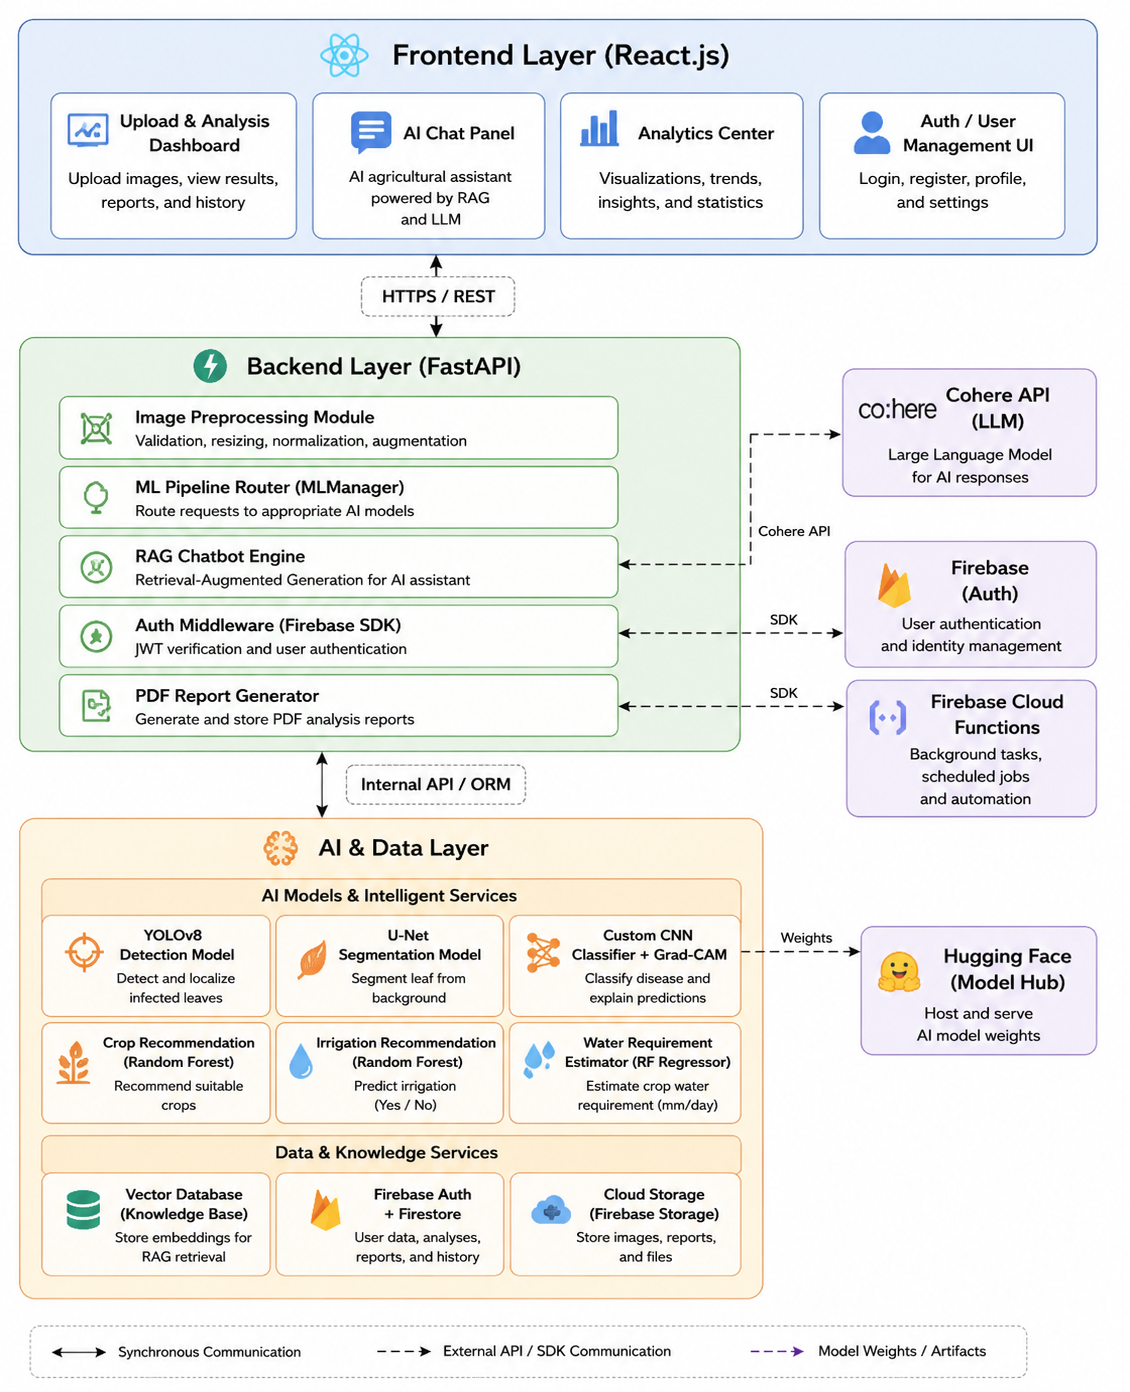
\includegraphics[width=\textwidth]{assets/diagrams/system_workflow.png}
\caption{Overall Workflow of the NABTA Platform}
\label{fig:system_workflow}
\end{figure}

The Presentation Layer consists of a React.js web application that provides users with interactive interfaces for plant disease analysis, irrigation prediction, crop recommendation, AI consultation, historical analysis, dashboard visualization, and account management.

The Application Layer is implemented using FastAPI, which acts as the central orchestration server. It manages user authentication, image preprocessing, request routing, communication with artificial intelligence models, report generation, database interaction, and external API integration.

The Artificial Intelligence Layer contains all deployed intelligent models used throughout the platform. These include the YOLOv8x object detector for infected leaf localization, the U-Net segmentation model with an EfficientNet-B0 encoder for leaf extraction, the custom CNN classifier for plant disease recognition, Grad-CAM for explainability and disease severity estimation, a Random Forest classifier for crop recommendation, a Random Forest classifier for irrigation decision prediction, and a Random Forest regressor for estimating crop water requirements.

The Cloud Data Layer integrates Firebase Authentication, Cloud Firestore, Firebase Cloud Functions, the Cohere API, Retrieval-Augmented Generation (RAG), and Hugging Face model hosting. These services collectively provide secure authentication, cloud data storage, conversational AI capabilities, document retrieval, and deployment of trained deep learning models.

This layered architecture enables loose coupling between software components, simplifies maintenance, improves scalability, and allows each subsystem to be updated independently without affecting the remaining parts of the platform.

%==============================================================================
\begin{figure}[H]
\centering
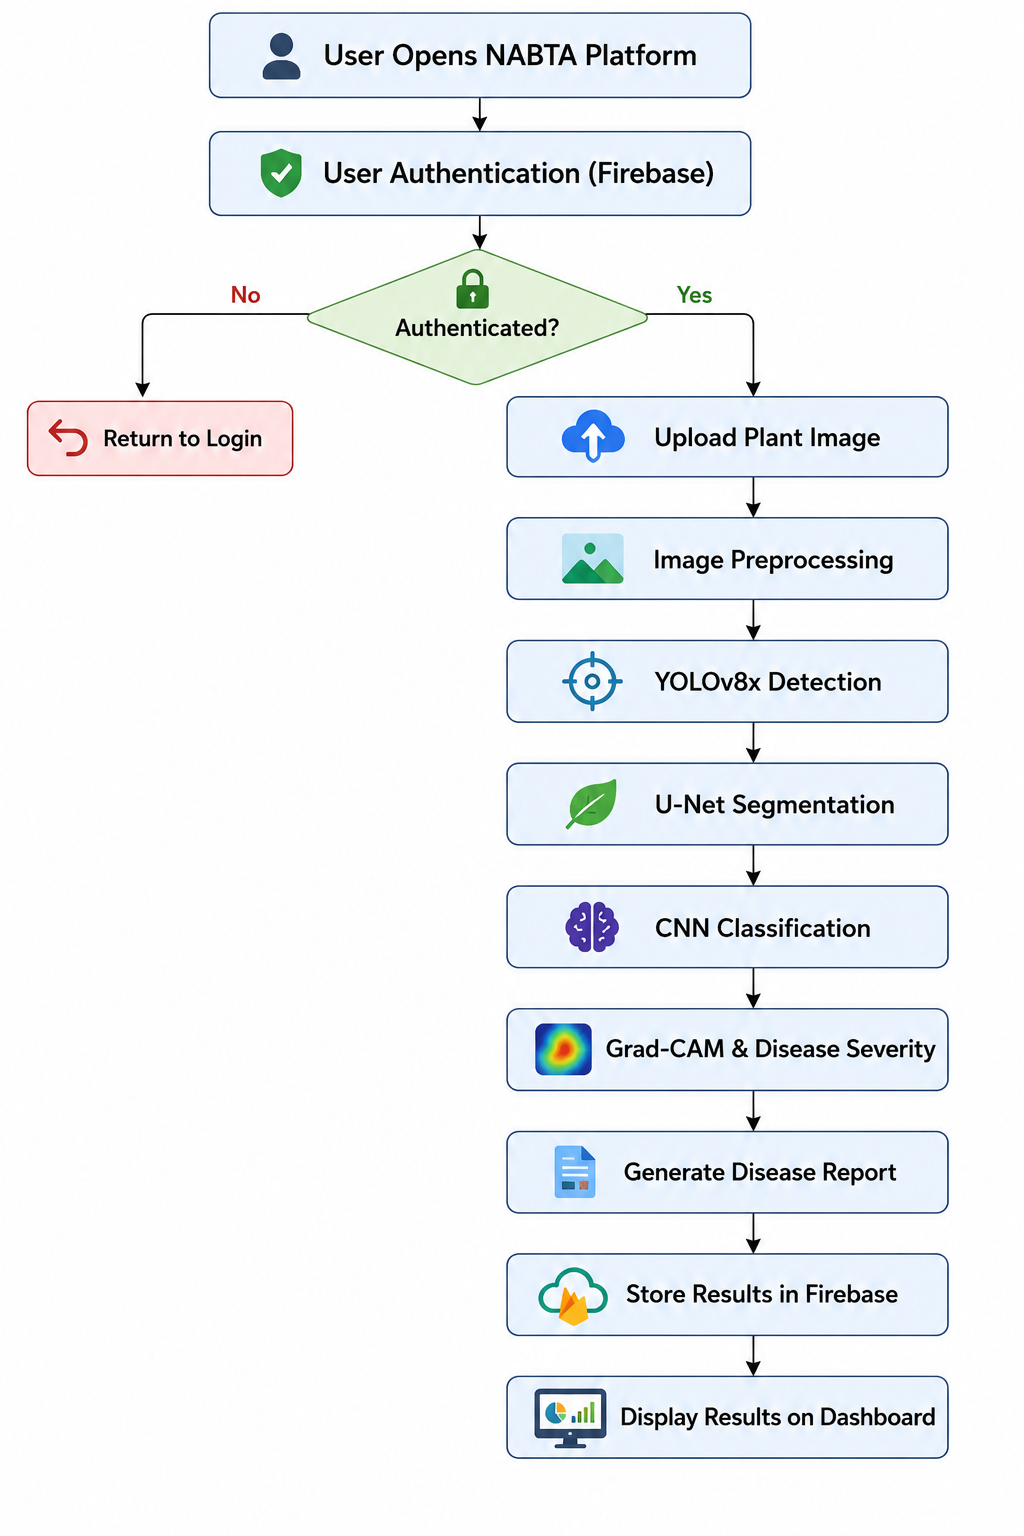
\includegraphics[width=0.85\textwidth]{assets/diagrams/system_workflows.png}
\caption{Overall Workflow of the NABTA Platform}
\label{fig:system_workflow}
\end{figure}

The execution process begins when a user accesses the web application through the React.js frontend. After successful authentication using Firebase Authentication, users can access the available intelligent services including plant disease analysis, crop recommendation, irrigation management, AI consultation, and historical records.

For plant disease diagnosis, the user uploads a leaf image through the Plant Analysis interface. The uploaded image is transmitted to the FastAPI backend, which performs image validation and preprocessing before initiating the artificial intelligence pipeline.

The AI pipeline executes four consecutive stages. First, the YOLOv8x model detects and localizes the infected leaf region. Second, the detected region is forwarded to the U-Net segmentation model, which separates the leaf from the surrounding background. Third, the segmented leaf image is analyzed by the custom CNN classifier to determine the plant species and disease category. Finally, Grad-CAM generates an explainability heatmap while simultaneously estimating disease severity based on the highlighted infected regions.

The generated results, including the detected disease, confidence score, segmentation mask, Grad-CAM visualization, and severity estimation, are stored in Cloud Firestore and displayed through the frontend interface. Users may also generate a PDF report containing the complete diagnosis.

The platform additionally provides two intelligent decision-support services. The crop recommendation module predicts the most suitable crops based on soil characteristics and environmental conditions, while the irrigation management module predicts irrigation requirements and estimates crop water demand using dedicated Random Forest models.

For agricultural consultation, user queries are processed through the Retrieval-Augmented Generation (RAG) pipeline. Relevant agricultural documents are first retrieved from the knowledge base before the query is forwarded to the Cohere Large Language Model, ensuring that generated responses remain domain-specific and evidence-based.

This workflow integrates multiple artificial intelligence techniques within a unified architecture while maintaining efficient communication between all system components.

%==============================================================================
\section{Use Case Diagram}
\label{sec:use_case}

The functional requirements of the NABTA platform are represented using the UML Use Case Diagram shown in Figure~\ref{fig:use_case}.

\begin{figure}[H]
\centering
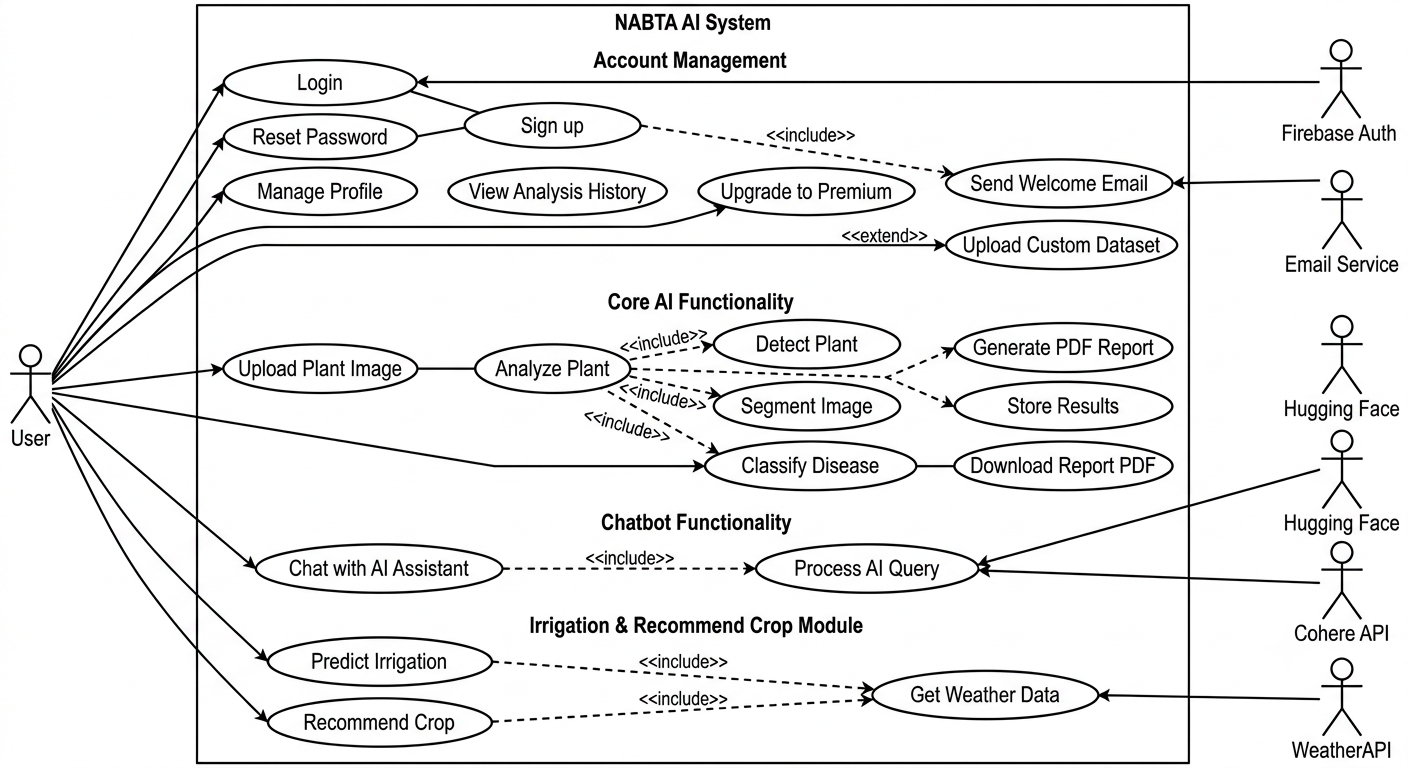
\includegraphics[width=\textwidth]{assets/diagrams/use_case_diagram.png}
\caption{Use Case Diagram of the NABTA Platform}
\label{fig:use_case}
\end{figure}

The system primarily interacts with two categories of actors:

\begin{itemize}
\item \textbf{User}, who utilizes the intelligent agricultural services.
\item \textbf{Administrator}, who manages system resources and user accounts.
\end{itemize}

External services including Firebase Authentication, Cohere API, Hugging Face, Weather API, and Email Services cooperate with the system to provide authentication, artificial intelligence inference, weather information, and notification services.

The User actor can perform the following operations:

\begin{itemize}
\item Register and authenticate.
\item Upload plant images.
\item Analyze plant diseases.
\item View disease reports.
\item Generate PDF reports.
\item Communicate with the AI Assistant.
\item Obtain crop recommendations.
\item Receive irrigation recommendations.
\item Browse previous analysis records.
\item View analytical dashboards.
\item Manage personal profile information.
\end{itemize}

The Administrator possesses additional privileges, including managing users, monitoring system status, maintaining agricultural datasets, and supervising platform resources.

The use case diagram demonstrates that all intelligent services are accessed through a unified interface while authentication and authorization mechanisms ensure secure access to protected resources.

%==============================================================================
\section{Activity Diagram}
\label{sec:activity_diagram}

The Activity Diagram illustrates the sequence of operations performed during the plant disease diagnosis process. It describes how user interactions trigger successive software components until the final diagnosis is produced.

Figure~\ref{fig:activity_diagram} presents the activity diagram of the proposed system.

\begin{figure}[H]
\centering
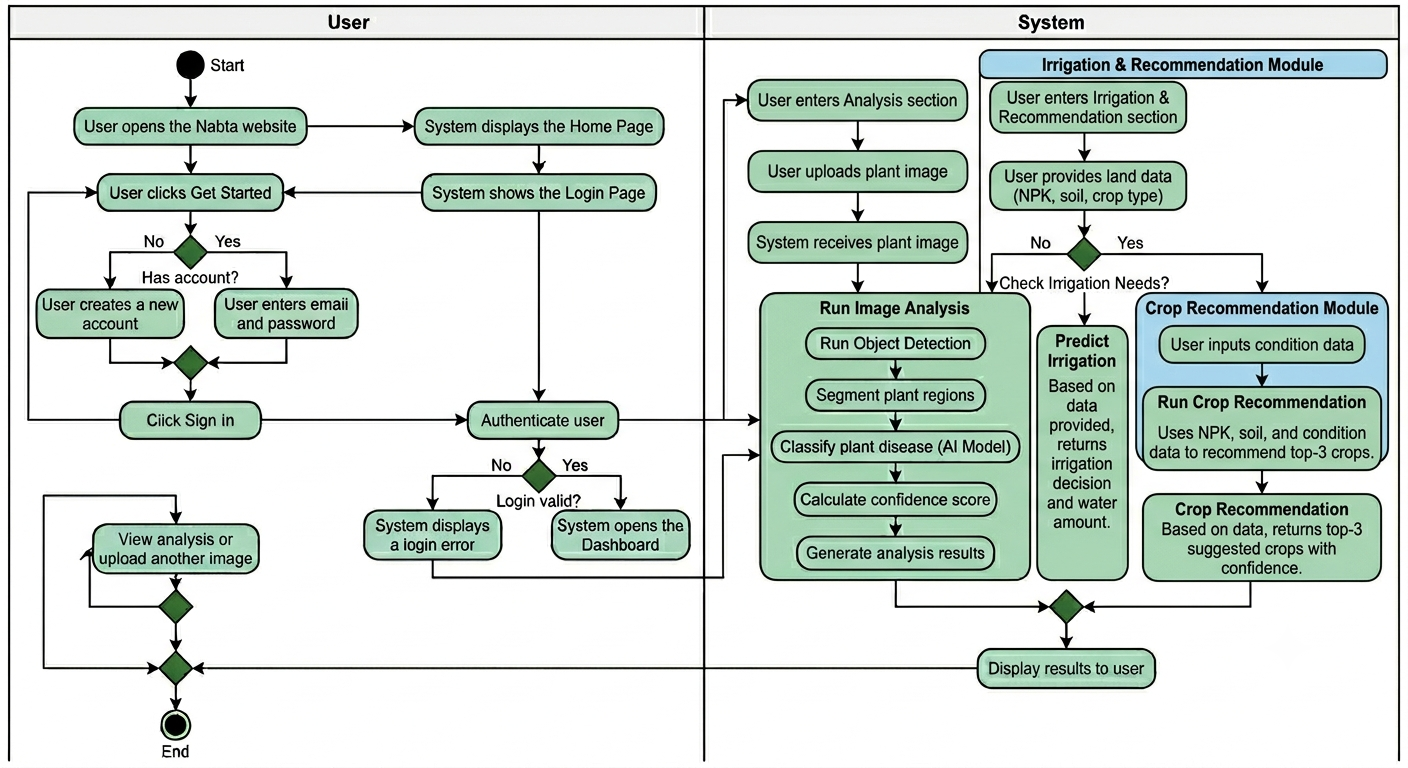
\includegraphics[width=.95\textwidth]{assets/diagrams/activity_diagram.png}
\caption{Activity Diagram of the Plant Disease Diagnosis Process}
\label{fig:activity_diagram}
\end{figure}

The workflow begins when the user uploads a plant image through the web interface. The backend validates the uploaded image before forwarding it to the artificial intelligence pipeline.

The YOLOv8x detector first localizes the infected leaf region. The cropped image is then processed by the U-Net segmentation model to isolate the leaf from the background. The segmented image is subsequently classified using the CNN model, which predicts one of the supported plant disease classes.

Grad-CAM generates an explainability heatmap and estimates disease severity. Finally, the diagnosis report is generated, stored in Firebase Cloud Firestore, and presented to the user through the frontend interface.

This sequential workflow minimizes unnecessary computations while ensuring that every stage receives optimized input from the previous model.

%==============================================================================
\section{Sequence Diagram}
\label{sec:sequence_diagram}

The Sequence Diagram describes the interactions among the user, frontend application, backend services, artificial intelligence models, and cloud infrastructure during a typical disease diagnosis session.

Figure~\ref{fig:sequence_diagram} illustrates these interactions.

\begin{figure}[H]
\centering
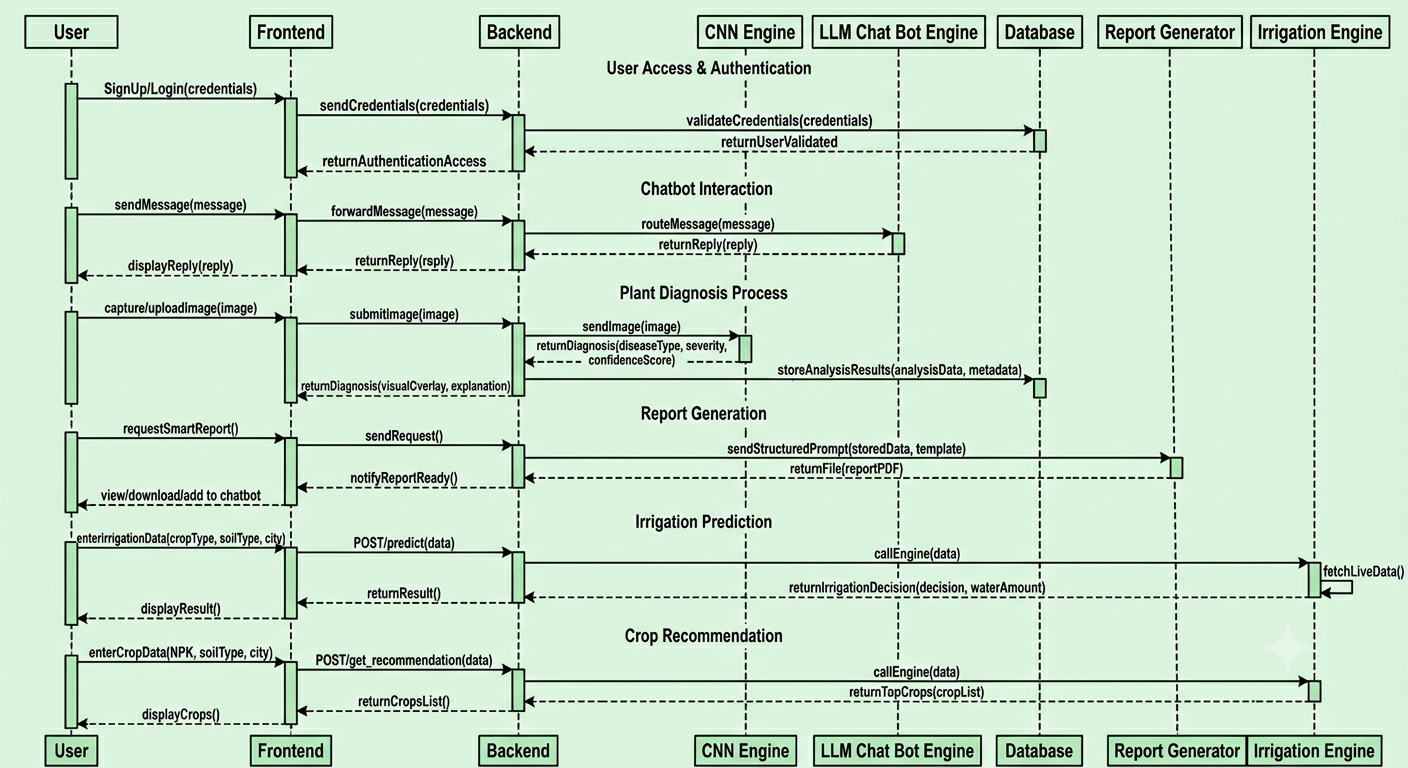
\includegraphics[width=\textwidth]{assets/diagrams/sequence_diagram.png}
\caption{Sequence Diagram of the NABTA Platform}
\label{fig:sequence_diagram}
\end{figure}

The interaction begins when the user uploads a plant image through the React.js frontend. The frontend transmits the image to the FastAPI backend, which performs validation before initiating the AI pipeline.

The backend sequentially invokes the YOLOv8x detection model, the U-Net segmentation model, and the CNN classifier. Once classification is completed, Grad-CAM generates the explainability visualization and disease severity estimation.

The generated diagnosis is stored in Cloud Firestore, while optional PDF reports are produced upon user request.

When agricultural consultation is requested, the backend retrieves relevant knowledge through the Retrieval-Augmented Generation (RAG) pipeline before forwarding the enriched prompt to the Cohere Large Language Model.

Finally, all generated outputs are returned to the frontend and displayed through the user interface.

%==============================================================================
\section{Class Diagram}
\label{sec:class_diagram}

The object-oriented structure of the software system is represented using the UML Class Diagram shown in Figure~\ref{fig:class_diagram}.

\begin{figure}[H]
\centering
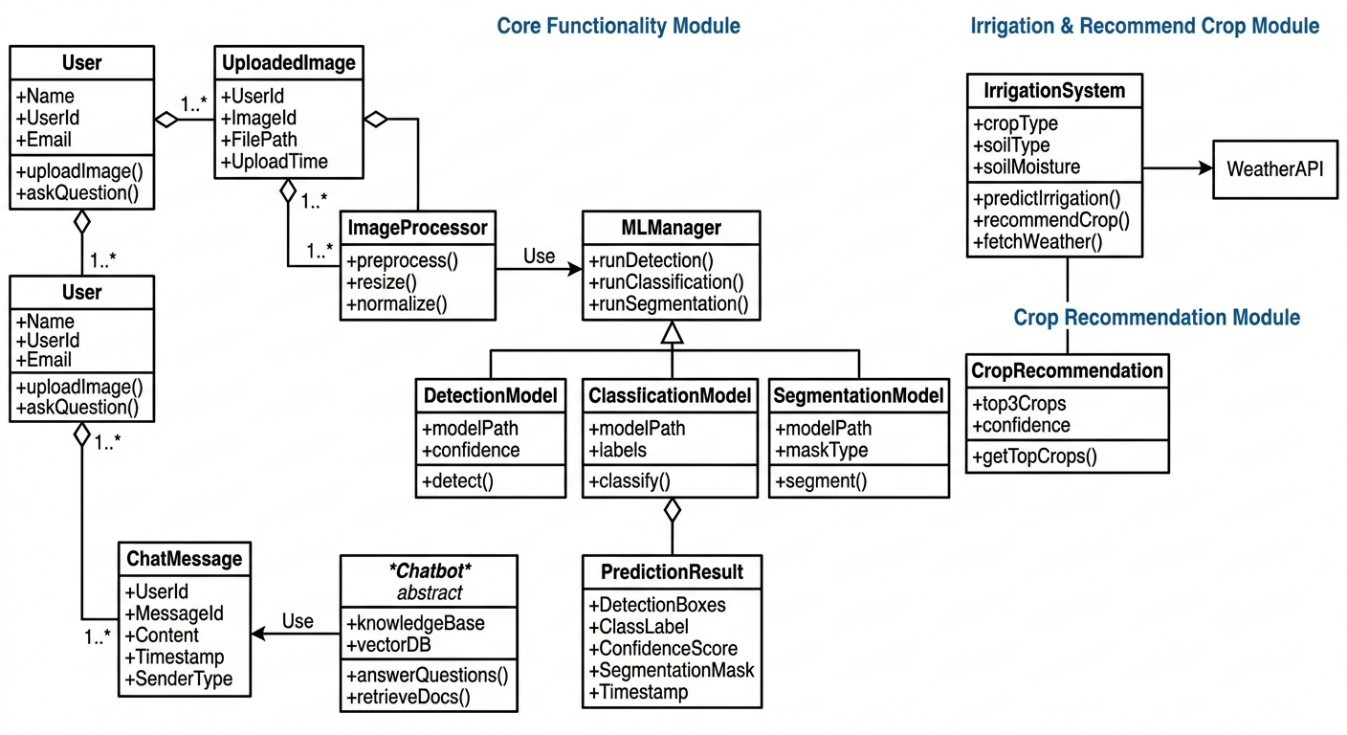
\includegraphics[width=\textwidth]{assets/diagrams/class_diagram.png}
\caption{Class Diagram of the NABTA Platform}
\label{fig:class_diagram}
\end{figure}

The system is composed of multiple logical classes responsible for user management, plant analysis, disease reports, chatbot interaction, crop recommendation, irrigation prediction, and report generation.

Relationships between these classes improve modularity while supporting future extensibility and maintainability.

Each software component encapsulates its own responsibilities, reducing coupling and improving software quality.

%==============================================================================
\section{Entity Relationship Diagram}
\label{sec:erd}

The persistent data used by the NABTA platform are stored in Google Cloud Firestore. Although Firestore is a NoSQL document-oriented database, the logical relationships between the major entities can still be represented using an Entity Relationship Diagram (ERD).

Figure~\ref{fig:erd} illustrates the logical data model adopted in the proposed platform.

\begin{figure}[H]
\centering
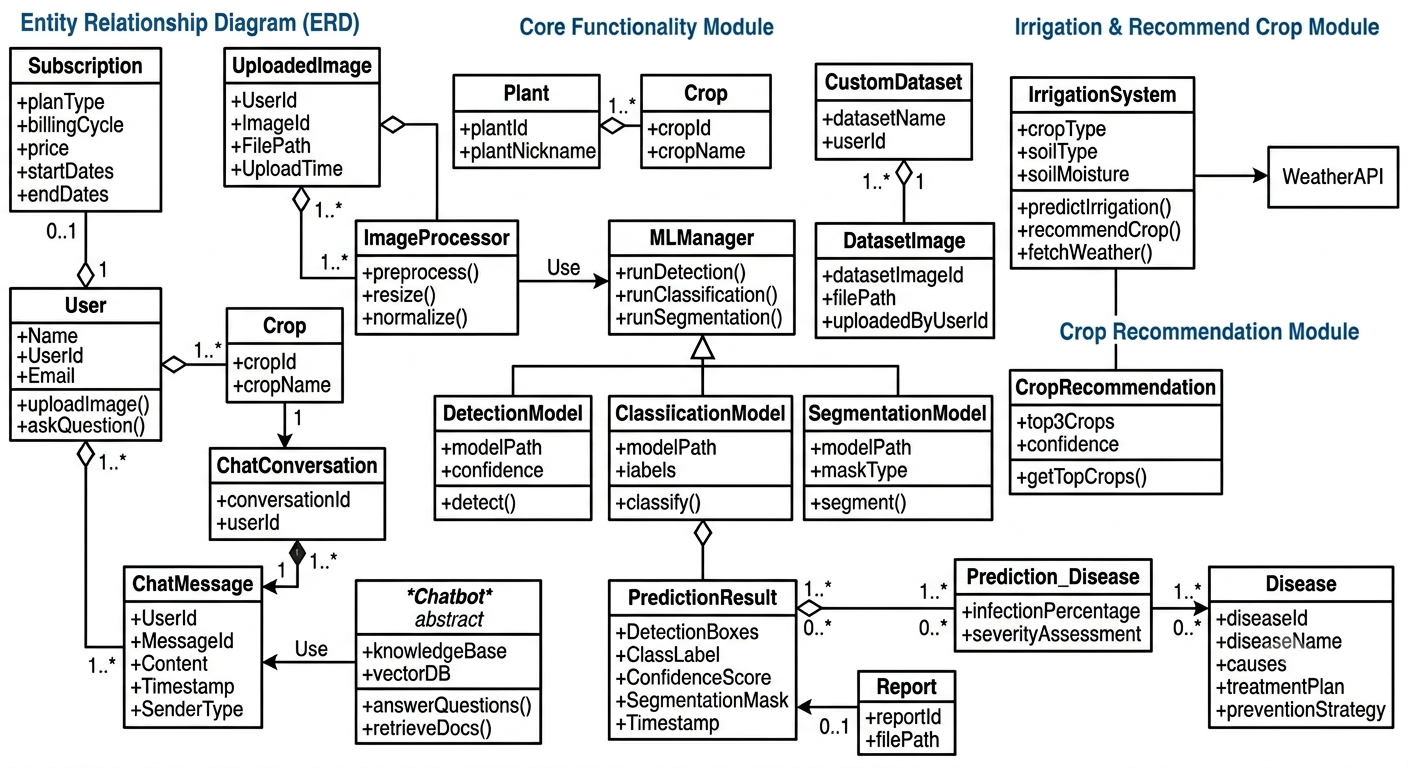
\includegraphics[width=.95\textwidth]{assets/diagrams/entity_relationship_diagram.png}
\caption{Entity Relationship Diagram of the NABTA Platform}
\label{fig:erd}
\end{figure}

The database is organized around several primary entities that store user information, plant disease analyses, chatbot conversations, recommendation records, and generated reports.

The main entities include:

\begin{itemize}

\item Users

\item Plant Analysis

\item Disease Reports

\item Chat History

\item Crop Recommendations

\item Irrigation Records

\item PDF Reports

\item Custom Dataset

\end{itemize}

Each authenticated user may own multiple disease analyses, recommendation records, chatbot conversations, and generated reports, allowing the platform to maintain a complete history of agricultural activities.

The document-oriented design of Cloud Firestore provides high scalability, low latency, and seamless synchronization with the frontend application.

%==============================================================================
\section{Database Design}
\label{sec:database_design}

The NABTA platform utilizes Firebase Cloud Firestore as its primary cloud database. Firestore stores information as collections of JSON-like documents, enabling flexible schema evolution while supporting real-time synchronization.

The major collections implemented in the platform are summarized in Table~\ref{tab:firestore_collections}.

\begin{table}[H]
\centering
\caption{Firestore Collections}
\label{tab:firestore_collections}
\renewcommand{\arraystretch}{1.35}

\begin{tabularx}{\textwidth}{>{\raggedright\arraybackslash}p{4cm}X}

\toprule

\textbf{Collection} &
\textbf{Description}

\\

\midrule

Users &
Stores user account information, authentication identifiers, profile details, and subscription information.

\\

PlantAnalysis &
Stores uploaded images, disease predictions, confidence scores, Grad-CAM visualizations, and disease severity estimations.

\\

DiseaseReports &
Stores generated disease diagnosis reports and treatment recommendations.

\\

ChatHistory &
Stores conversations between users and the AI agricultural assistant.

\\

CropRecommendations &
Stores crop recommendation requests together with predicted crops and confidence values.

\\

IrrigationRecords &
Stores irrigation prediction requests, irrigation decisions, and estimated crop water requirements.

\\

PDFReports &
Stores metadata associated with generated PDF reports.

\\

CustomDataset &
Stores administrator-managed agricultural knowledge and user-defined records.

\\

\bottomrule

\end{tabularx}

\end{table}

Each document is uniquely identified using Firebase-generated document identifiers. Relationships between documents are maintained using user identifiers and analysis identifiers, enabling efficient retrieval of historical records without introducing unnecessary data duplication.

The adopted database design supports horizontal scalability while maintaining high availability and low response latency.

%==============================================================================
\subsection{Database Relationships}

Although Firestore is a document-oriented database, logical relationships exist between the stored collections.

A single user may perform multiple plant analyses, generate multiple PDF reports, communicate with the AI assistant several times, and request both irrigation and crop recommendations.

The principal relationships are summarized below:

\begin{itemize}

\item One User $\rightarrow$ Many Plant Analysis Records

\item One User $\rightarrow$ Many Disease Reports

\item One User $\rightarrow$ Many Chat Conversations

\item One User $\rightarrow$ Many Crop Recommendations

\item One User $\rightarrow$ Many Irrigation Records

\item One User $\rightarrow$ Many PDF Reports

\end{itemize}

This logical organization simplifies historical record retrieval while maintaining data consistency throughout the platform.

%==============================================================================
\section{Component Diagram}
\label{sec:component_diagram}

The Component Diagram illustrates the modular organization of the NABTA platform and the interactions among its major software components.

Figure~\ref{fig:component_diagram} presents the component architecture adopted in the proposed system.

\begin{figure}[H]
\centering
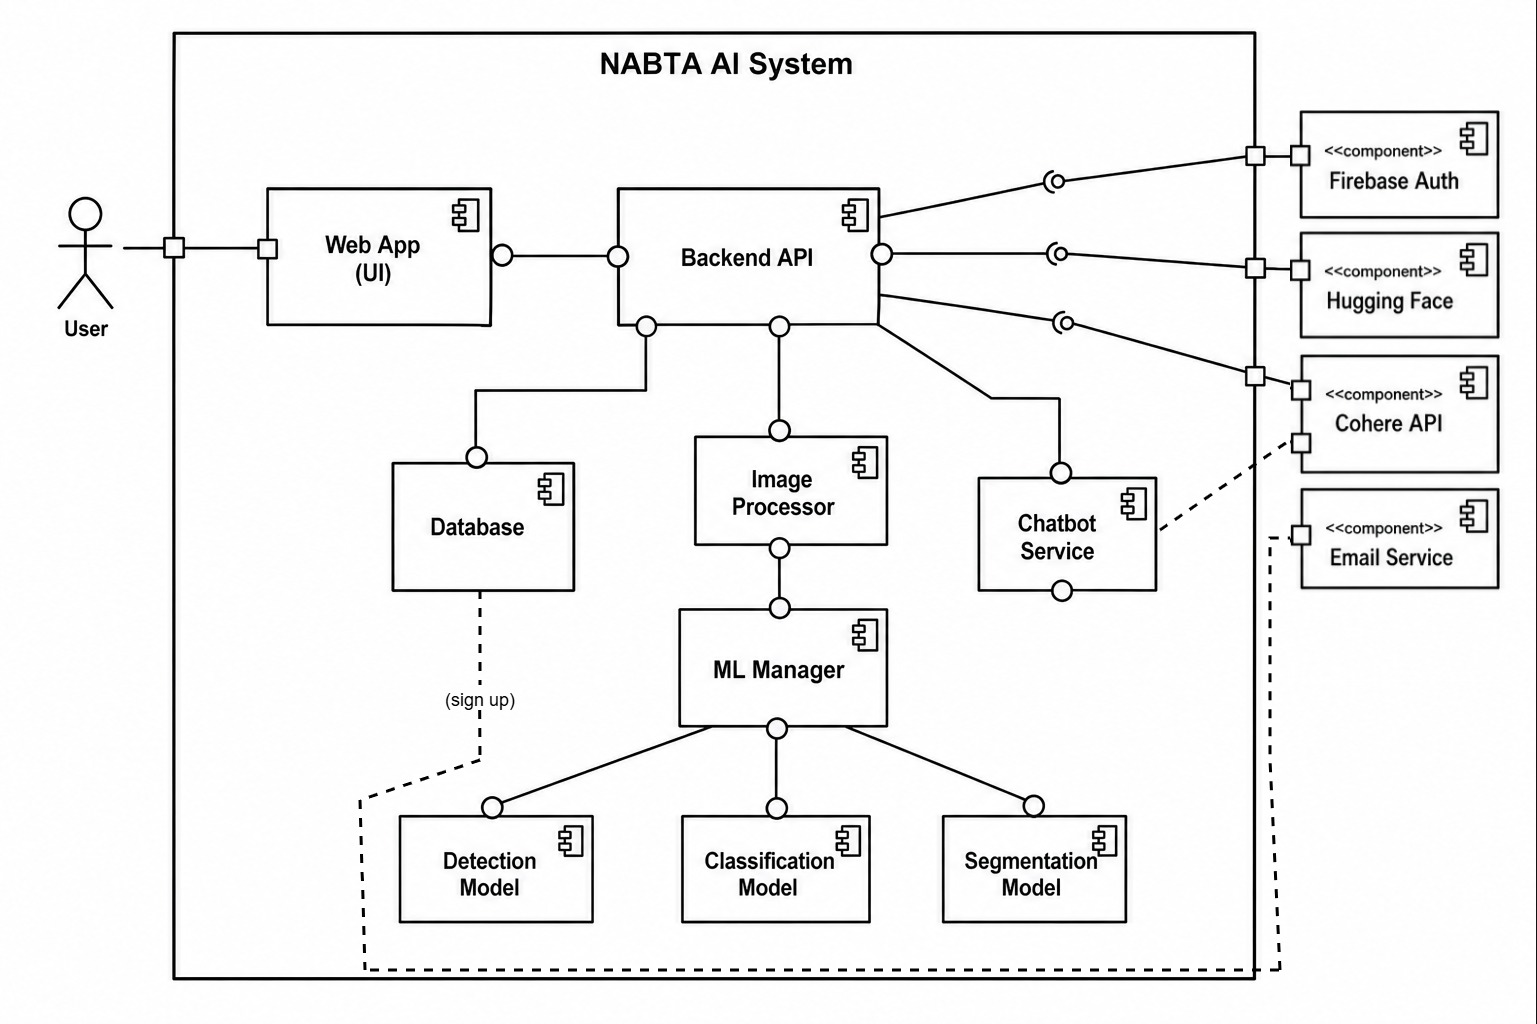
\includegraphics[width=\textwidth]{assets/diagrams/component_diagram.jpeg}
\caption{Component Diagram of the NABTA Platform}
\label{fig:component_diagram}
\end{figure}

The platform consists of several independent but interconnected software components, each responsible for a specific functionality.

The major components include:

\begin{itemize}

\item React.js Frontend

\item FastAPI Backend

\item Authentication Service

\item Plant Disease Analysis Service

\item YOLOv8x Detection Service

\item U-Net Segmentation Service

\item CNN Classification Service

\item Grad-CAM Explainability Service

\item Crop Recommendation Service

\item Irrigation Recommendation Service

\item AI Assistant Service

\item PDF Report Generator

\item Firebase Cloud Services

\item Cloud Firestore Database

\end{itemize}

The modular architecture allows every component to operate independently while communicating through RESTful APIs. Such separation simplifies future maintenance, testing, and deployment.

%==============================================================================
\section{Deployment Diagram}
\label{sec:deployment}

The Deployment Diagram illustrates how software components are distributed across cloud infrastructure and client devices.

Figure~\ref{fig:deployment_diagram} presents the deployment architecture of NABTA.

\begin{figure}[H]
\centering
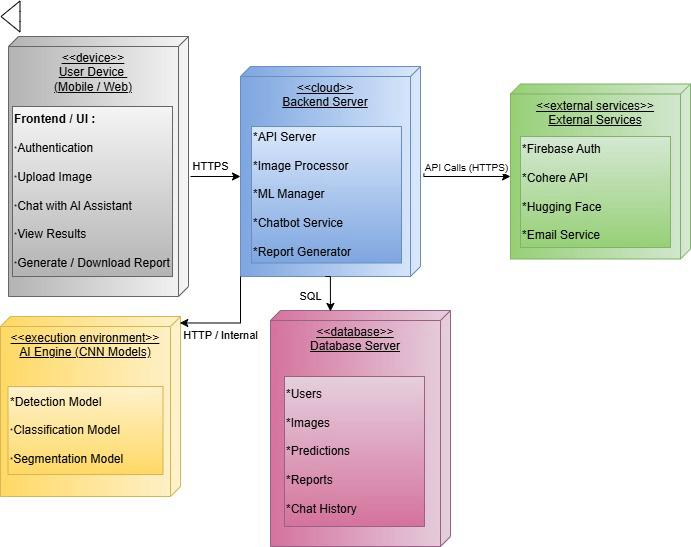
\includegraphics[width=\textwidth]{assets/diagrams/deployment_diagram.jpeg}
\caption{Deployment Diagram of the NABTA Platform}
\label{fig:deployment_diagram}
\end{figure}

The deployment architecture consists of four major nodes:

\begin{enumerate}

\item Client Device

\item Frontend Server

\item Backend Server

\item Cloud Services

\end{enumerate}

Users access the platform through modern web browsers. The React.js application communicates with the FastAPI backend using HTTPS requests.

The backend performs AI inference by invoking the deployed computer vision and machine learning models. Firebase Authentication verifies user identities, while Cloud Firestore stores persistent application data.

The Cohere API is responsible for generating intelligent conversational responses through the Retrieval-Augmented Generation (RAG) pipeline, whereas Hugging Face hosts the deployed deep learning inference services.

This deployment strategy provides scalability, security, and efficient resource utilization.

%==============================================================================
\section{REST API Design}
\label{sec:api_design}

Communication between the frontend application and backend services is performed through RESTful APIs implemented using FastAPI.

Each API endpoint performs a dedicated task while exchanging data in JSON format.

Table~\ref{tab:api_endpoints} summarizes the principal REST API endpoints implemented in the NABTA platform.

\begin{table}[H]
\centering
\caption{Main REST API Endpoints}
\label{tab:api_endpoints}
\renewcommand{\arraystretch}{1.35}

\begin{tabularx}{\textwidth}{>{\raggedright\arraybackslash}p{4cm}>{\raggedright\arraybackslash}p{3cm}X}

\toprule

\textbf{Endpoint} &
\textbf{Method} &
\textbf{Purpose}

\\

\midrule

/api/detect &
POST &
Detect infected leaf using YOLOv8x.

\\

/api/segment &
POST &
Generate the leaf segmentation mask.

\\

/api/classify &
POST &
Predict plant species and disease class.

\\

/api/analyze &
POST &
Execute the complete AI analysis pipeline.

\\

/api/chat &
POST &
Generate AI agricultural consultation.

\\

/api/crop-recommendation &
POST &
Recommend suitable crops.

\\

/api/irrigation &
POST &
Predict irrigation decision.

\\

/api/water-requirement &
POST &
Estimate crop water requirement.

\\

/api/report &
POST &
Generate PDF disease reports.

\\

/api/history &
GET &
Retrieve previous analysis records.

\\

/api/profile &
GET &
Retrieve user profile information.

\\

\bottomrule

\end{tabularx}

\end{table}

The REST architecture enables loose coupling between the frontend and backend while allowing individual services to evolve independently. FastAPI automatically generates OpenAPI documentation, simplifying API testing and future integration with external applications.

%==============================================================================
\section{Security Architecture}
\label{sec:security}

Security represents one of the fundamental design considerations of the NABTA platform. Since the system processes user accounts, uploaded plant images, historical records, and artificial intelligence services, multiple security mechanisms were incorporated throughout the system architecture.

The proposed security framework consists of several complementary layers that collectively protect user information, backend services, and cloud resources.

\subsection{Authentication and Authorization}

User authentication is managed through Firebase Authentication using secure email and password credentials.

After successful authentication, Firebase generates a JSON Web Token (JWT) that accompanies every protected request sent to the backend. The FastAPI server validates this token before granting access to secured endpoints, ensuring that only authenticated users can utilize protected platform services.

Role-based authorization is also supported, allowing administrators to access management functions while restricting regular users to their own resources.

\subsection{Secure API Communication}

All communication between the frontend and backend is performed through HTTPS using encrypted TLS connections.

The backend validates every incoming request before processing, including:

\begin{itemize}

\item Authentication token verification.

\item Uploaded image validation.

\item Input parameter validation.

\item File type verification.

\item Request size limitation.

\end{itemize}

These validation mechanisms reduce the risk of malformed requests and unauthorized access.

\subsection{API Key Protection}

Sensitive credentials such as the Cohere API key, Firebase configuration, and external service tokens are never embedded directly within the frontend application.

Instead, all confidential information is stored securely using environment variables on the backend server. This prevents accidental exposure of credentials while simplifying deployment across different environments.

\subsection{Cloud Security}

Firebase Authentication and Cloud Firestore implement multiple built-in security mechanisms including encrypted communication, access control rules, and user-based authorization.

Firestore security rules ensure that users can access only their own analysis records, generated reports, and chatbot conversations.

These cloud-level protections significantly improve overall platform security without increasing implementation complexity.

%==============================================================================
\section{Design Principles}
\label{sec:design_principles}

Several software engineering principles guided the design of the proposed NABTA platform.

\begin{itemize}

\item \textbf{Modularity}

Each intelligent component operates as an independent service with clearly defined responsibilities.

\item \textbf{Scalability}

The architecture allows additional artificial intelligence models or cloud services to be integrated without major structural modifications.

\item \textbf{Maintainability}

Independent software modules simplify debugging, testing, maintenance, and future system upgrades.

\item \textbf{Reusability}

Reusable frontend components and backend APIs reduce software duplication while improving development efficiency.

\item \textbf{Loose Coupling}

RESTful communication minimizes dependencies between the frontend, backend, artificial intelligence models, and cloud services.

\item \textbf{High Cohesion}

Each module performs one primary responsibility, resulting in improved software quality and readability.

\end{itemize}

Applying these principles resulted in a flexible architecture capable of supporting future expansion while maintaining high software quality.

%==============================================================================
\section{Design Decisions}
\label{sec:design_decisions}

Several important architectural decisions were made during the development of NABTA.

React.js was selected for frontend development because of its component-based architecture, excellent performance, and extensive ecosystem.

FastAPI was adopted as the backend framework due to its asynchronous request handling, automatic API documentation, and high inference performance.

YOLOv8x was selected for object detection because it achieved superior localization accuracy compared with smaller YOLO variants.

U-Net with an EfficientNet-B0 encoder was chosen for semantic segmentation because it provides an excellent balance between segmentation accuracy and computational efficiency.

The disease classification module employs a custom CNN specifically designed for large-scale plant disease recognition across 102 classes.

Random Forest was selected for crop recommendation and irrigation prediction because it demonstrated strong predictive performance, robustness against overfitting, and excellent generalization capability.

Firebase provides authentication, cloud storage, and backend services, while Cohere and Retrieval-Augmented Generation enable intelligent agricultural consultation with improved factual consistency.

Collectively, these design decisions resulted in a scalable, maintainable, and production-ready smart agriculture platform.

%==============================================================================
\section{Chapter Summary}
\label{sec:chapter4_summary}

This chapter presented the complete architectural design of the NABTA smart agriculture platform.

The overall system architecture, execution workflow, UML diagrams, database structure, deployment strategy, REST API architecture, and security mechanisms were discussed in detail. Furthermore, the chapter described the software engineering principles and architectural decisions that guided the implementation of the platform.

The proposed design provides a modular, scalable, secure, and maintainable foundation that supports the integration of multiple artificial intelligence models within a unified web-based application.

The following chapter presents the implementation details of the developed system, including the frontend interfaces, backend services, artificial intelligence integration, cloud deployment, and user interaction.

%==============================================================================
% CHAPTER 5 --- SYSTEM IMPLEMENTATION
%==============================================================================

\chapter{System Implementation}
\label{chap:implementation}

\chapterquote{The best designs are those that successfully become working systems.}{Alan Kay}

%==============================================================================
\section{Overview}
\label{sec:implementation_overview}

This chapter presents the implementation details of the proposed NABTA platform. Following the system methodology presented in Chapter~3 and the architectural design described in Chapter~5, this chapter demonstrates how the proposed solution was transformed into a fully functional smart agriculture platform.

The implementation integrates modern web technologies, deep learning models, machine learning algorithms, cloud services, and explainable artificial intelligence within a unified production-ready application. The platform consists of a React.js frontend, a FastAPI backend, multiple AI models for image analysis and agricultural recommendation, Firebase cloud services, and a Retrieval-Augmented Generation (RAG) chatbot powered by the Cohere API.

The implementation workflow follows the same sequence adopted by the deployed system. First, the graphical user interfaces are presented, followed by the backend implementation, AI model integration, cloud services, and finally the complete system workflow.

%==============================================================================
\section{Frontend Implementation}
\label{sec:frontend}

The frontend of NABTA was implemented using React.js as a Single-Page Application (SPA). The interface was designed to provide an intuitive user experience while supporting complex AI functionalities through a modern dashboard-based design.

Responsive layouts, reusable components, dark/light themes, interactive visualizations, and asynchronous communication with the backend enable users to access all platform services through a unified interface.

The following subsections present the main user interfaces implemented in the system.

%==============================================================================
\subsection{Home Page}
\label{subsec:landing}

The landing page serves as the public entry point to the NABTA platform. It introduces the objectives of the system, highlights the available artificial intelligence services, and provides quick access to authentication and analysis modules.

The page presents the major capabilities of the platform, including plant disease diagnosis, crop recommendation, irrigation management, AI-powered consultation, and analytical dashboards. Modern animations and responsive design techniques were adopted to improve usability across desktop and mobile devices.

\begin{figure}[H]
\centering
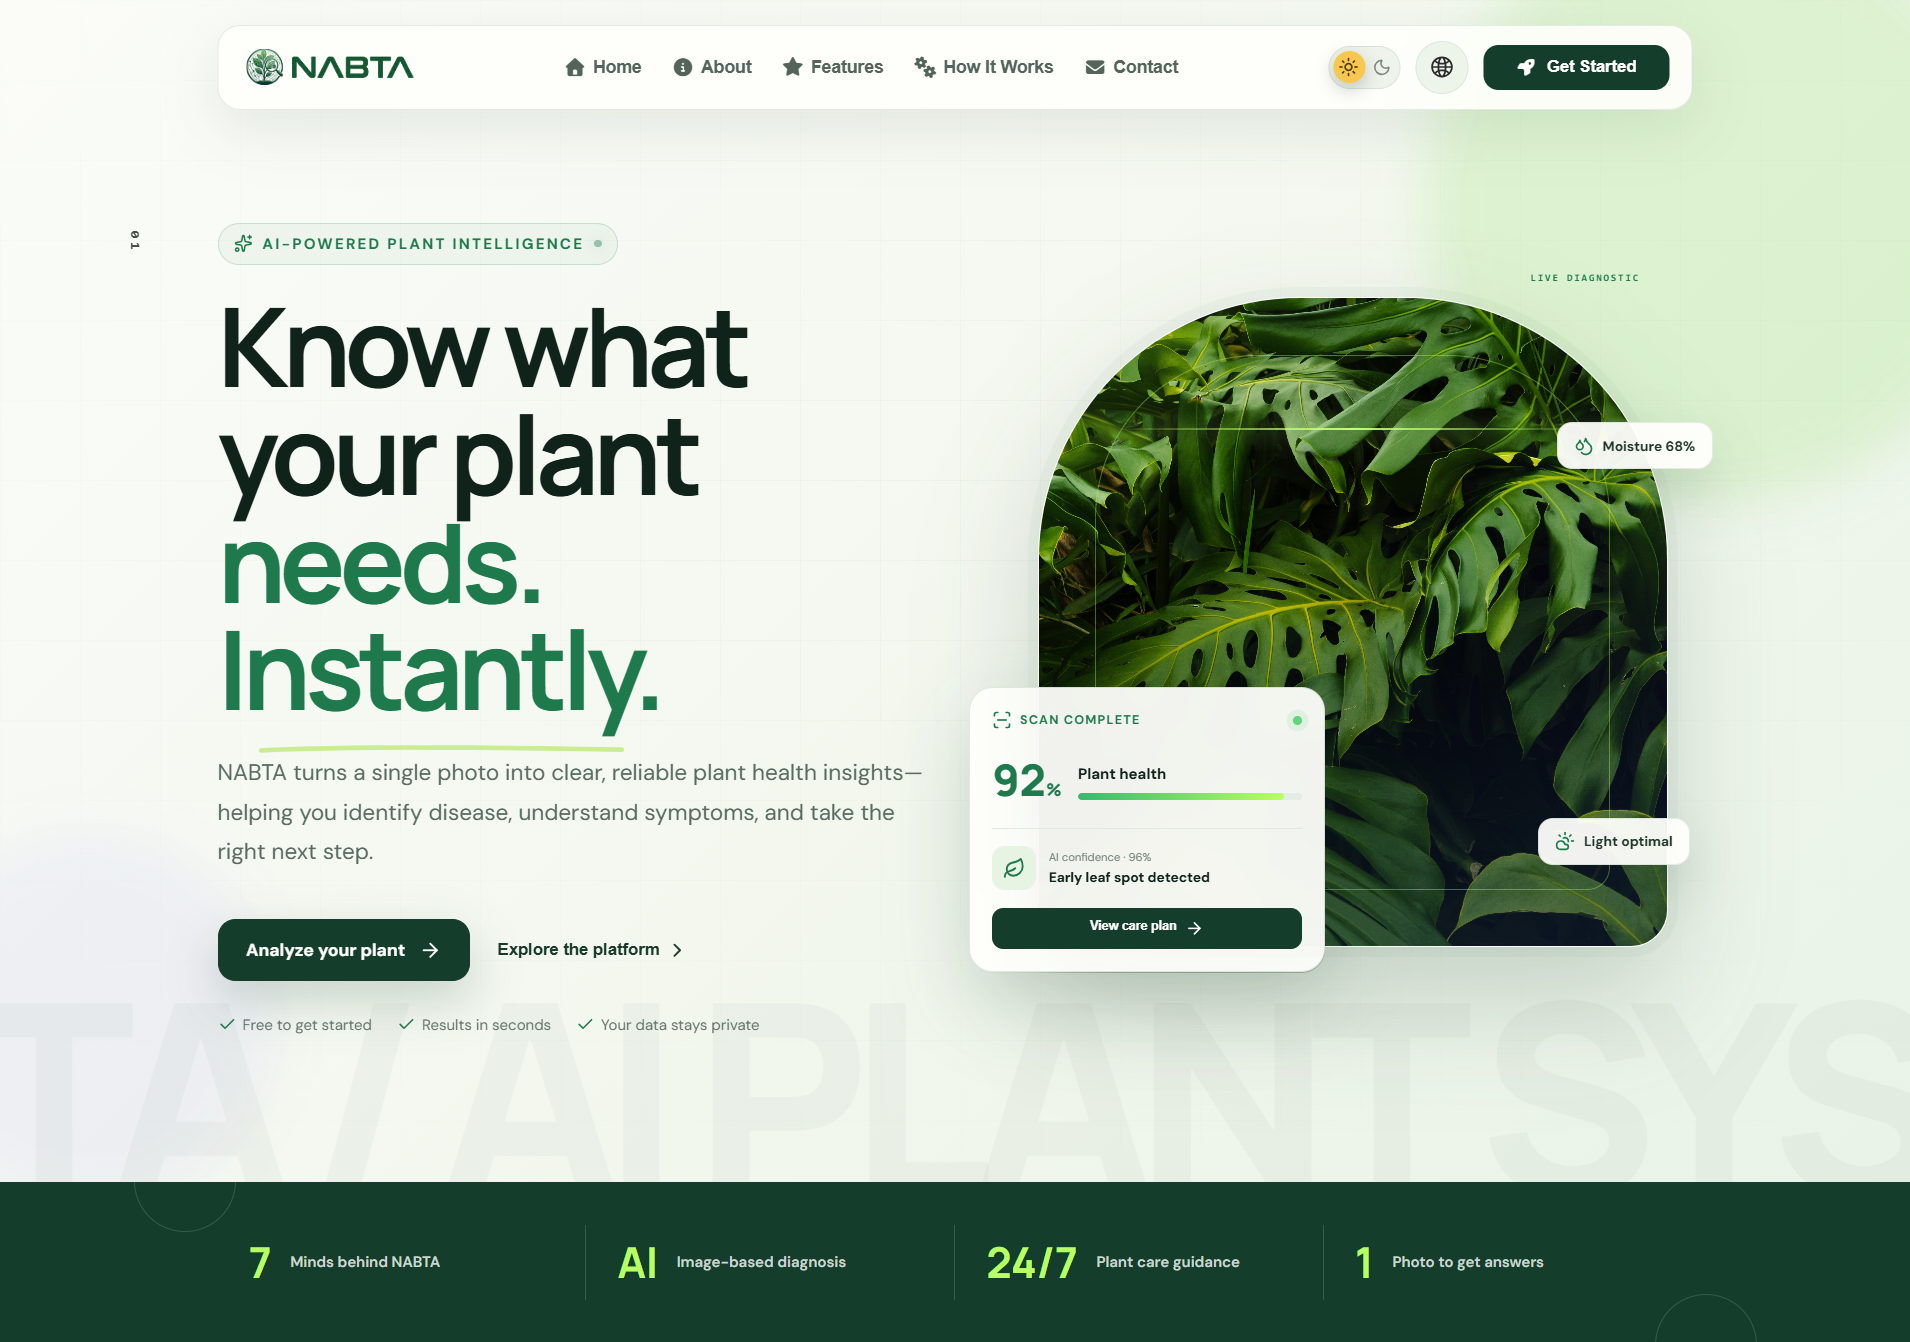
\includegraphics[width=\textwidth]{assets/screenshots/home_page.png}
\caption{NABTA Landing Page}
\label{fig:landing_page}
\end{figure}

%==============================================================================
\subsection{User Authentication}
\label{subsec:login}

User authentication is implemented using Firebase Authentication, providing secure account management through email and password authentication.

The authentication interface validates user credentials before granting access to protected platform features. Authentication tokens are securely generated by Firebase and verified by the FastAPI backend before processing any authorized request.

The login page also provides direct navigation to account registration and password recovery services.

\begin{figure}[H]
\centering
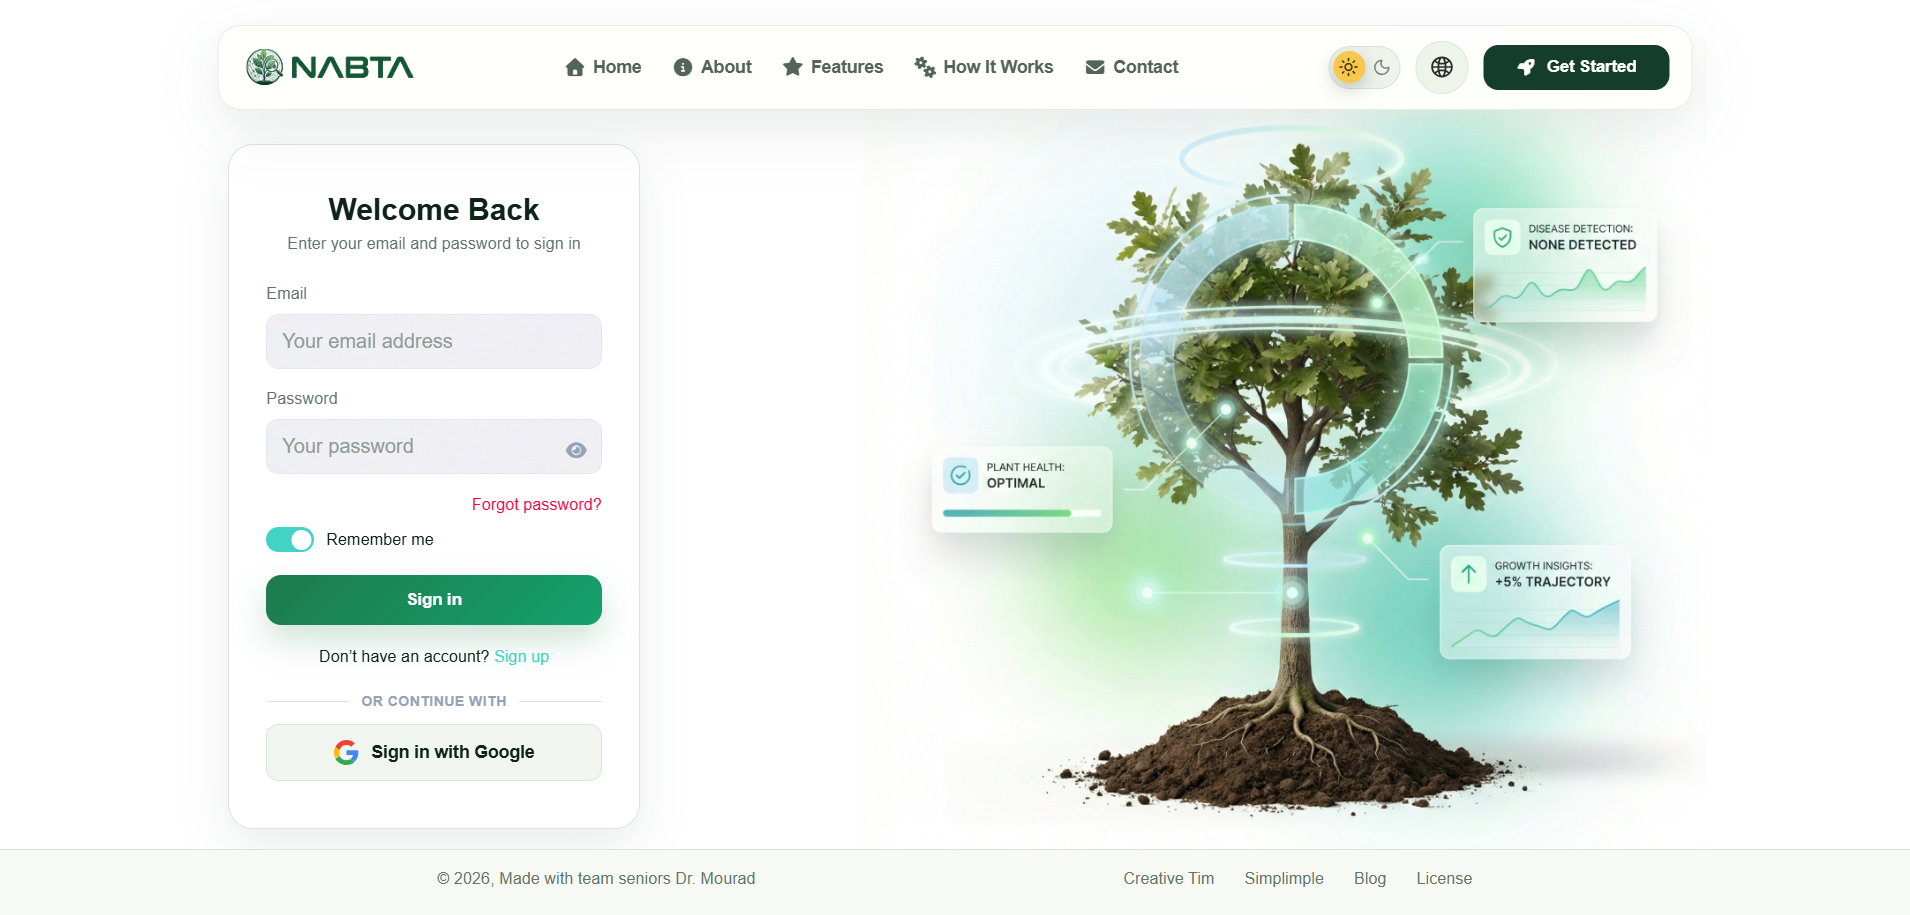
\includegraphics[width=.9\textwidth]{assets/screenshots/login_page.png}
\caption{User Authentication Interface}
\label{fig:login_page}
\end{figure}

%==============================================================================
\subsection{Password Recovery}
\label{subsec:reset_password}

To improve usability and account security, NABTA provides a password recovery mechanism integrated with Firebase Authentication.

Users can request a password reset by entering their registered email address. A secure password reset link is then sent automatically, allowing users to create a new password without administrator intervention.

This functionality improves accessibility while maintaining secure account management practices.

\begin{figure}[H]
\centering
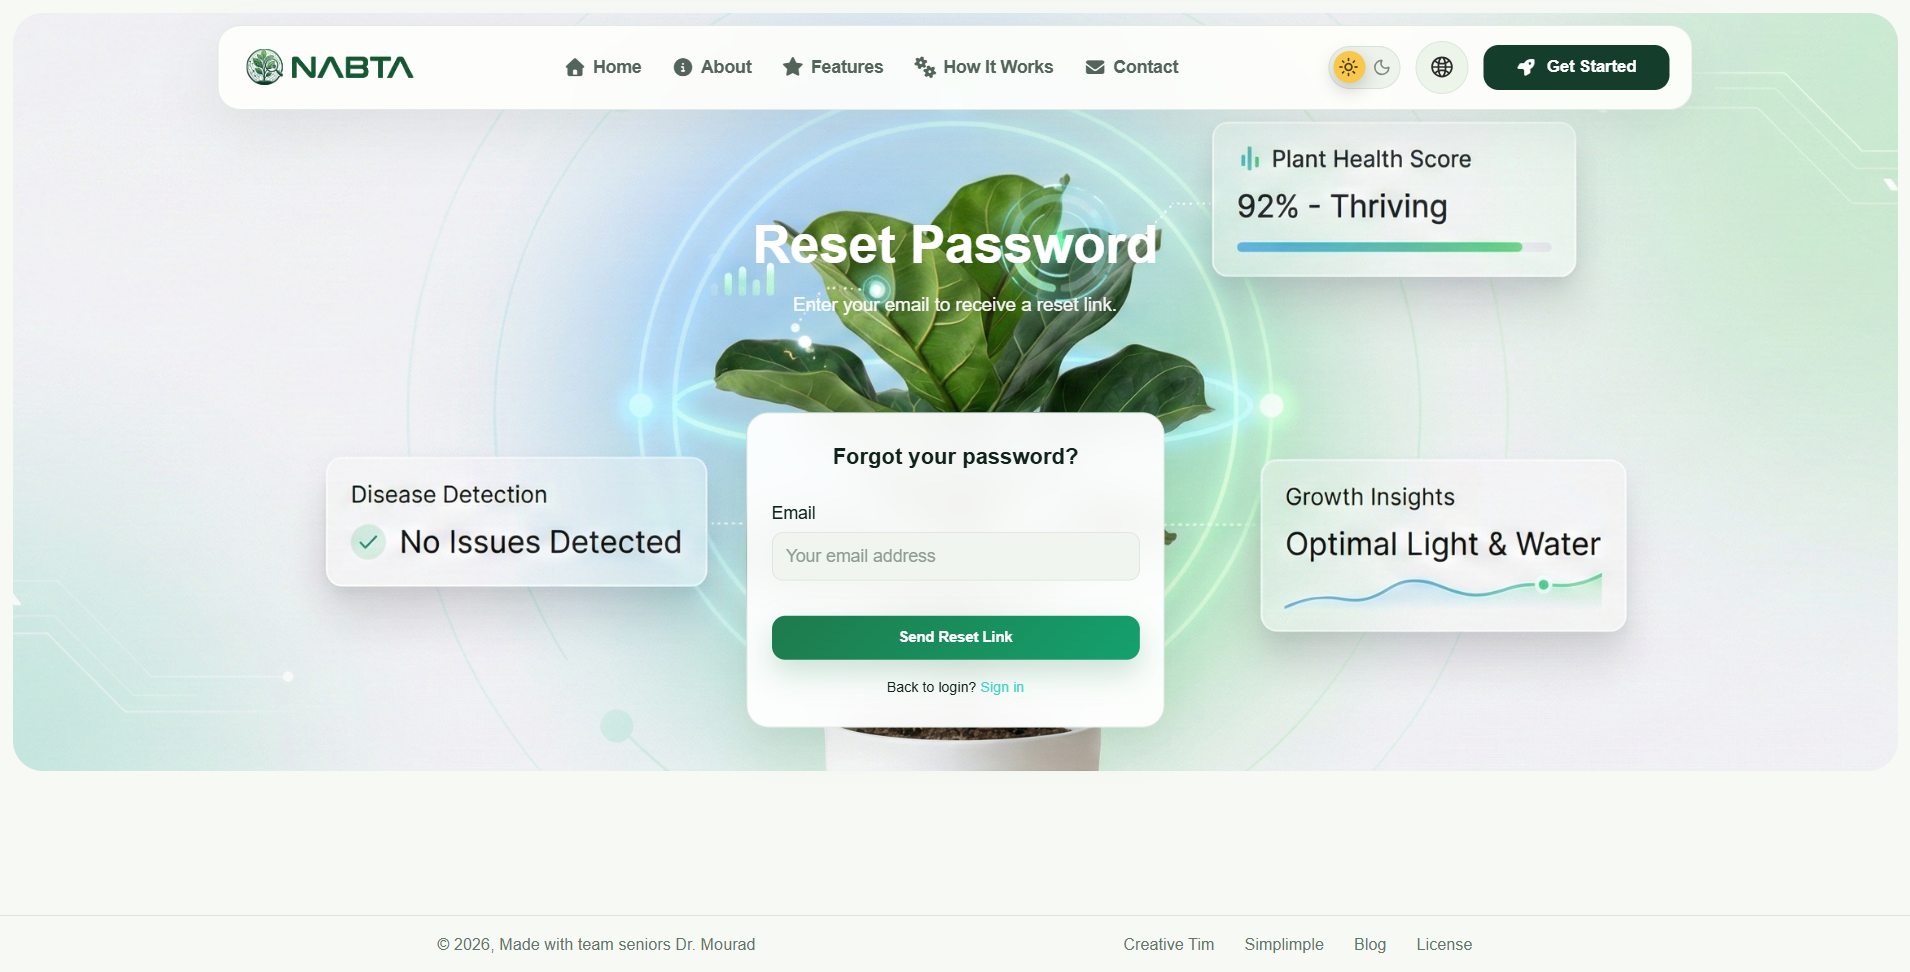
\includegraphics[width=.85\textwidth]{assets/screenshots/reset_password.png}
\caption{Password Recovery Interface}
\label{fig:reset_password}
\end{figure}

%==============================================================================
\subsection{Plant Analysis Interface}
\label{subsec:plant_analysis}

The Plant Analysis module represents the primary functionality of the NABTA platform. It enables users to upload plant leaf images for automatic disease diagnosis through the integrated artificial intelligence pipeline.

The interface supports drag-and-drop image uploading as well as conventional file selection. Before processing begins, the uploaded image is validated to ensure that only supported image formats are accepted.

Once the image is submitted, the frontend sends it asynchronously to the FastAPI backend, where the complete AI pipeline is executed.

\begin{figure}[H]
\centering
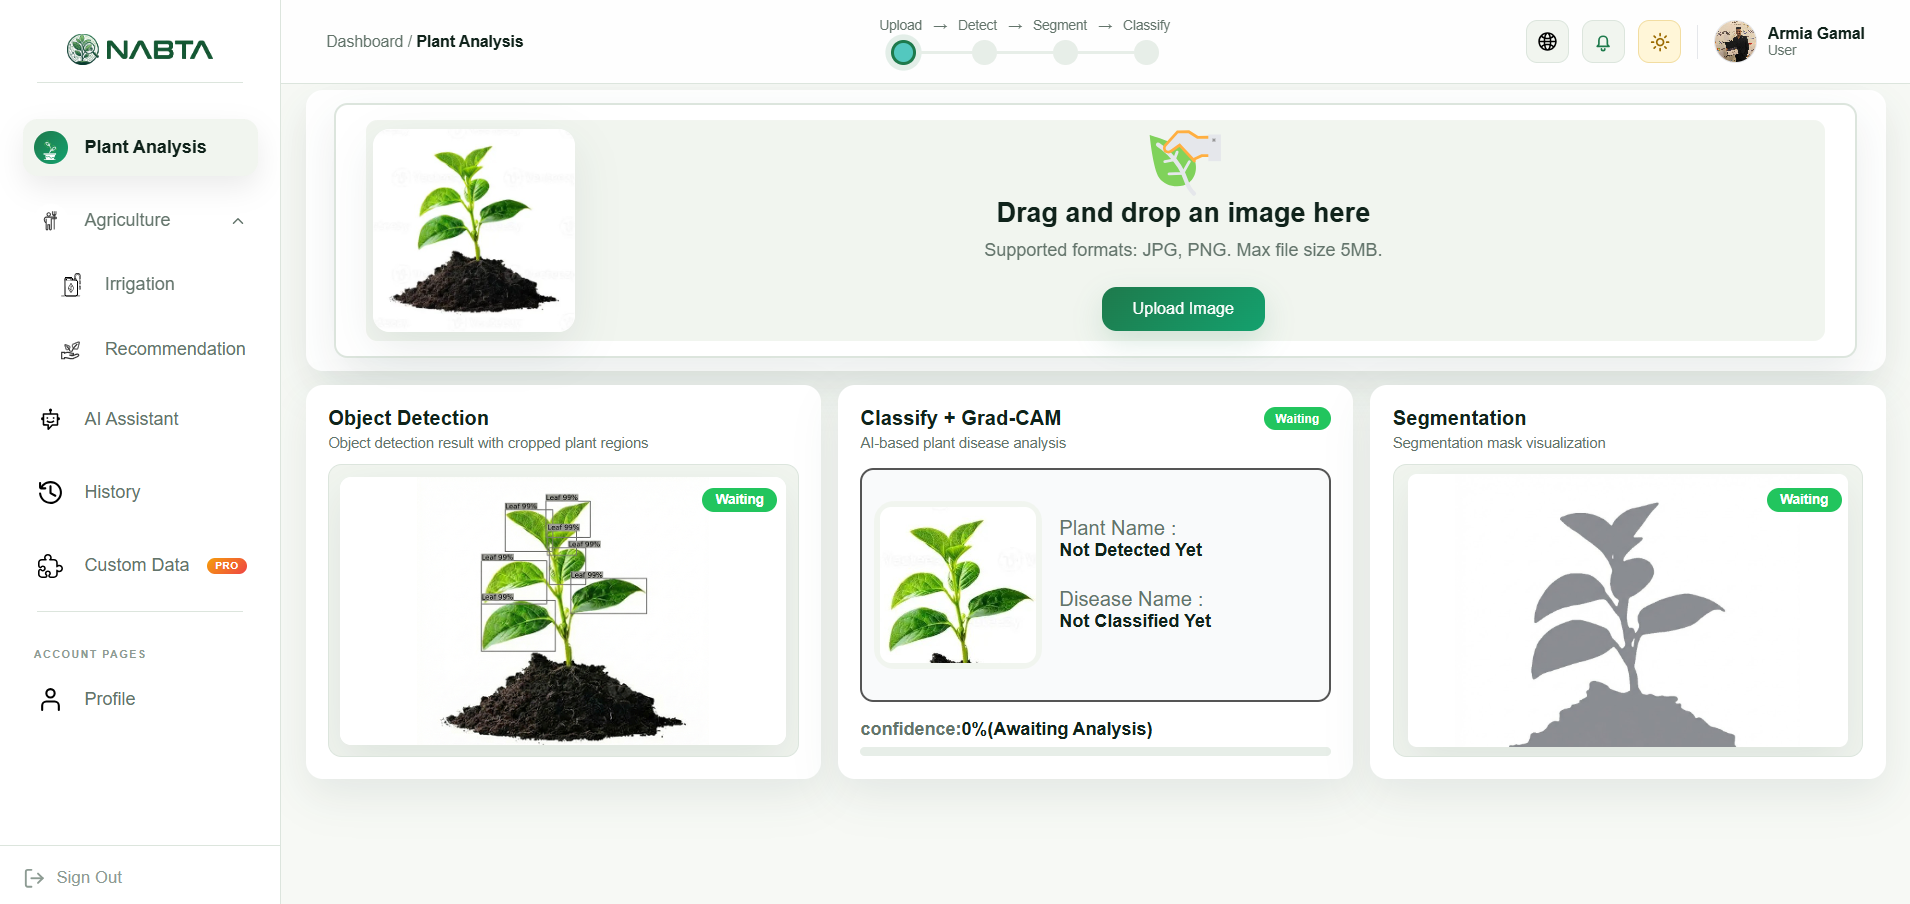
\includegraphics[width=\textwidth]{assets/screenshots/plant_analysis_upload.png}
\caption{Plant Analysis Upload Interface}
\label{fig:plant_upload}
\end{figure}

%==============================================================================
%==============================================================================
\subsection{Plant Disease Analysis Results}
\label{subsec:analysis_results}

After the uploaded image is processed, the NABTA platform presents a unified analysis interface that visualizes the complete artificial intelligence pipeline. Instead of displaying only the predicted disease, the system provides the outputs of all integrated computer vision models within a single dashboard, allowing users to understand each stage of the diagnosis process.

The interface presents:

\begin{itemize}
\item The uploaded plant image.
\item YOLOv8x object detection with the detected leaf bounding box.
\item U-Net semantic segmentation of the leaf.
\item CNN-based plant species and disease classification.
\item Prediction confidence score.
\item Disease severity estimation.
\item Direct access to the complete disease analysis report.
\end{itemize}

Displaying all analysis stages together improves transparency and enables users to verify the complete decision-making process rather than relying solely on the final prediction. This integrated visualization also demonstrates the interaction between the detection, segmentation, and classification models within the proposed NABTA pipeline.

\begin{figure}[H]
\centering
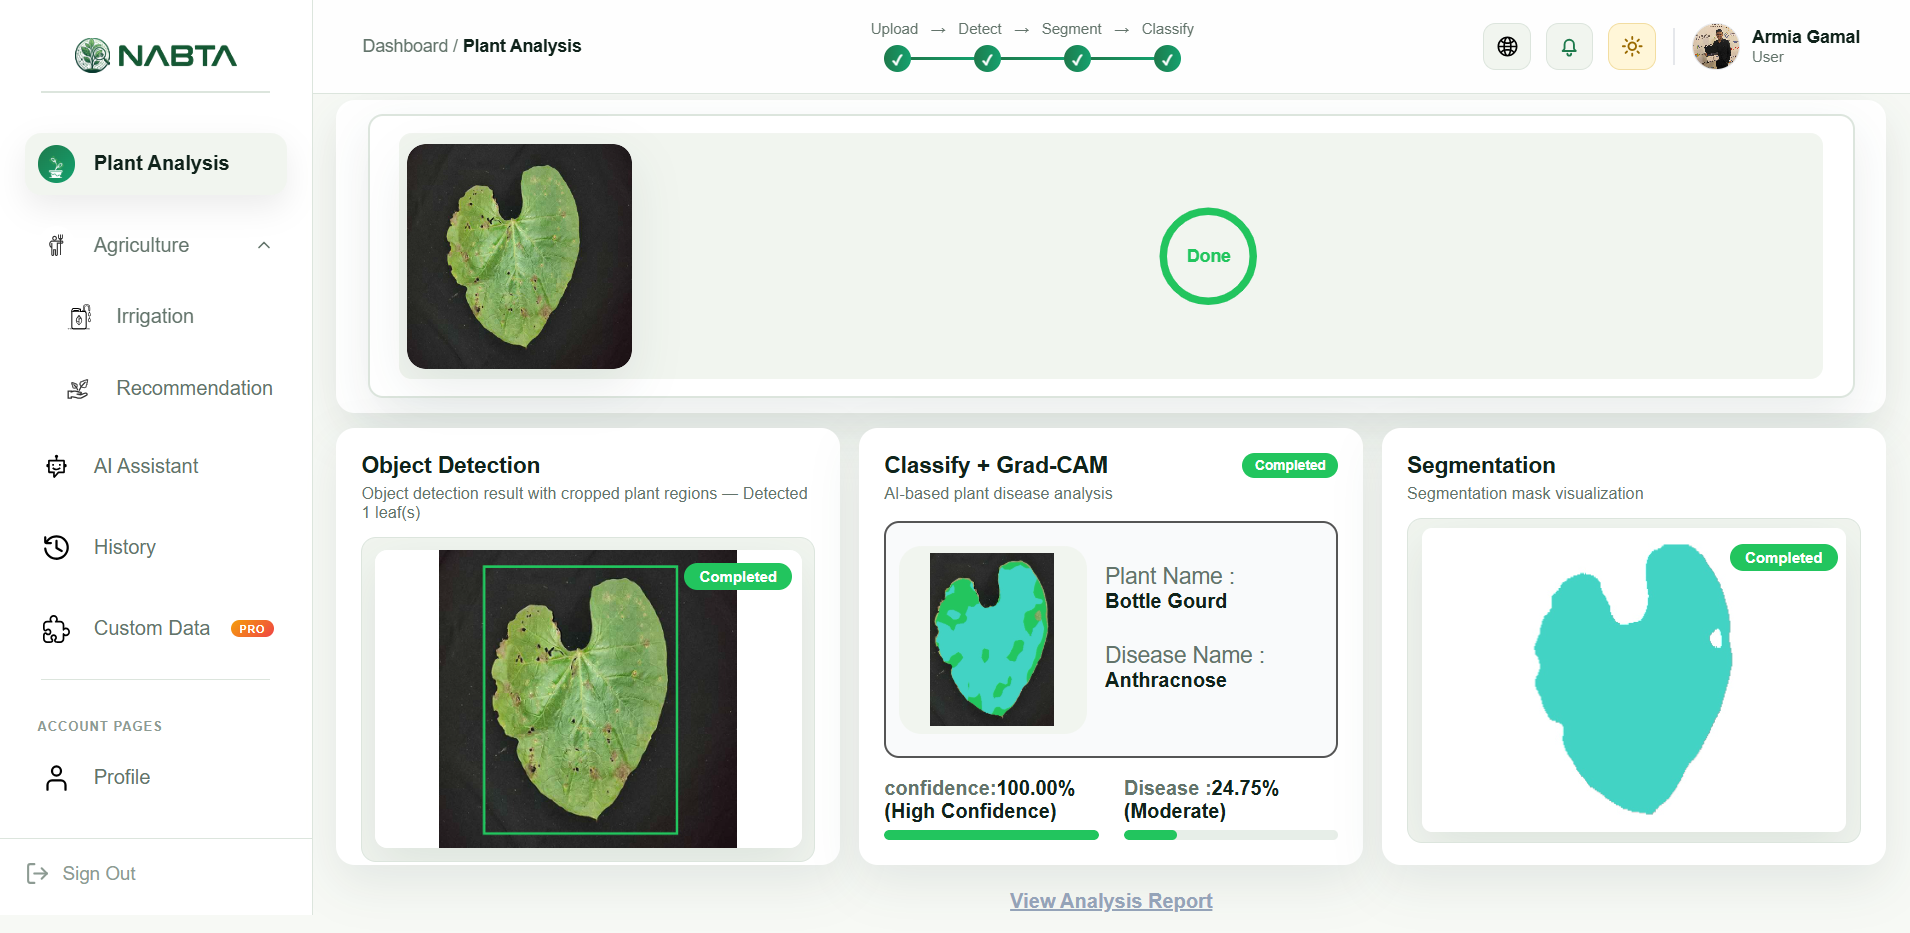
\includegraphics[width=\textwidth]{assets/screenshots/analysis_results.png}
\caption{Integrated Plant Disease Analysis Interface Showing the Outputs of YOLOv8x Detection, U-Net Segmentation, CNN Classification, Confidence Score, and Disease Severity Estimation}
\label{fig:analysis_results}
\end{figure}

%==============================================================================
\subsection{Disease Diagnosis Report}
\label{subsec:disease_report}

Following image analysis, NABTA generates a detailed disease diagnosis report summarizing all extracted information.

The report contains the predicted disease class, confidence score, detected plant species, disease severity level, Grad-CAM visualization, and recommended treatment guidelines.

This report provides users with a complete overview of the analysis outcome while serving as a basis for subsequent agricultural recommendations.

\begin{figure}[H]
\centering
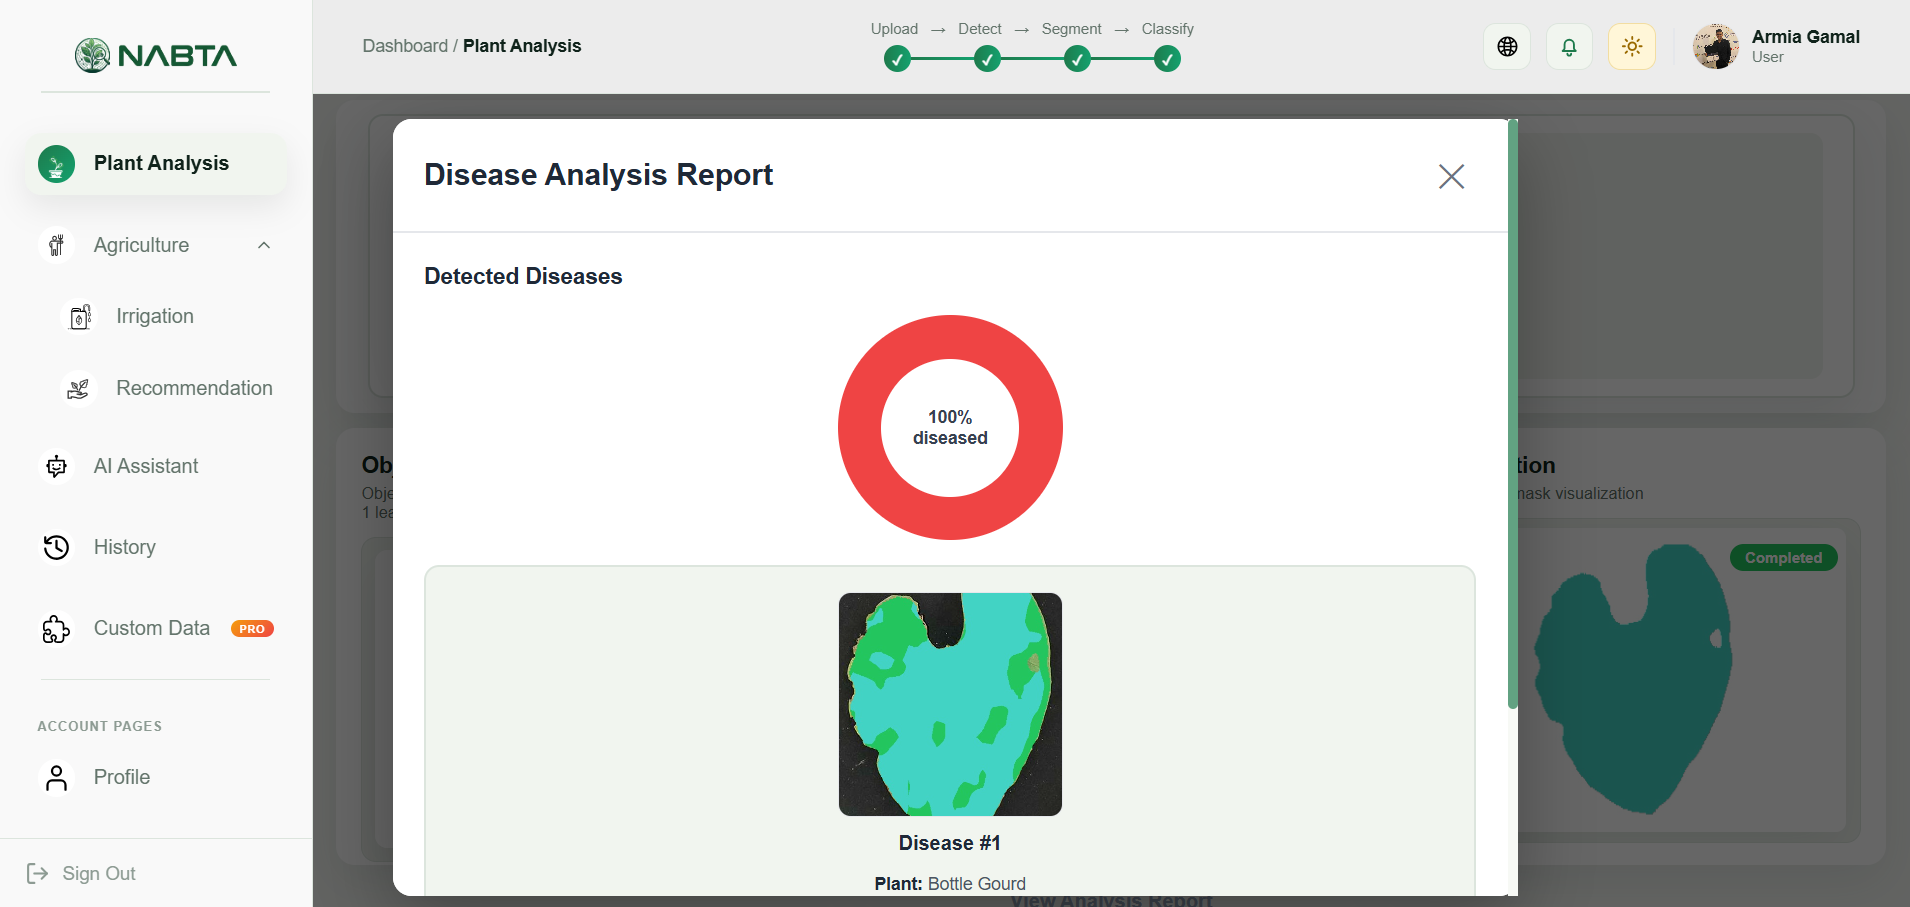
\includegraphics[width=\textwidth]{assets/screenshots/disease_report.png}
\caption{Disease Analysis Report}
\label{fig:disease_report}
\end{figure}

%==============================================================================
\subsection{AI Agricultural Assistant}
\label{subsec:assistant}

To provide intelligent agricultural consultation beyond disease diagnosis, NABTA integrates an AI-powered conversational assistant.

The assistant combines Cohere's Large Language Model with Retrieval-Augmented Generation (RAG), enabling it to retrieve domain-specific agricultural knowledge before generating responses.

Users may ask questions regarding disease symptoms, treatment methods, crop management, irrigation practices, fertilizers, and general farming recommendations.

The chatbot supports both Arabic and English, providing context-aware responses based on the retrieved agricultural knowledge base.

\begin{figure}[H]
\centering
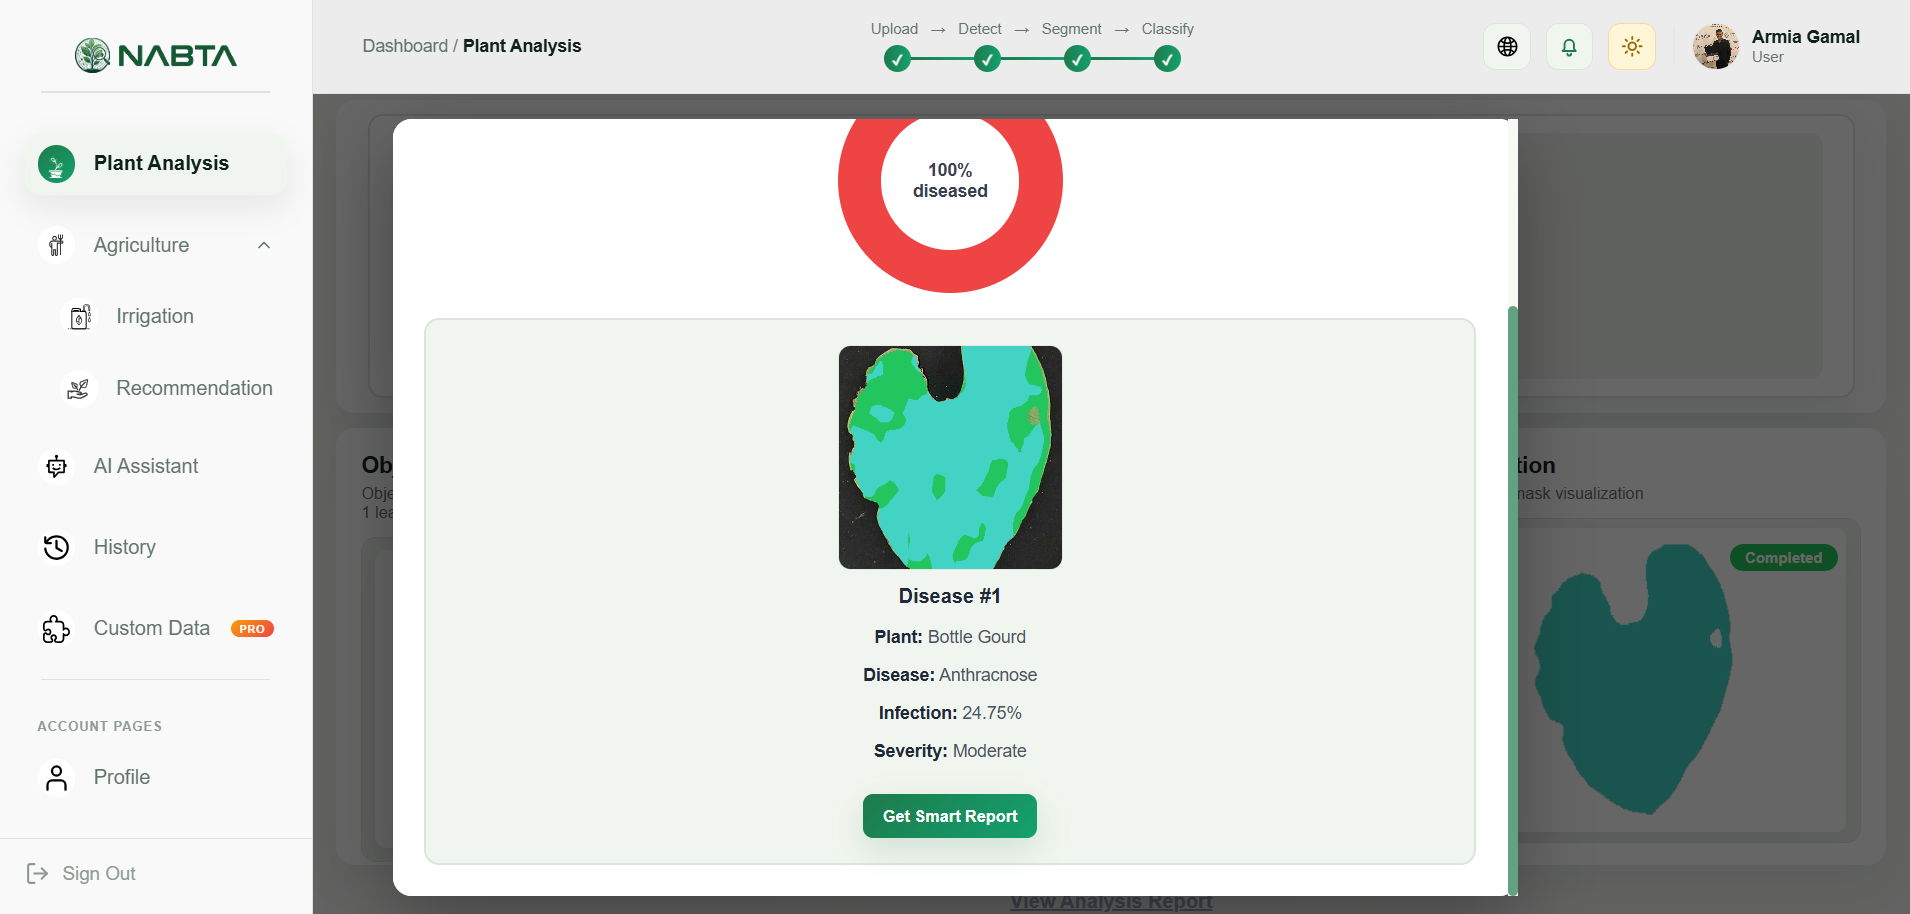
\includegraphics[width=\textwidth]{assets/screenshots/ai_assistant.png}
\caption{AI Agricultural Assistant}
\label{fig:assistant}
\end{figure}

%==============================================================================
\subsection{AI Recommendations}
\label{subsec:recommendations}

After completing the disease diagnosis process, the platform automatically generates intelligent recommendations to assist users in making informed agricultural decisions.

The recommendation engine combines the outputs of the disease classification model with the knowledge retrieved by the Retrieval-Augmented Generation (RAG) system. Based on the detected disease, the platform provides practical guidance regarding treatment methods, disease prevention strategies, suitable pesticides or fungicides, irrigation considerations, and crop management practices.

Presenting recommendations immediately after diagnosis enables users to move directly from disease identification to actionable agricultural decisions.

\begin{figure}[H]
\centering
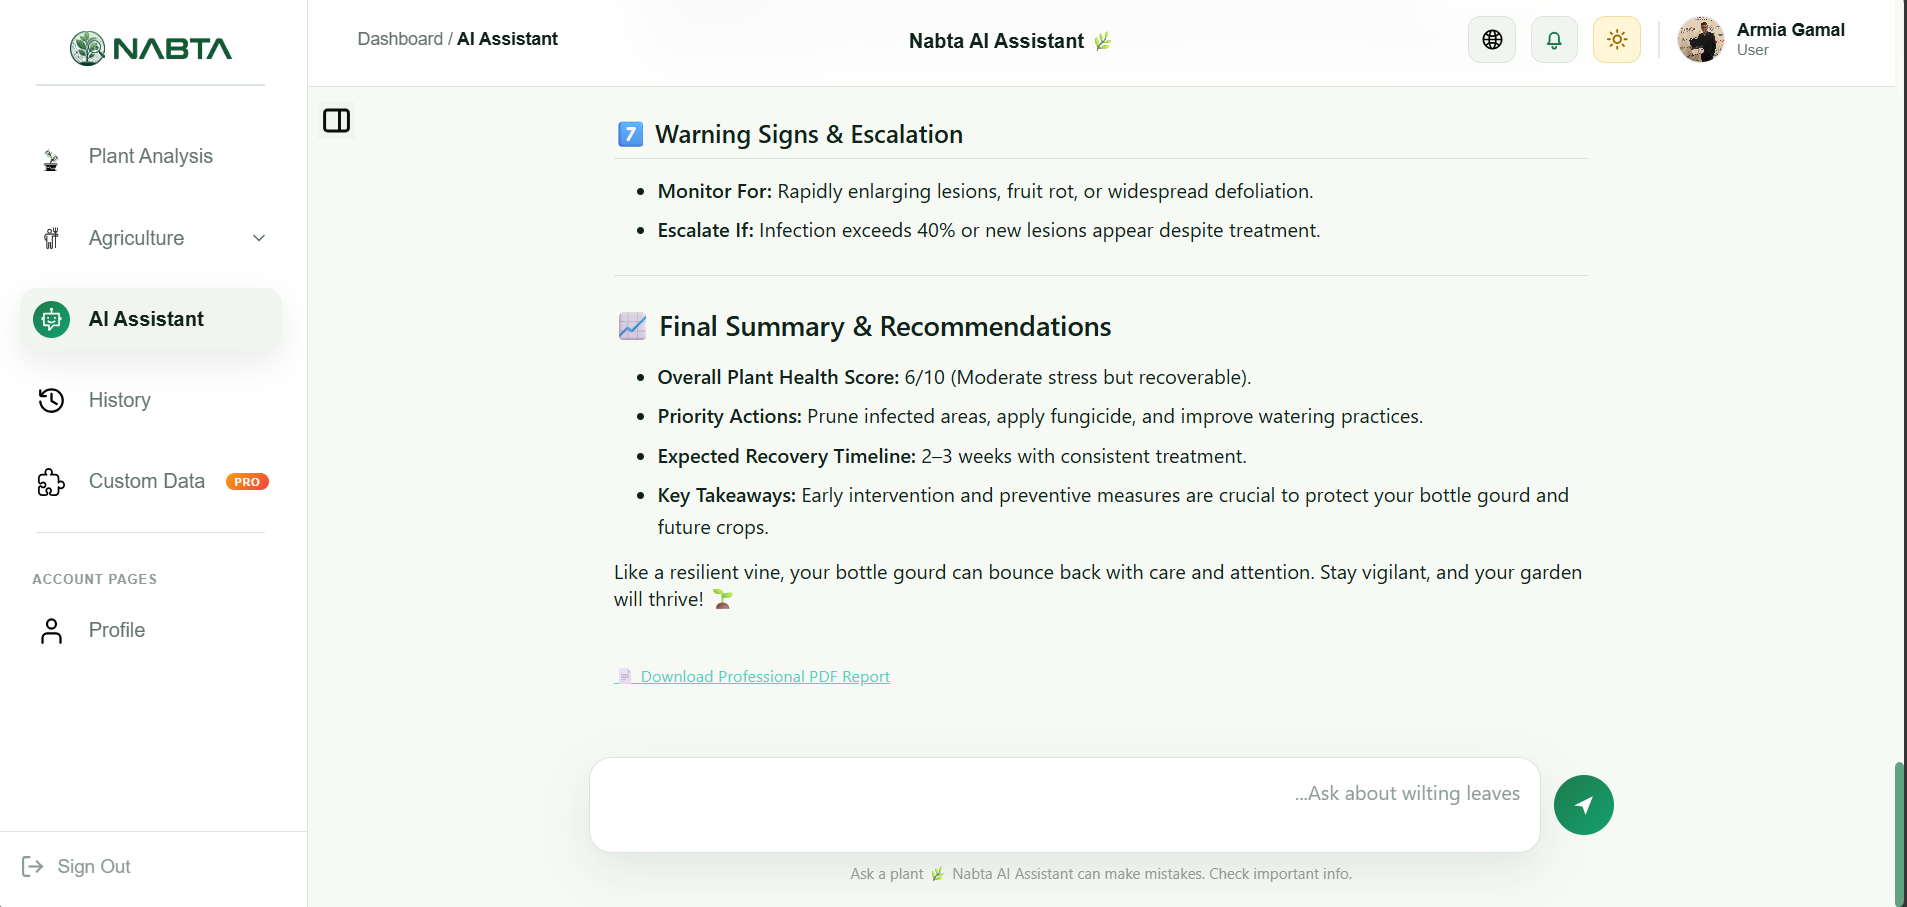
\includegraphics[width=\textwidth]{assets/screenshots/ai_recommendations.png}
\caption{AI-Based Agricultural Recommendations}
\label{fig:recommendations}
\end{figure}

%==============================================================================
\subsection{PDF Disease Report}
\label{subsec:pdf_report}

To facilitate documentation and information sharing, NABTA automatically generates a downloadable PDF report for every completed disease analysis.

The generated report summarizes all information produced during the AI pipeline, including the uploaded image, detected disease, confidence score, Grad-CAM visualization, disease severity, recommended treatment, and additional agricultural guidance.

The PDF report enables farmers, agricultural engineers, and researchers to archive diagnosis results or share them with specialists for further consultation.

\begin{figure}[H]
\centering
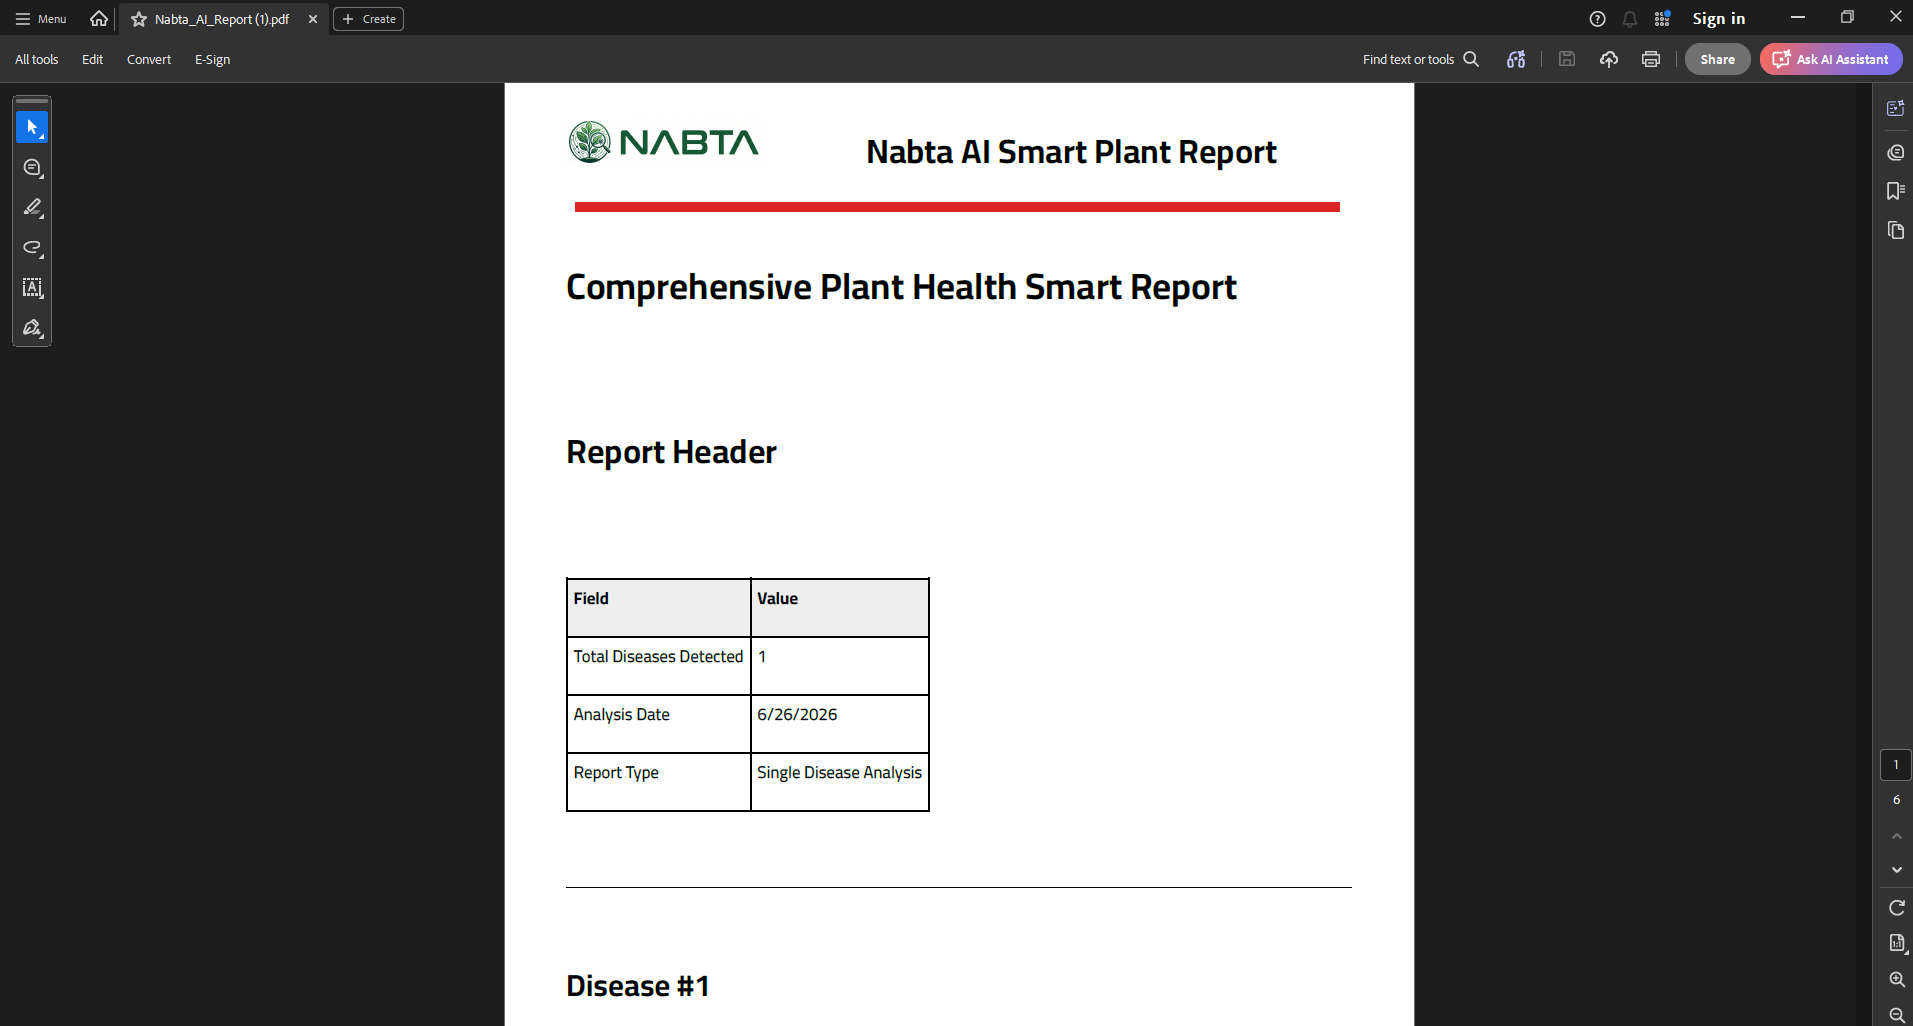
\includegraphics[width=\textwidth]{assets/screenshots/pdf_report.png}
\caption{Automatically Generated PDF Disease Report}
\label{fig:pdf_report}
\end{figure}

%==============================================================================
\subsection{Analysis Dashboard}
\label{subsec:dashboard}

The dashboard provides users with an integrated overview of their activities and the overall performance of the NABTA platform.

It summarizes important information including the total number of analyses, diagnosed diseases, healthy plant detections, generated reports, and recent AI activities. Interactive widgets and graphical indicators allow users to quickly monitor system usage and recent analysis results.

The dashboard serves as the central navigation point after user authentication.

\begin{figure}[H]
\centering
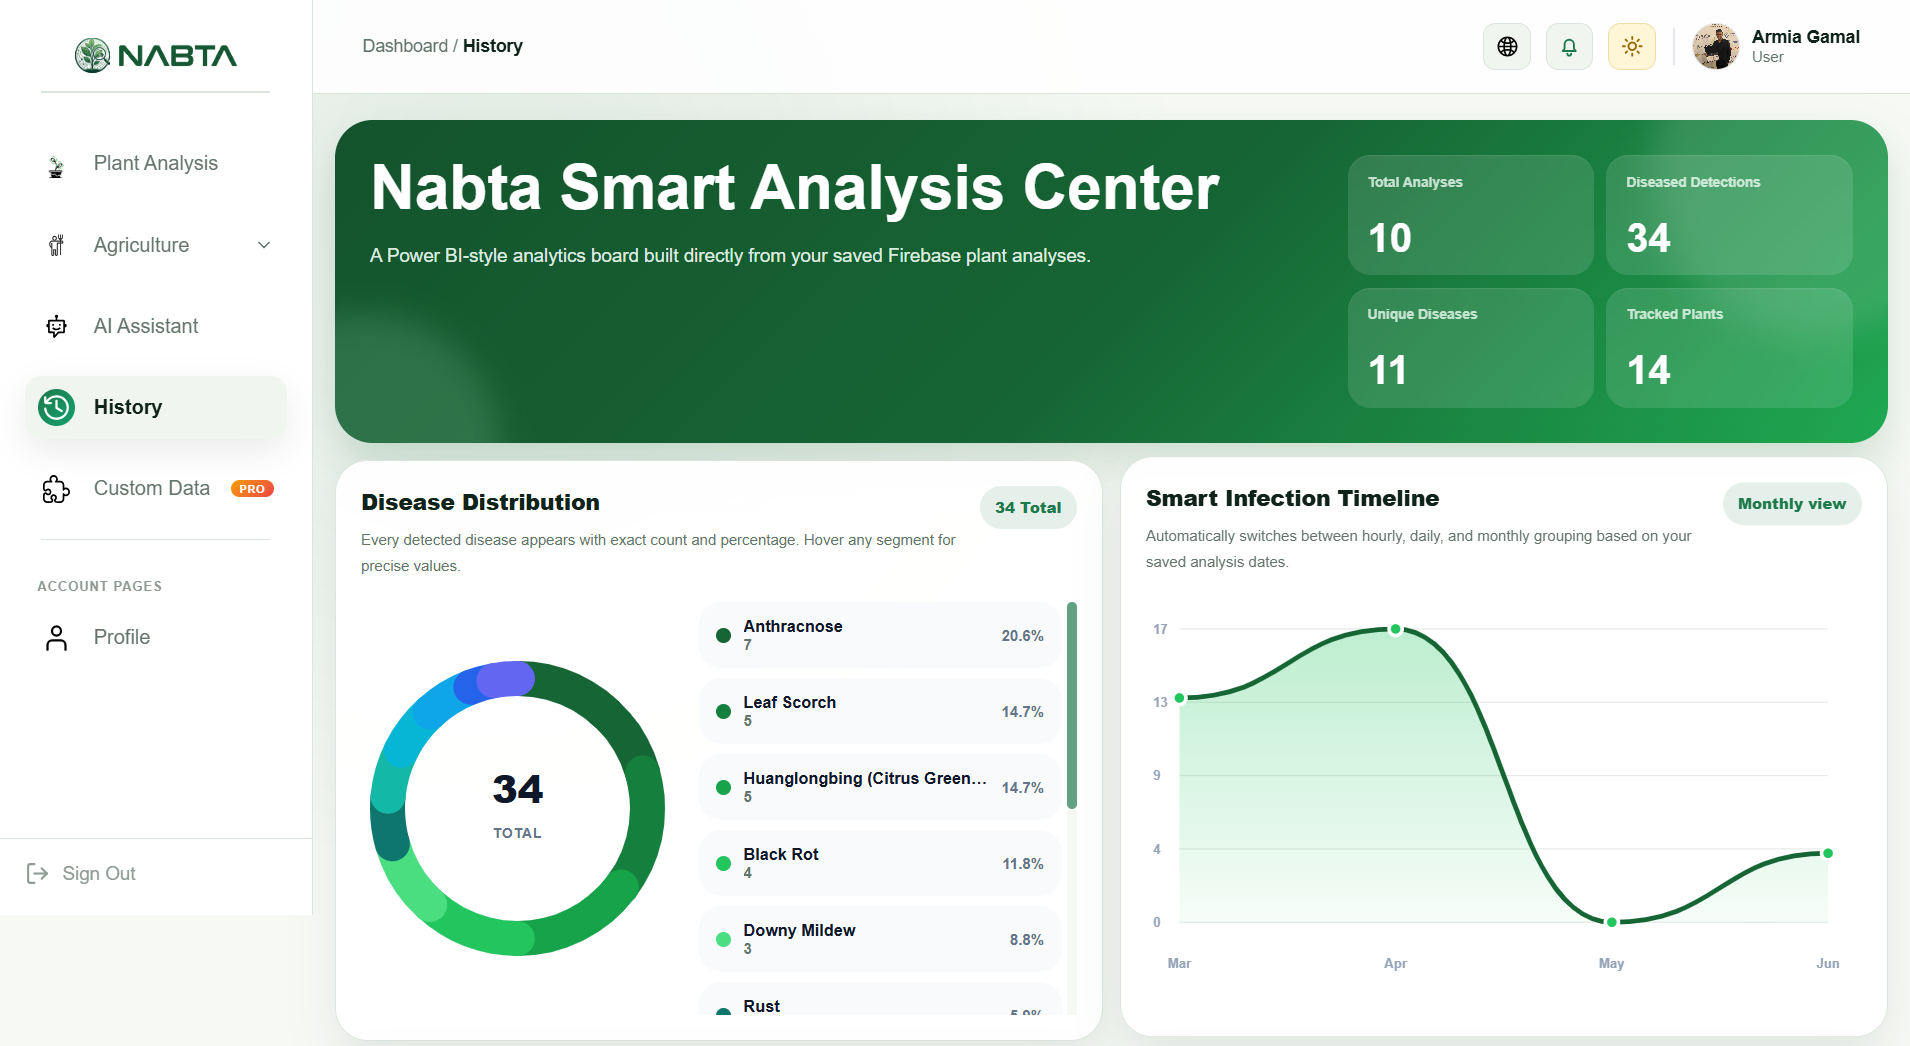
\includegraphics[width=\textwidth]{assets/screenshots/dashboard.png}
\caption{Analysis Dashboard}
\label{fig:dashboard}
\end{figure}

%==============================================================================
\subsection{Plant and Disease Analytics}
\label{subsec:analytics}

NABTA includes an analytics module that visualizes historical disease statistics and plant health trends.

Interactive charts display the distribution of detected diseases, healthy versus diseased samples, frequently analyzed plant species, confidence score distributions, and temporal analysis trends.

These visualizations assist users in understanding disease prevalence while providing useful insights for monitoring crop health over time.

\begin{figure}[H]
\centering
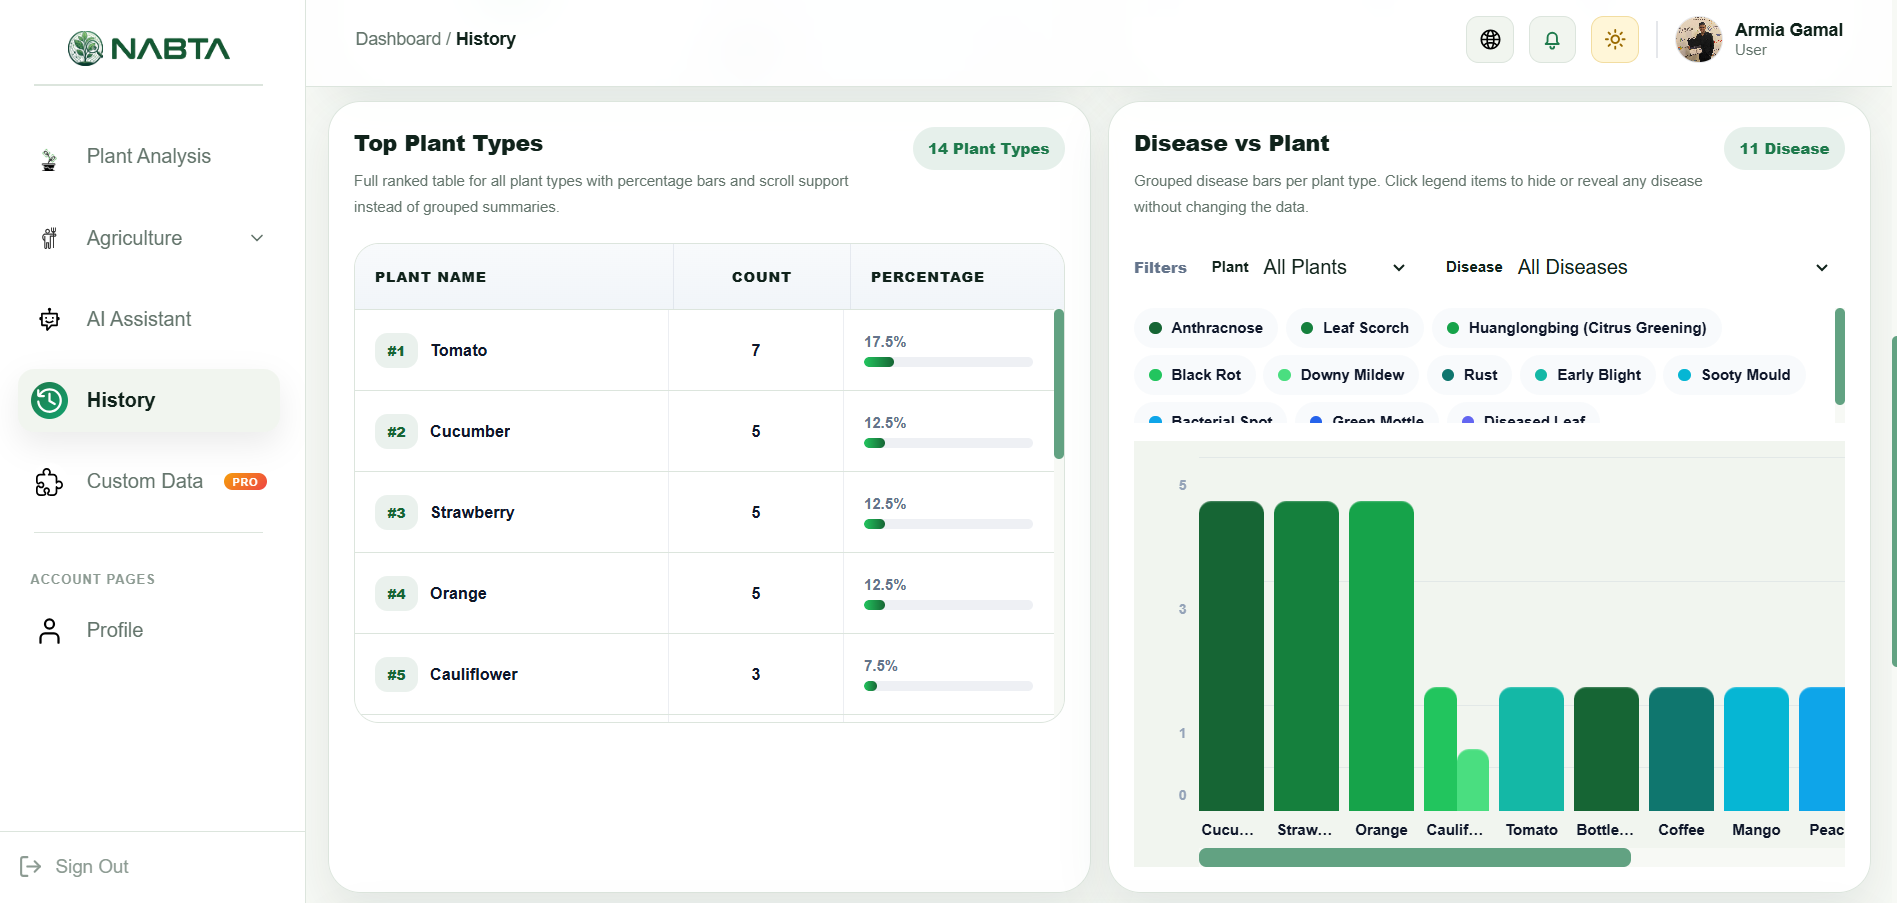
\includegraphics[width=\textwidth]{assets/screenshots/analytics.png}
\caption{Plant and Disease Analytics Dashboard}
\label{fig:analytics}
\end{figure}

%==============================================================================
\subsection{Analysis History}
\label{subsec:history}

Every completed analysis is securely stored within the user's account, allowing previous diagnoses to be reviewed at any time.

The history interface displays previously analyzed images together with their corresponding disease predictions, confidence scores, timestamps, and generated reports.

Users can search, filter, revisit, or download previous analysis reports without repeating the disease detection process.

Maintaining historical records improves traceability and enables long-term monitoring of crop health.

\begin{figure}[H]
\centering
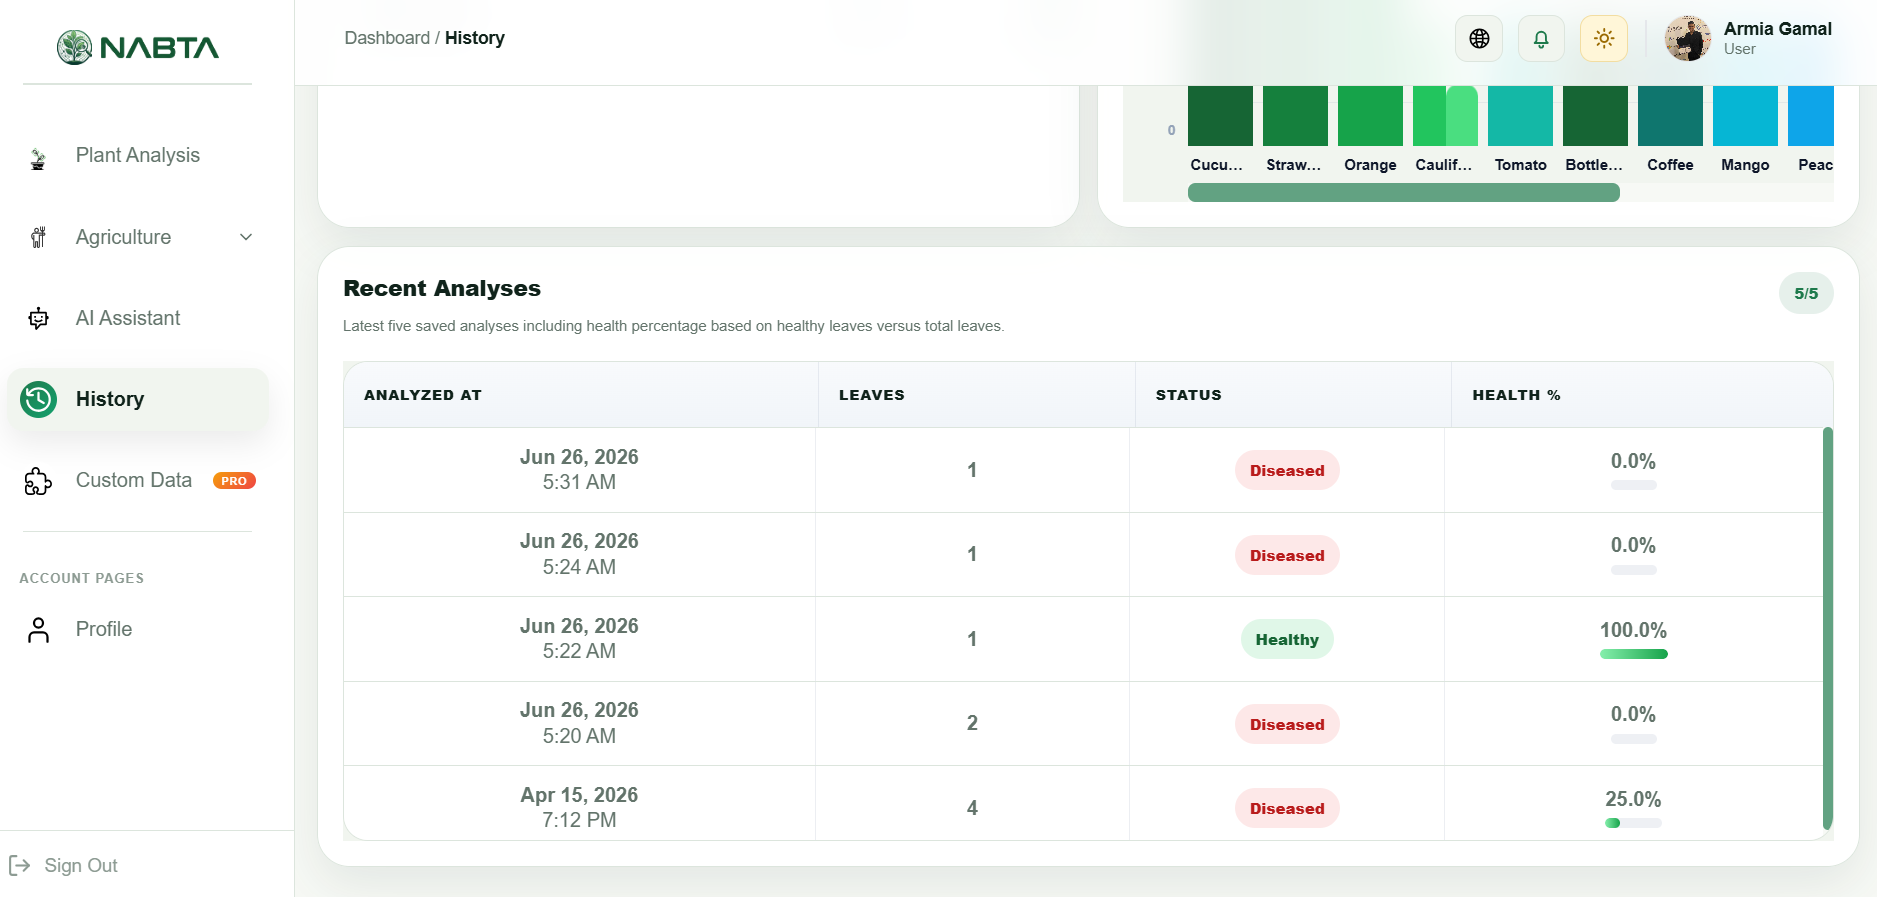
\includegraphics[width=\textwidth]{assets/screenshots/history.png}
\caption{Analysis History Interface}
\label{fig:history}
\end{figure}

%==============================================================================
\subsection{Irrigation Management}
\label{subsec:irrigation}

The irrigation management module assists farmers in making informed irrigation decisions using machine learning models trained on agricultural and environmental data.

Users provide soil moisture, soil type, crop type, temperature, humidity, rainfall, and other environmental parameters. The platform then predicts whether irrigation is required and estimates the expected crop water requirement.

The interface presents the prediction results in a clear and user-friendly format, enabling farmers to optimize irrigation schedules while reducing unnecessary water consumption.

\begin{figure}[H]
\centering
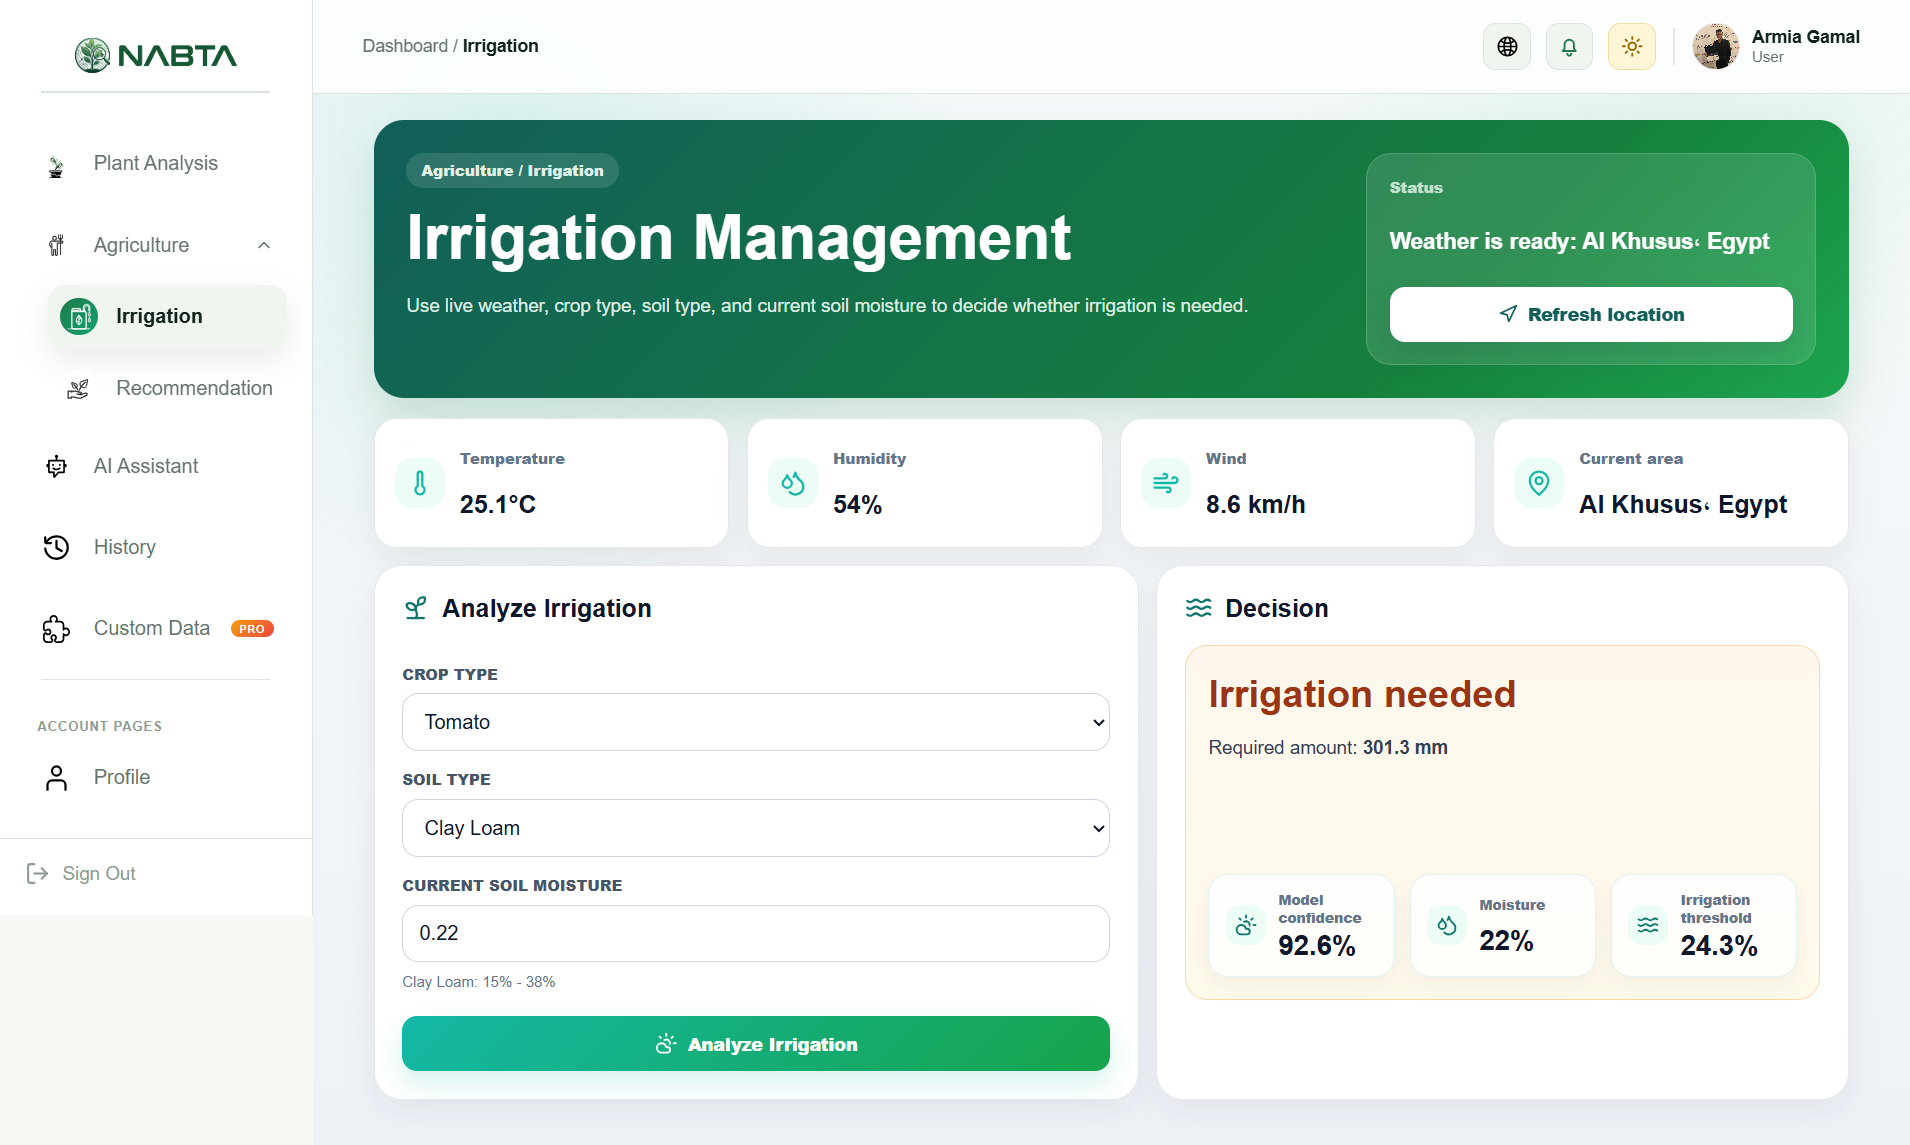
\includegraphics[width=\textwidth]{assets/screenshots/irrigation_management.png}
\caption{Smart Irrigation Management Interface}
\label{fig:irrigation}
\end{figure}

%==============================================================================
\subsection{Crop Recommendation}
\label{subsec:crop}

The crop recommendation module suggests the most suitable crop based on soil properties and environmental conditions.

Users enter the available Nitrogen (N), Phosphorus (P), Potassium (K), soil type, pH, temperature, humidity, and rainfall values. These inputs are processed by a Random Forest classifier trained on a regenerated agricultural dataset incorporating crop--soil suitability knowledge.

The system predicts the most appropriate crop together with confidence scores, allowing users to select crops that best match the current environmental conditions.

\begin{figure}[H]
\centering
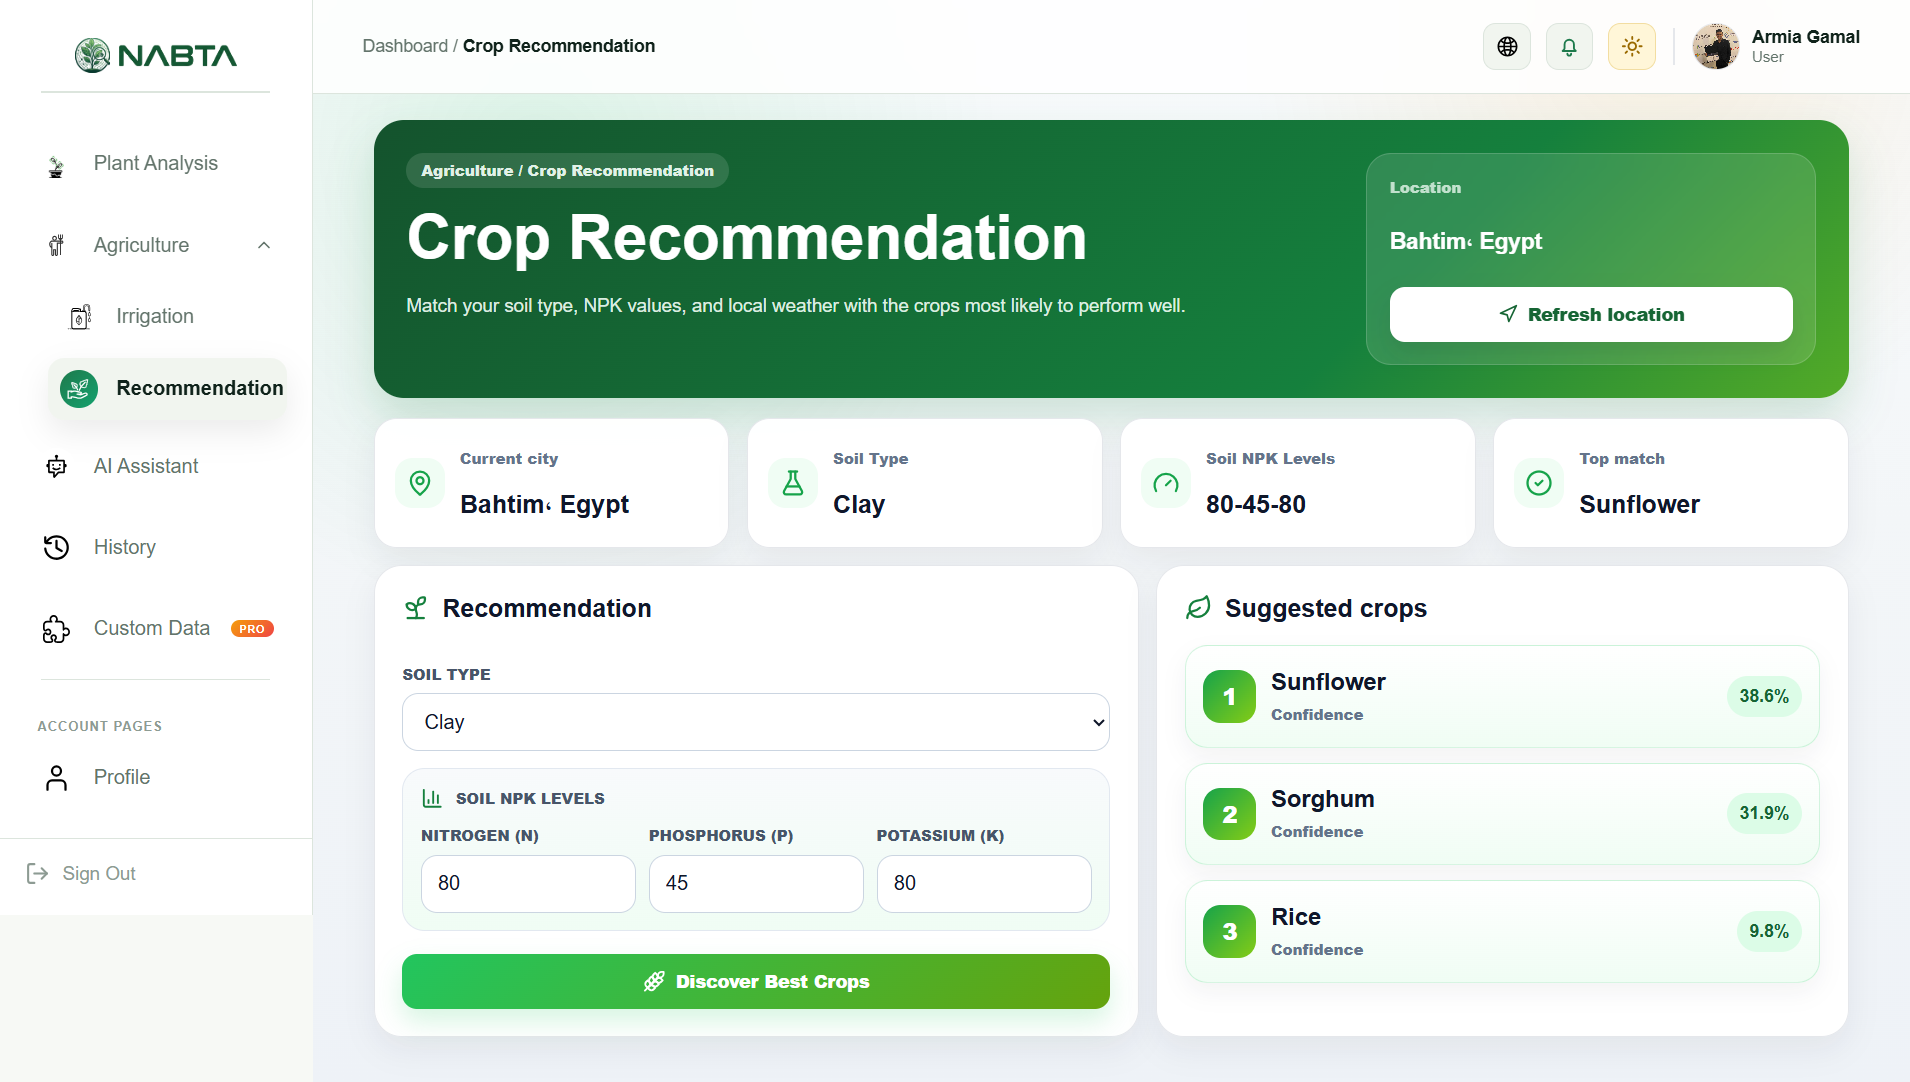
\includegraphics[width=\textwidth]{assets/screenshots/crop_recommendation.png}
\caption{Crop Recommendation Interface}
\label{fig:crop}
\end{figure}

%==============================================================================
\subsection{Custom Data Management}
\label{subsec:custom_data}

The platform includes a custom data management module that allows administrators to manage agricultural knowledge and user-generated data.

Authorized users can create, update, delete, and organize custom records through an intuitive interface. This functionality enables continuous expansion of the agricultural knowledge base while maintaining data consistency across the platform.

The management interface simplifies dataset maintenance without requiring direct database access.

\begin{figure}[H]
\centering
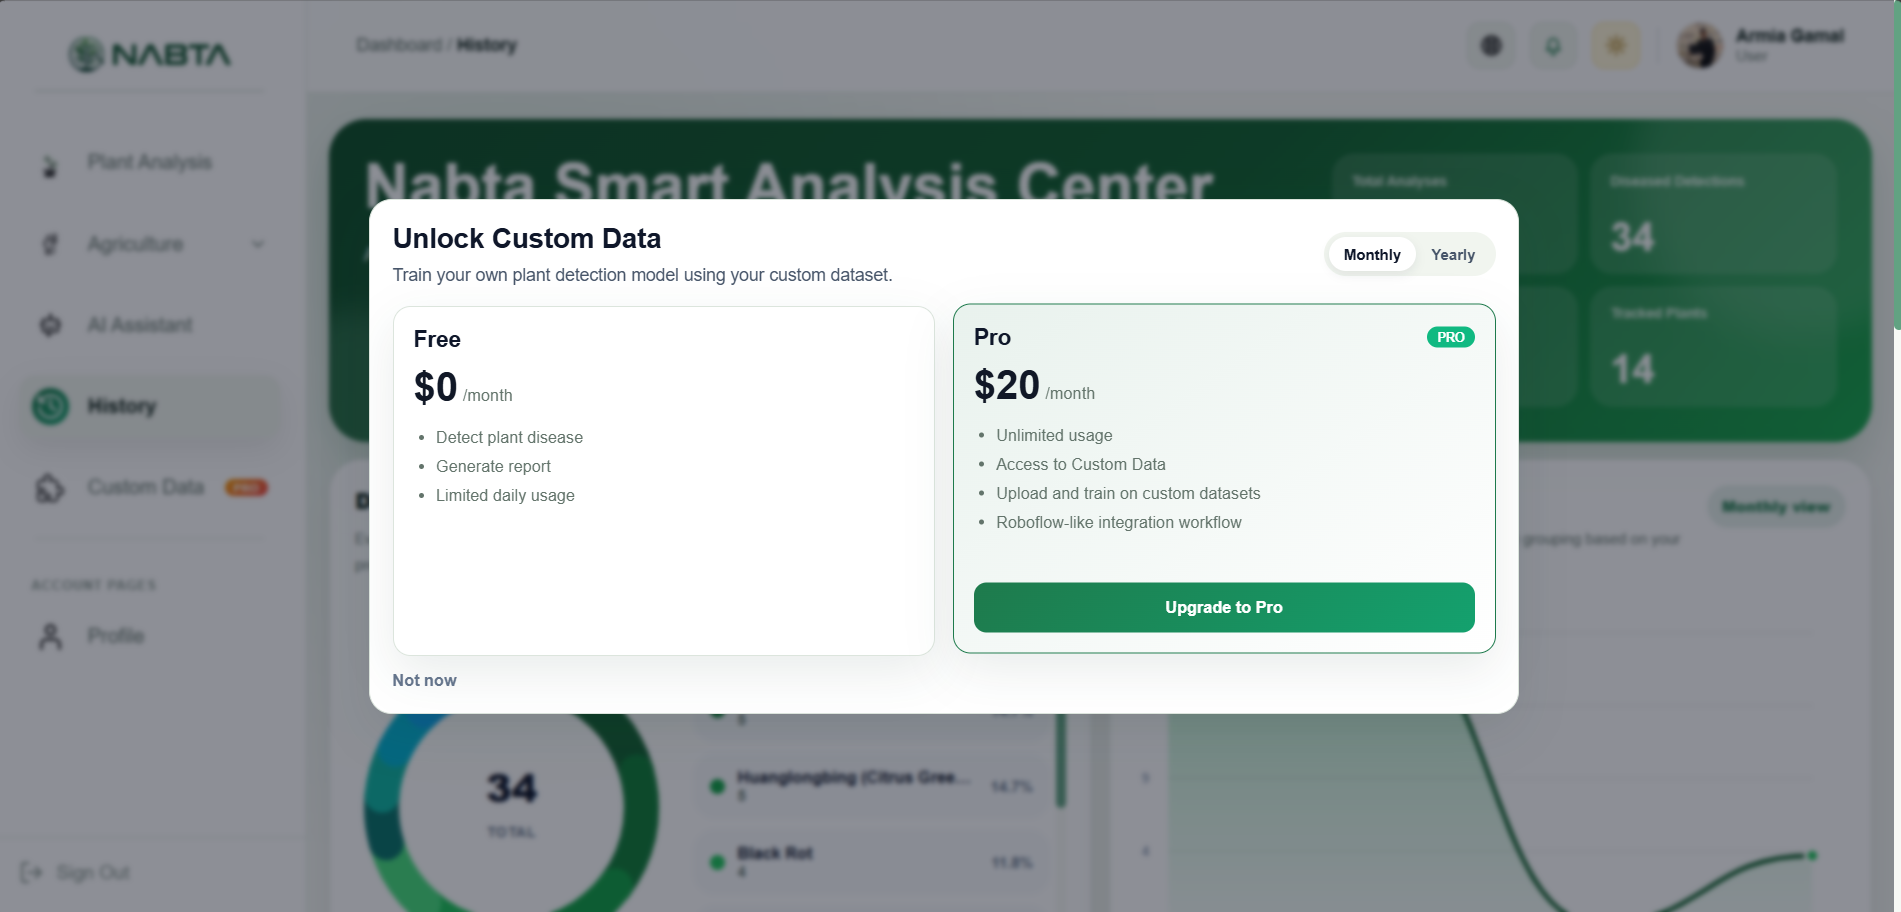
\includegraphics[width=\textwidth]{assets/screenshots/custom_data_management.png}
\caption{Custom Data Management Interface}
\label{fig:custom_data}
\end{figure}

%==============================================================================
\subsection{User Profile}
\label{subsec:profile}

Each registered user has a personalized profile containing account information, analysis statistics, generated reports, and personal preferences.

The profile page allows users to update personal information, change passwords, manage profile settings, and review their overall activity within the platform.

This centralized profile improves personalization while providing quick access to frequently used services.

\begin{figure}[H]
\centering
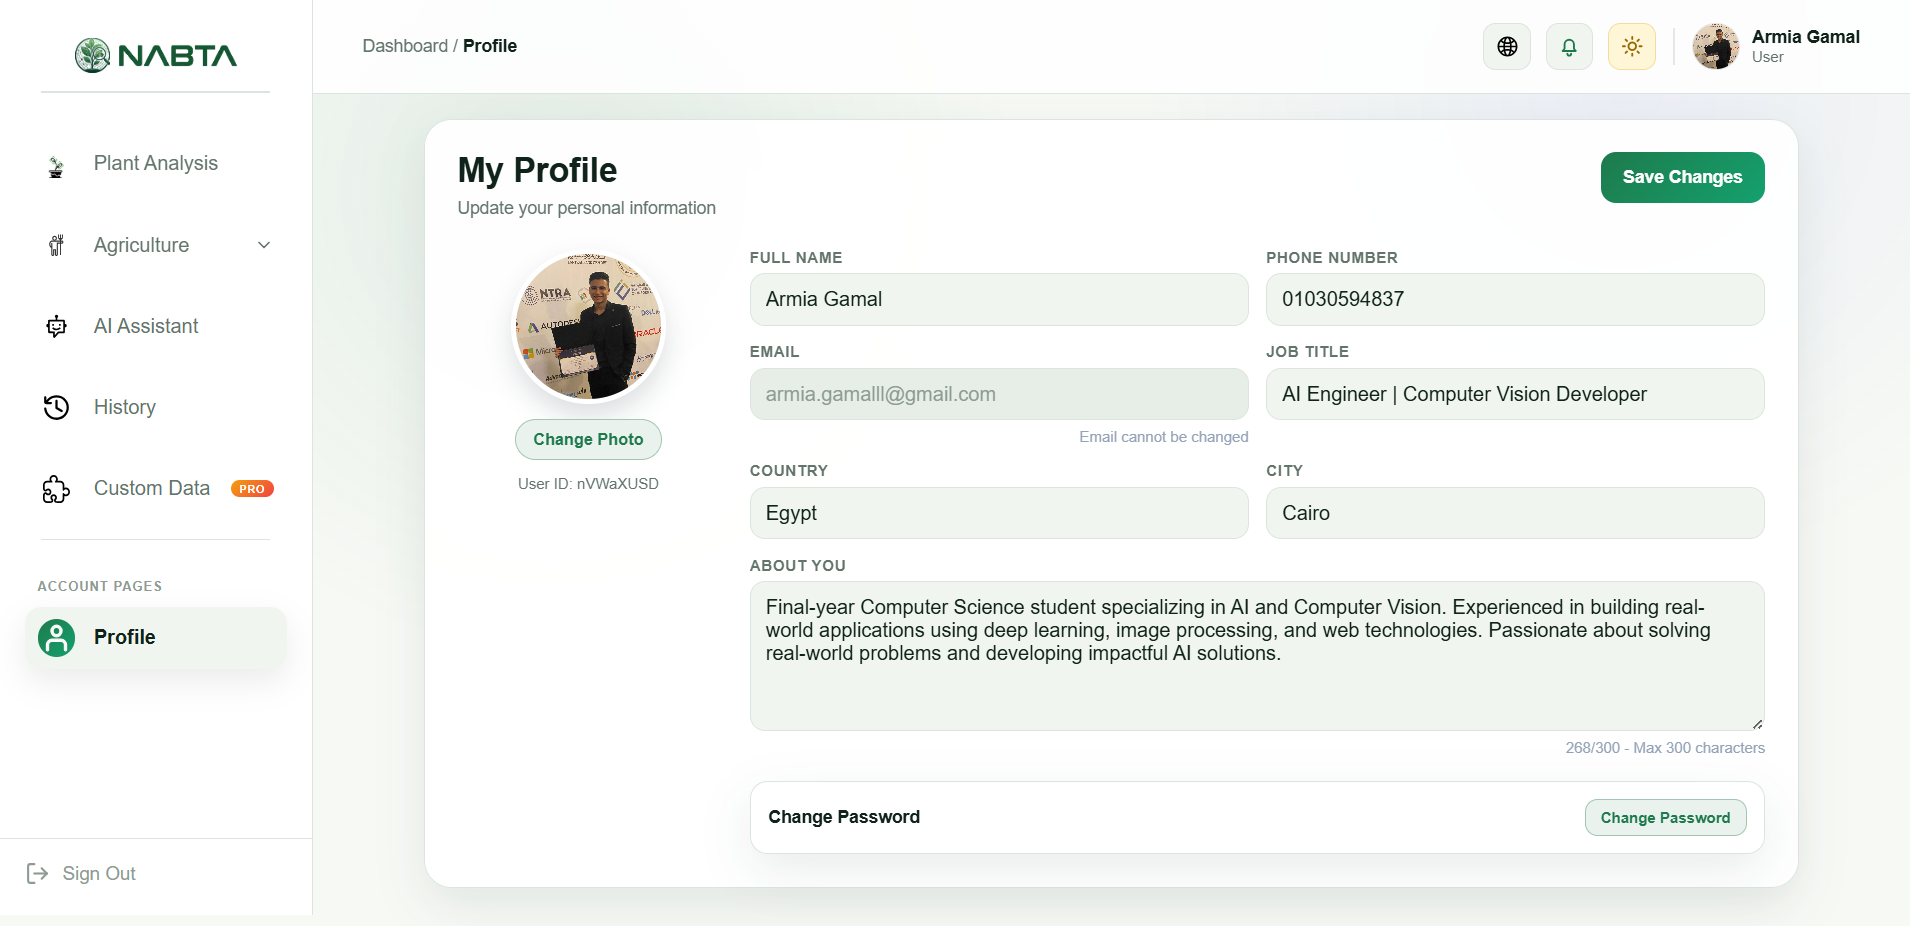
\includegraphics[width=\textwidth]{assets/screenshots/user_profile.png}
\caption{User Profile Interface}
\label{fig:profile}
\end{figure}

%==============================================================================
\section{Backend Implementation}
\label{sec:backend}

The backend of NABTA was implemented using FastAPI, providing a lightweight and high-performance RESTful API architecture.

FastAPI coordinates communication between the frontend, artificial intelligence models, Firebase services, and external APIs. The backend is responsible for image processing, model inference, authentication, report generation, chatbot interaction, and database communication.

Asynchronous request handling enables multiple users to access AI services simultaneously while maintaining low response latency.

%==============================================================================
\section{Artificial Intelligence Integration}
\label{sec:ai_integration}

One of the primary objectives of NABTA is the seamless integration of multiple artificial intelligence models within a single production-ready platform.

The AI pipeline consists of:

\begin{itemize}
\item YOLOv8x for infected leaf detection.
\item U-Net with EfficientNet-B0 encoder for semantic segmentation.
\item Custom CNN for disease classification.
\item Grad-CAM for explainability and disease severity estimation.
\item Random Forest classifier for crop recommendation.
\item Random Forest classifier for irrigation decision prediction.
\item Random Forest regressor for crop water requirement estimation.
\item Cohere Large Language Model integrated with Retrieval-Augmented Generation for intelligent agricultural consultation.
\end{itemize}

All models communicate through standardized FastAPI endpoints, enabling independent deployment while maintaining seamless integration across the entire platform.

%==============================================================================
\section{Cloud Services Integration}
\label{sec:firebase}

Firebase provides the cloud infrastructure supporting authentication, secure data storage, and backend services.

The platform utilizes Firebase Authentication for secure user management, Cloud Firestore for storing analysis history and user information, and Cloud Functions for backend automation, email notifications, and secure API operations.

These cloud services improve scalability, reliability, and security while minimizing infrastructure management overhead.

%==============================================================================
\section{Chapter Summary}
\label{sec:chapter4_summary}

This chapter presented the implementation of the NABTA smart agriculture platform, including the frontend interfaces, backend services, artificial intelligence integration, and cloud infrastructure.

The implementation demonstrates how multiple AI technologies were successfully combined into a unified web-based application that supports plant disease diagnosis, crop recommendation, irrigation management, explainable artificial intelligence, PDF report generation, and intelligent agricultural consultation.

The following chapter presents the experimental evaluation and performance analysis of all implemented artificial intelligence models.

%==============================================================================
% CHAPTER 7 --- RESULTS AND EVALUATION
%==============================================================================

\chapter{Results and Evaluation}
\label{chap:results}

\chapterquote{Without data, you're just another person with an opinion.}{W. Edwards Deming}

%==============================================================================
\section{Overview}
\label{sec:results_overview}

This chapter presents the experimental evaluation of the proposed NABTA platform. The performance of each artificial intelligence component is evaluated individually, including the CNN classification model, YOLOv8 object detection model, U-Net segmentation model, Crop Recommendation model, and Smart Irrigation models. The reported results demonstrate the effectiveness of the proposed platform across all intelligent services.

All reported results are obtained using held-out test datasets that were completely separated from the training and validation datasets to ensure an unbiased evaluation of model performance.

%==============================================================================
\section{Classification Model Performance}
\label{sec:cnn_results}

\subsection{Overall Performance}
\label{subsec:cnn_acc}

The CNN classification model was evaluated on an independent test set consisting of \textbf{12,198} images covering \textbf{102} healthy and diseased plant classes collected from multiple public datasets. The model achieved an overall classification accuracy of \textbf{95.0\%}, demonstrating strong generalization across different crops, disease categories, and real-world imaging conditions.

Table~\ref{tab:cnn_metrics} summarizes the aggregate classification performance.

\begin{table}[H]
\centering
\caption{CNN Classification Model -- Overall Test Performance}
\label{tab:cnn_metrics}
\renewcommand{\arraystretch}{1.4}
\begin{tabular}{lc}
\toprule
\textbf{Metric} & \textbf{Value} \\
\midrule
Test Images & 12,198 \\
Number of Classes & 102 \\
Overall Accuracy & 95.0\% \\
Macro Precision & 95.0\% \\
Macro Recall & 94.0\% \\
Macro F1-score & 94.0\% \\
Weighted Precision & 95.0\% \\
Weighted Recall & 95.0\% \\
Weighted F1-score & 95.0\% \\
\bottomrule
\end{tabular}
\end{table}

The high weighted metrics indicate that the model performs consistently across the entire dataset, while the macro-average scores demonstrate balanced performance among the individual disease classes despite differences in class distributions.

%==============================================================================
\subsection{Representative Per-Class Performance}
\label{subsec:cnn_per_class}

Table~\ref{tab:cnn_per_class} presents representative classification results for selected plant diseases extracted from the complete classification report.

\begin{table}[H]
\centering
\caption{Representative CNN Classification Results}
\label{tab:cnn_per_class}
\renewcommand{\arraystretch}{1.4}
\begin{tabularx}{\textwidth}{X l c c c}
\toprule
\textbf{Class} &
\textbf{Plant} &
\textbf{Precision} &
\textbf{Recall} &
\textbf{F1-score} \\
\midrule

Apple Scab &
Apple &
1.00 &
1.00 &
1.00 \\

Apple Black Rot &
Apple &
1.00 &
1.00 &
1.00 \\

Apple Healthy &
Apple &
0.99 &
1.00 &
1.00 \\

Bitter Gourd Downy Mildew &
Bitter Gourd &
1.00 &
1.00 &
1.00 \\

Bitter Gourd Fusarium Wilt &
Bitter Gourd &
0.90 &
0.75 &
0.82 \\

Cassava Brown Streak Disease &
Cassava &
0.70 &
0.76 &
0.73 \\

Cassava Mosaic Disease &
Cassava &
0.93 &
0.94 &
0.94 \\

Healthy Tomato &
Tomato &
0.99 &
1.00 &
1.00 \\

\bottomrule
\end{tabularx}
\end{table}

The results demonstrate excellent recognition performance for most disease categories, with several classes achieving perfect precision and recall. Lower performance is mainly observed in visually similar diseases, particularly within cassava-related classes, where symptom similarity and class imbalance increase classification difficulty.

%==============================================================================
\subsection{Training Convergence}
\label{subsec:cnn_convergence}

Figure~\ref{fig:cnn_training} illustrates the training and validation accuracy and loss curves throughout the training process. The curves indicate stable convergence without significant overfitting, reflecting the effectiveness of the adopted preprocessing pipeline, data augmentation strategy, and regularization techniques.

\begin{figure}[H]
\centering
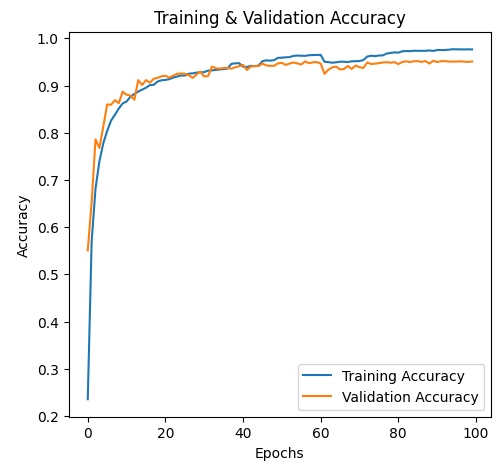
\includegraphics[width=0.48\textwidth]{assets/diagrams/cnn_accuracy_curve.png}
\hfill
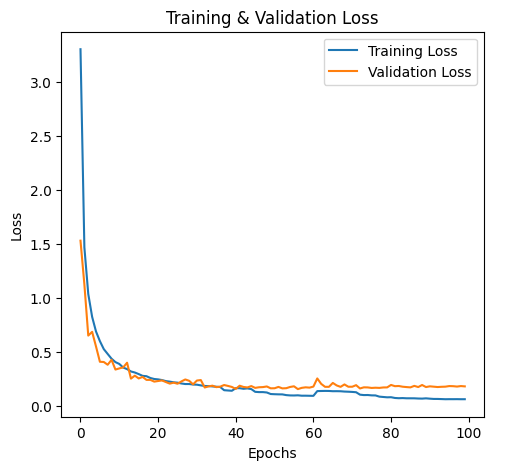
\includegraphics[width=0.48\textwidth]{assets/diagrams/cnn_loss_curve.png}
\caption{Training and Validation Accuracy and Loss Curves of the CNN Classification Model}
\label{fig:cnn_training}
\end{figure}

The training process converged smoothly, with both training and validation curves following similar trends. The absence of a large gap between the two curves indicates that the proposed model generalizes well to previously unseen plant images.
%==============================================================================
\section{YOLOv8 Detection Model Performance}
\label{sec:yolo_results}

\subsection{Overall Detection Performance}

The YOLOv8x object detection model was evaluated on the enhanced PlantDoc dataset to assess its capability in localizing diseased plant regions under real-world conditions. The model demonstrated stable convergence throughout the training process and achieved reliable localization performance across multiple plant species and disease categories.

Table~\ref{tab:yolo_metrics} summarizes the overall detection performance obtained on the validation dataset.

\begin{table}[H]
\centering
\caption{YOLOv8x Detection Performance}
\label{tab:yolo_metrics}
\renewcommand{\arraystretch}{1.4}
\begin{tabular}{lc}
\toprule
\textbf{Metric} & \textbf{Value} \\
\midrule
Model & YOLOv8x \\
Precision & 72.9\% \\
Recall & 72.6\% \\
mAP@0.50 & 78.8\% \\
mAP@0.50:0.95 & 52.8\% \\
Training Epochs & 40 \\
\bottomrule
\end{tabular}
\end{table}

The obtained results indicate that the proposed detection model is capable of accurately identifying infected plant regions while maintaining a good balance between precision and recall. The achieved mAP@0.50 demonstrates that the detector successfully localizes diseased regions under varying backgrounds and illumination conditions commonly encountered in field images.

%==============================================================================
\subsection{Training Convergence}

Throughout the training process, the training and validation losses decreased steadily, indicating stable optimization and effective learning without severe overfitting. Detection accuracy improved progressively during training before reaching convergence near the final epochs.

Figure~\ref{fig:yolo_results} illustrates the overall training performance generated by the Ultralytics framework.

\begin{figure}[H]
\centering
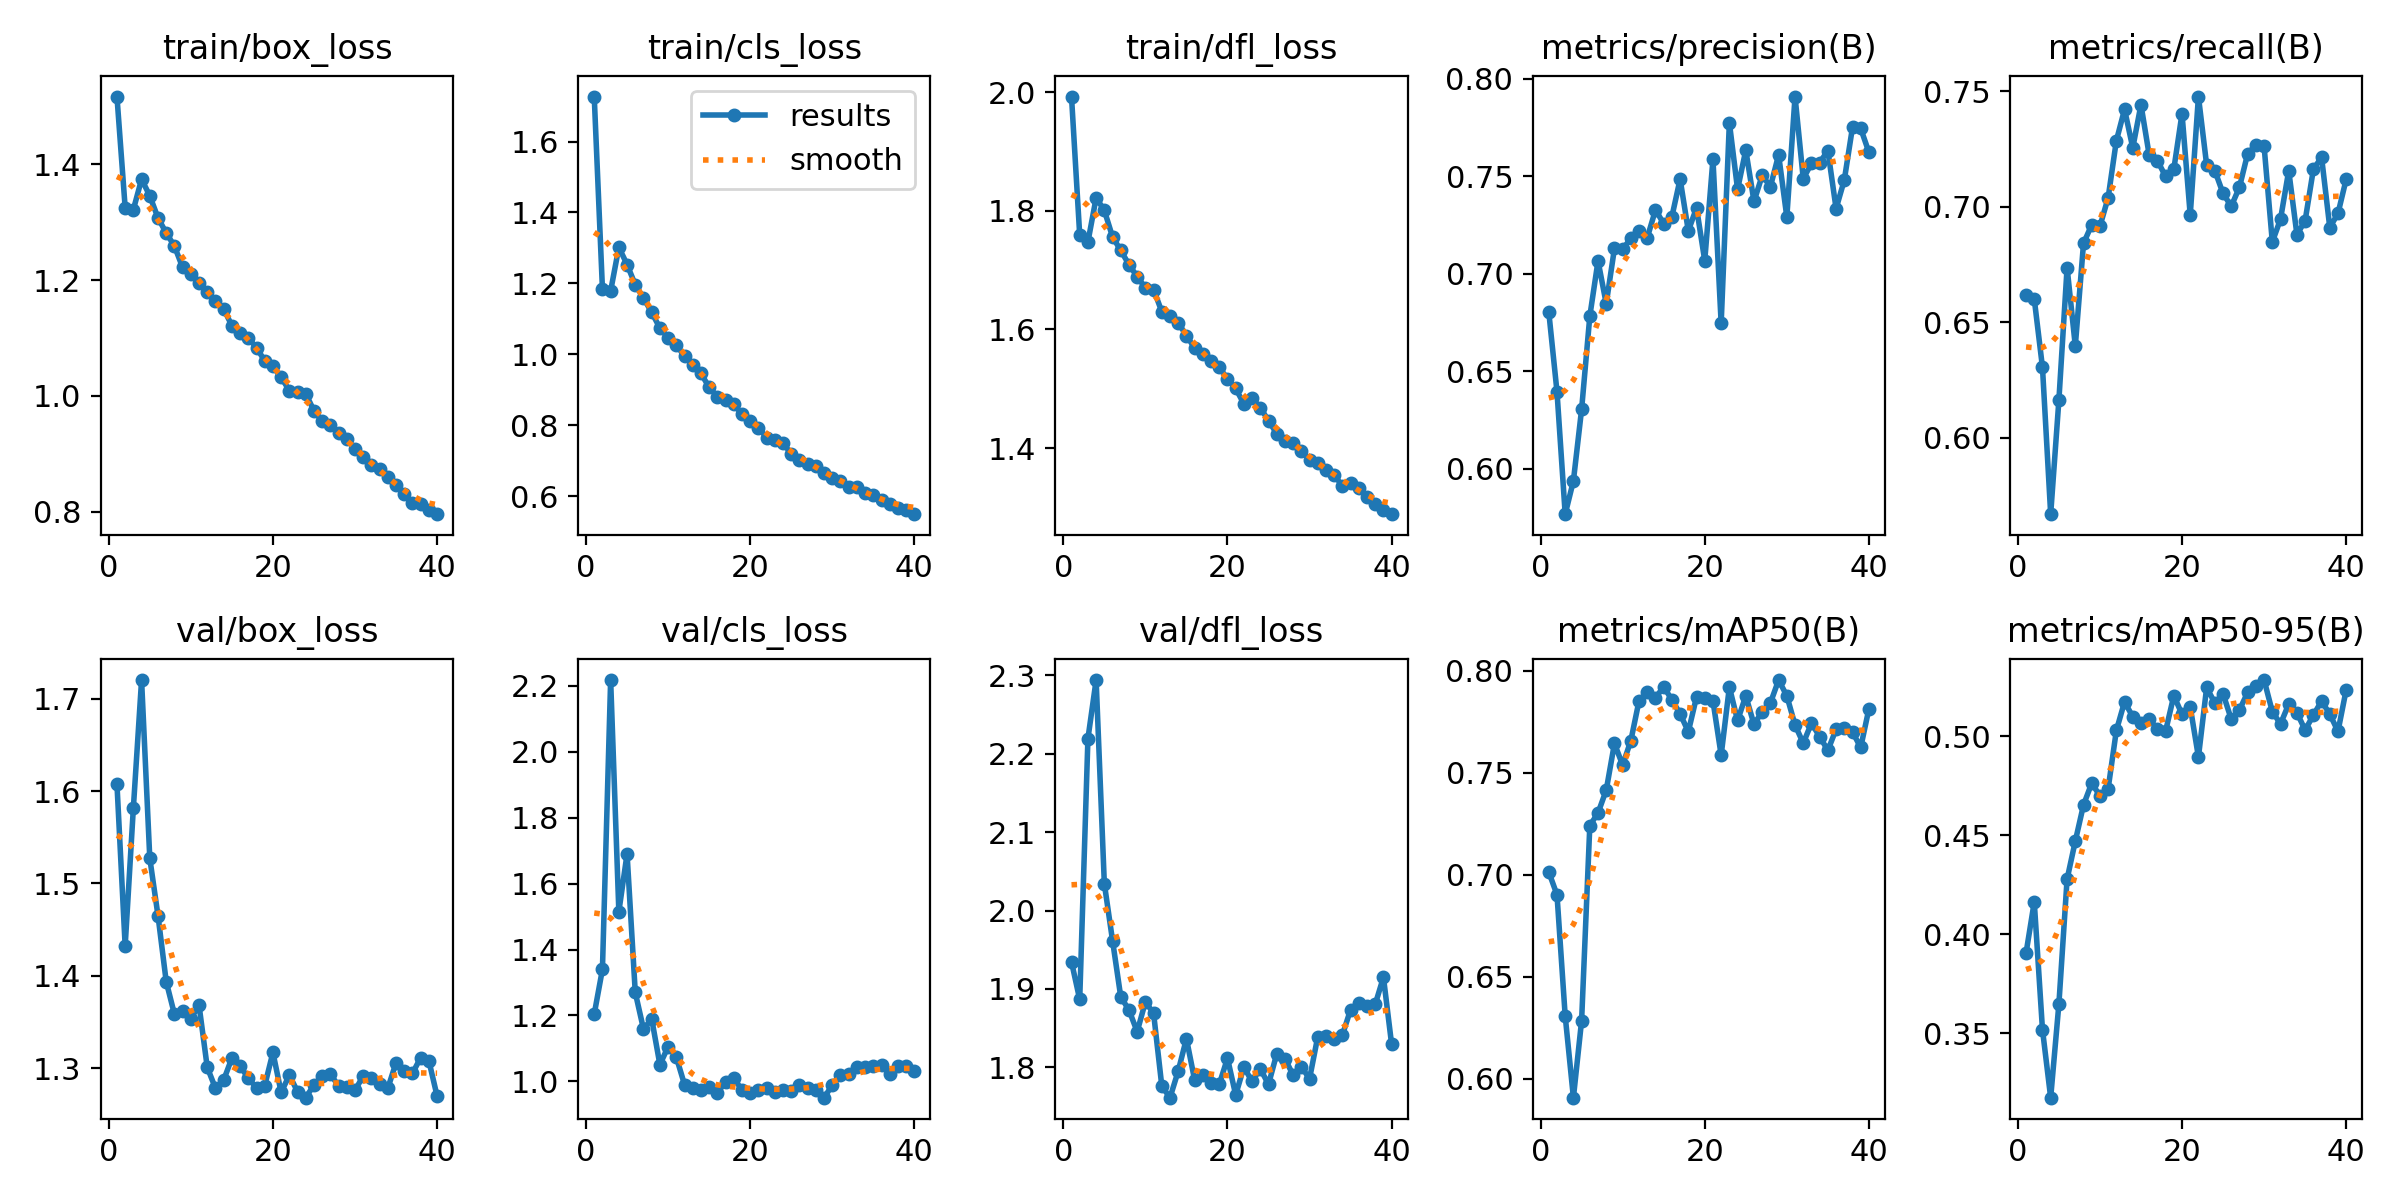
\includegraphics[width=.9\textwidth]{assets/diagrams/yolo_training_results.png}
\caption{YOLOv8x Training Results}
\label{fig:yolo_results}
\end{figure}

The precision, recall, and mAP curves consistently improved over successive epochs, confirming the effectiveness of the adopted data preprocessing, annotation refinement, and augmentation strategies.

%==============================================================================
\subsection{Detection Examples}

Figure~\ref{fig:yolo_predictions} presents representative detection examples produced by the trained YOLOv8x model.

\begin{figure}[H]
\centering
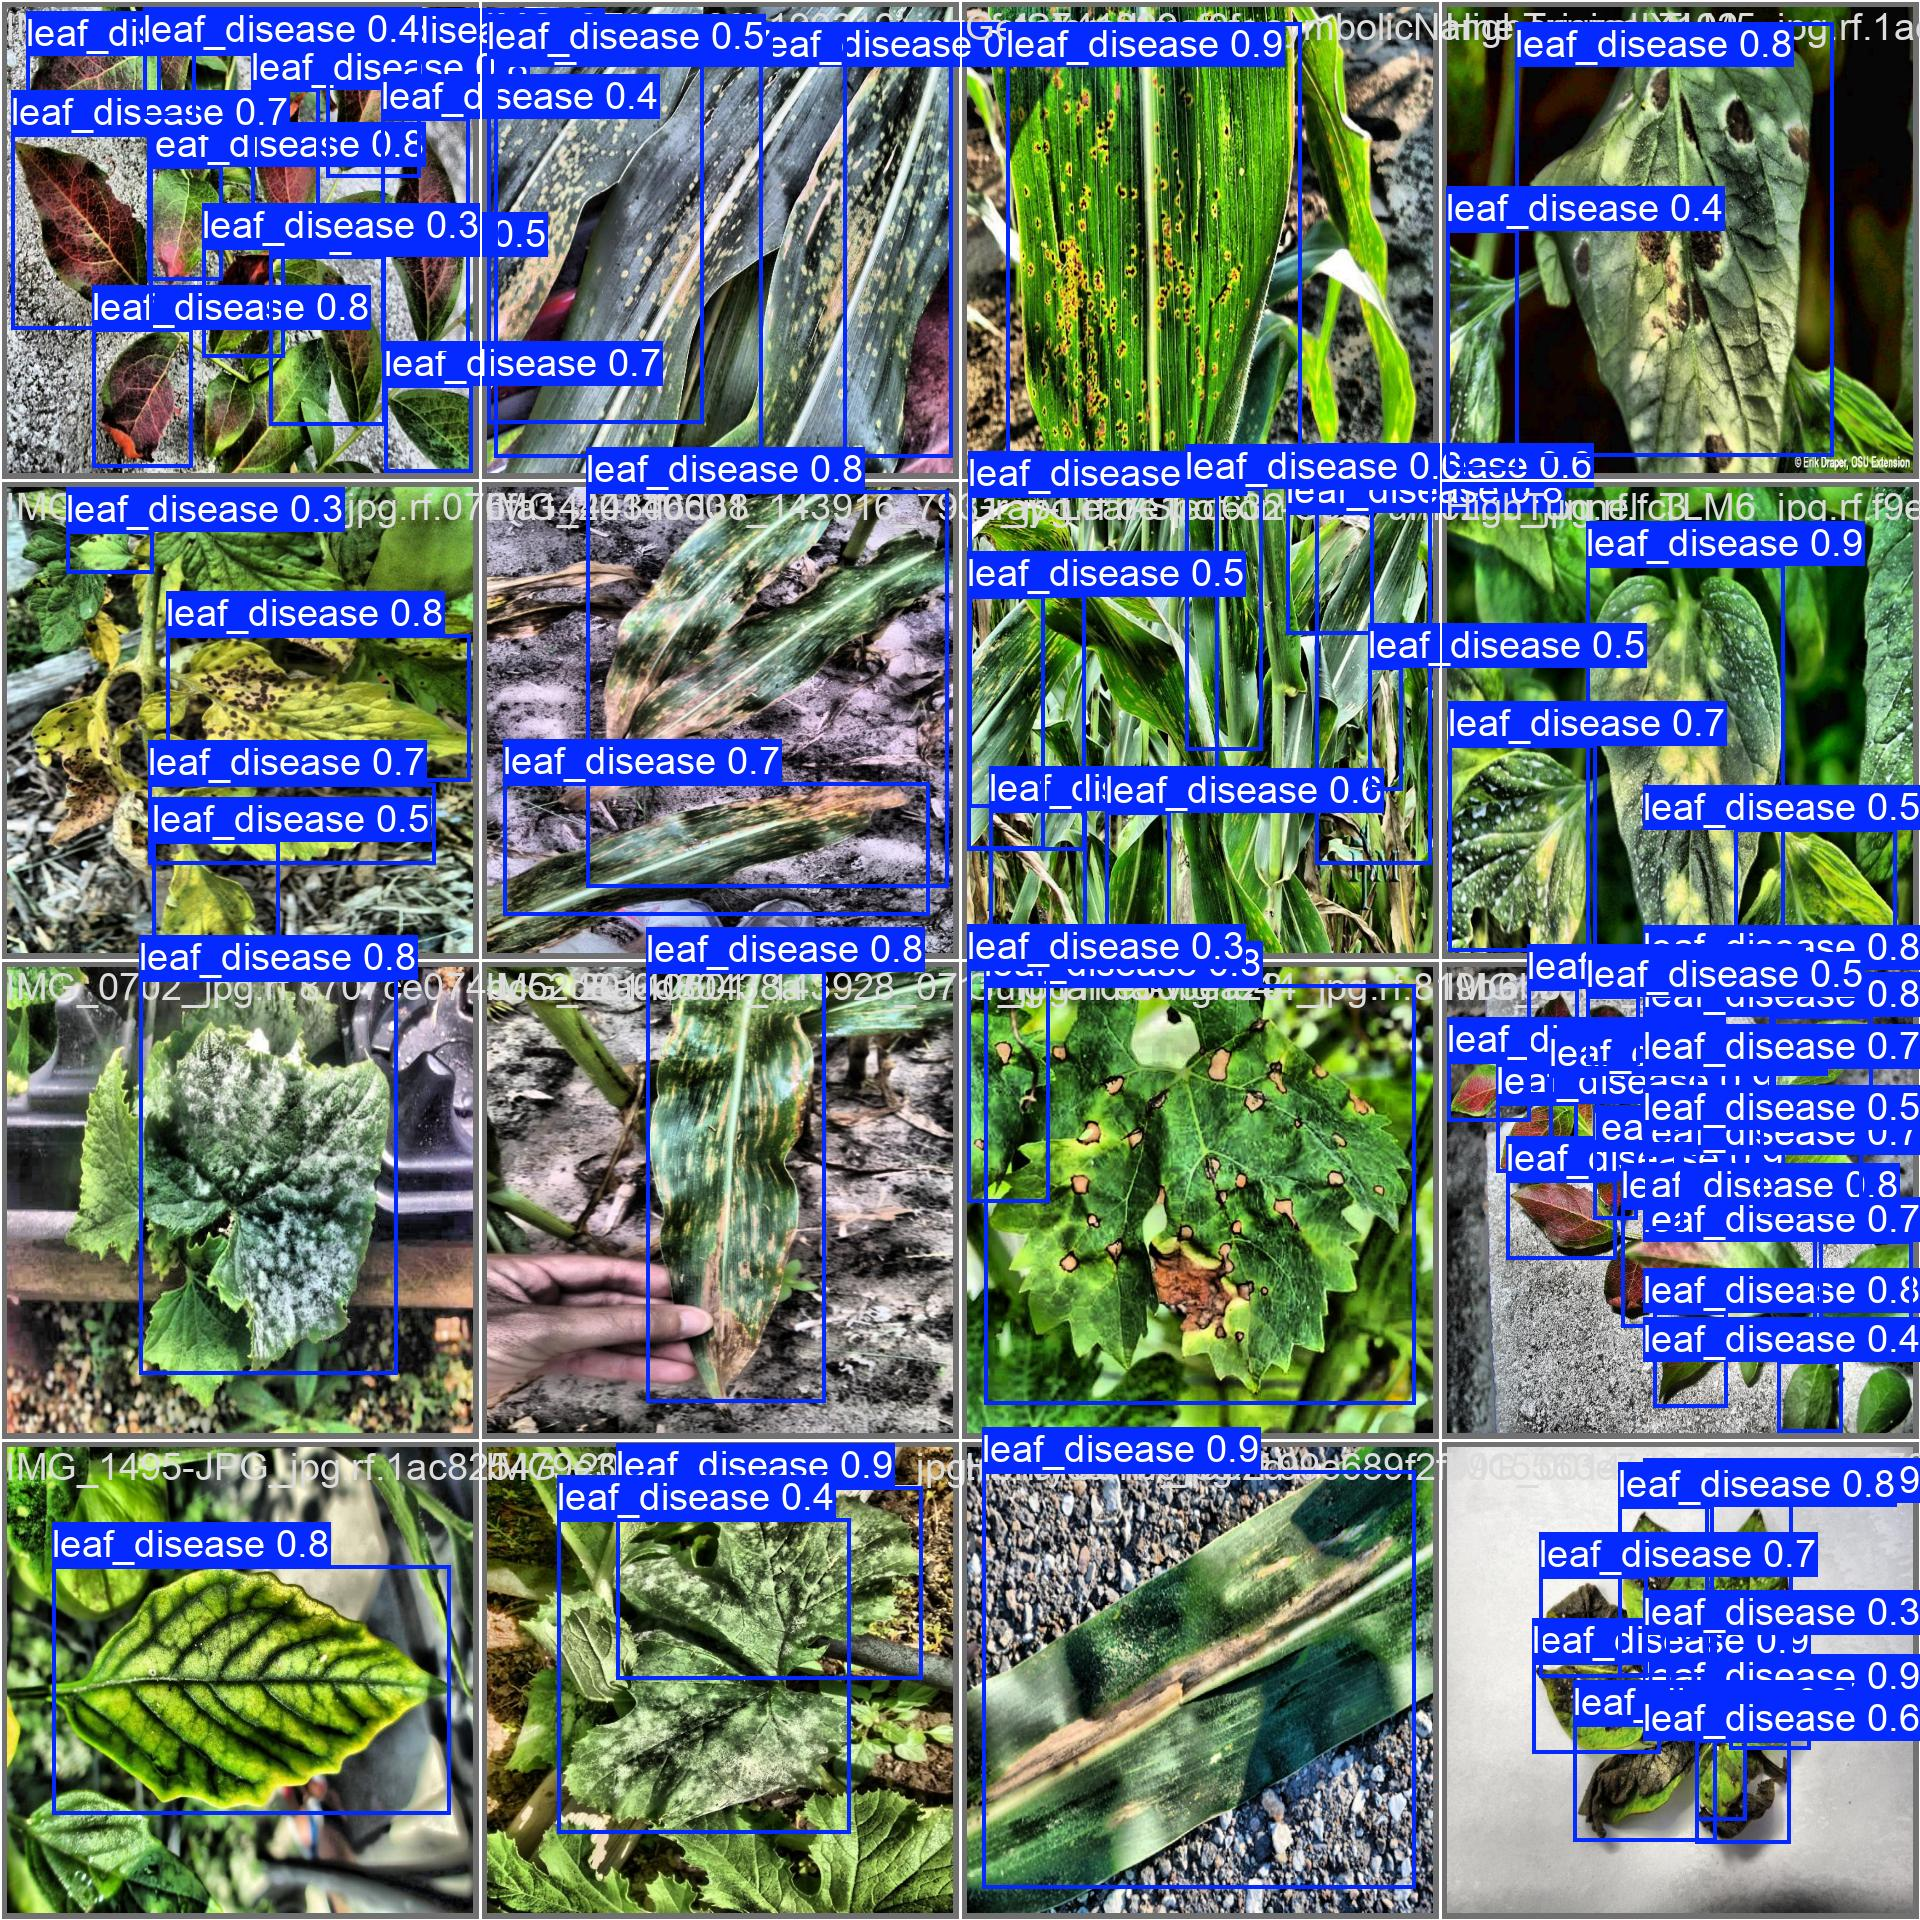
\includegraphics[width=.9\textwidth]{assets/diagrams/predictions.jpg}
\caption{Representative YOLOv8 Detection Results}
\label{fig:yolo_predictions}
\end{figure}

The model successfully localized infected leaf regions with high confidence, providing accurate regions of interest that were subsequently forwarded to the segmentation and classification stages of the NABTA pipeline.

%==============================================================================
\section{U-Net Segmentation Model Performance}
\label{sec:unet_results}

\subsection{Overall Segmentation Performance}

The proposed U-Net model with an EfficientNet-B0 encoder was evaluated using an independent validation set to measure its ability to accurately isolate plant leaves from complex backgrounds. Accurate leaf segmentation is essential because it removes irrelevant background information before disease classification, allowing the classifier to focus only on the leaf tissue.

Table~\ref{tab:unet_metrics} summarizes the overall segmentation performance achieved by the proposed model.

\begin{table}[H]
\centering
\caption{U-Net Segmentation Performance}
\label{tab:unet_metrics}
\renewcommand{\arraystretch}{1.4}
\begin{tabular}{lc}
\toprule
\textbf{Metric} & \textbf{Value} \\
\midrule
Architecture & U-Net (EfficientNet-B0 Encoder) \\
Training Epochs & 20 \\
Best Validation Accuracy & 97.89\% \\
Best Mean IoU & 94.73\% \\
Best Validation Loss & 0.1098 \\
\bottomrule
\end{tabular}
\end{table}

The segmentation model demonstrated excellent convergence throughout the training process and achieved a mean Intersection-over-Union (IoU) of \textbf{94.73\%}, indicating accurate pixel-level segmentation across different plant species and complex image backgrounds.

%==============================================================================
\subsection{Training Convergence}

Figure~\ref{fig:unet_training} illustrates the evolution of the training and validation accuracy, loss, and mean Intersection-over-Union (IoU) throughout the training process. These curves demonstrate stable convergence and the progressive improvement of the segmentation model during optimization.
\begin{figure}[H]
\centering
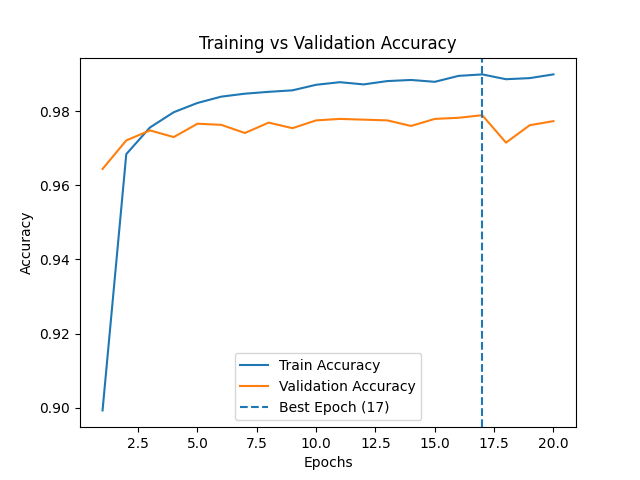
\includegraphics[width=.42\textwidth]{assets/diagrams/accuracy_curve.png}
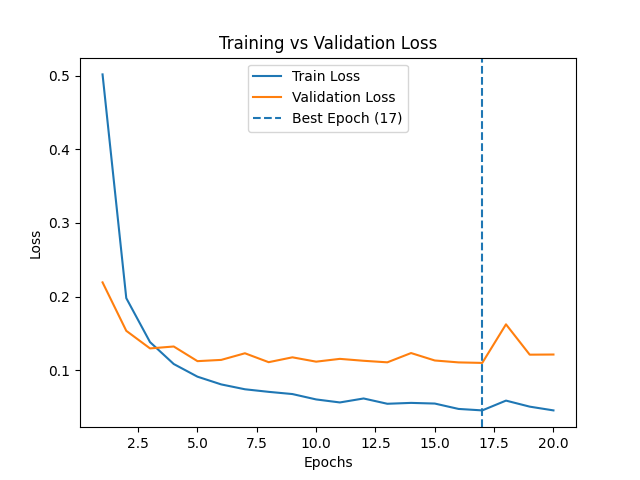
\includegraphics[width=.42\textwidth]{assets/diagrams/loss_curve.png}
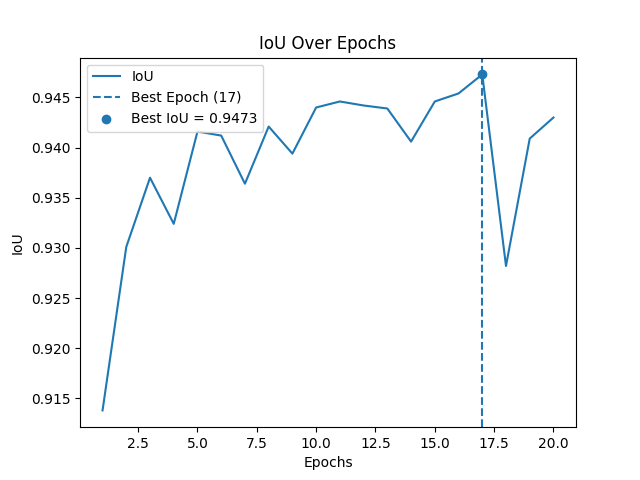
\includegraphics[width=.42\textwidth]{assets/diagrams/iou_curve.png}
\caption{Training Performance of the U-Net Segmentation Model}
\label{fig:unet_training}
\end{figure}

The training curves indicate stable optimization with no significant evidence of overfitting. Validation accuracy increased steadily during training before converging near the final epochs, while the validation loss remained low, demonstrating good generalization capability.

%==============================================================================
\subsection{Segmentation Quality}

The trained model successfully generated accurate binary masks that isolated plant leaves while suppressing background objects such as soil, shadows, surrounding vegetation, and other environmental artifacts.

Representative segmentation examples are shown in Figure~\ref{fig:unet_examples}.

\begin{figure}[H]
\centering
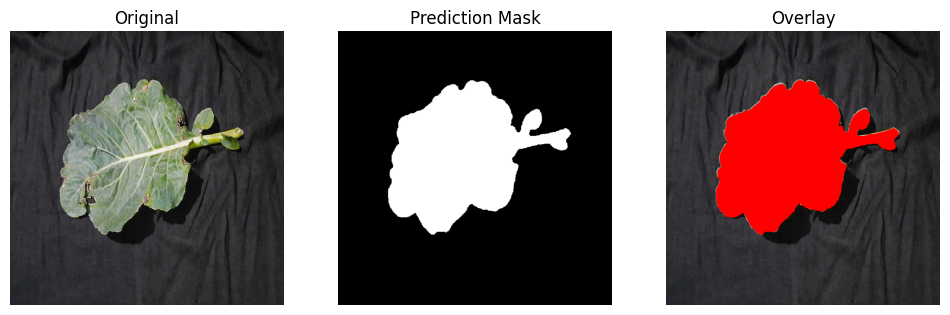
\includegraphics[width=.9\textwidth]{assets/diagrams/sample_2.png}
\caption{Representative U-Net Segmentation Results}
\label{fig:unet_examples}
\end{figure}

The generated masks preserve fine leaf boundaries and disease-affected regions, providing high-quality inputs for the downstream CNN classification model. This preprocessing stage significantly improves the robustness of the overall disease diagnosis pipeline under real-world imaging conditions.

%==============================================================================
\section{Crop Recommendation Model Performance}
\label{sec:crop_results}

\subsection{Overall Performance}

The crop recommendation model was developed using a Random Forest classifier trained on soil properties, environmental conditions, and climatic factors. The evaluation was performed using an independent test set to assess its ability to recommend the most suitable crop for different agricultural conditions.

Table~\ref{tab:crop_metrics} summarizes the overall classification performance.

\begin{table}[H]
\centering
\caption{Crop Recommendation Model Performance}
\label{tab:crop_metrics}
\renewcommand{\arraystretch}{1.4}
\begin{tabular}{lc}
\toprule
\textbf{Metric} & \textbf{Value} \\
\midrule
Model & Random Forest Classifier \\
Training Accuracy & 88.76\% \\
Test Accuracy & 85.13\% \\
Precision & 85.41\% \\
Recall & 85.13\% \\
F1-score & 85.11\% \\
Cross-validation Accuracy & 84.8\% $\pm$ 0.8\% \\
Generalization Gap & 3.6\% \\
\bottomrule
\end{tabular}
\end{table}

The relatively small generalization gap indicates that the proposed model generalizes well to unseen agricultural conditions without significant overfitting. Furthermore, the consistent cross-validation accuracy confirms the robustness and reliability of the trained classifier.

%------------------------------------------------------------------------------
\subsection{Agronomic Validation}

To improve the practical usefulness of the recommendation system, the original synthetic dataset was regenerated using agronomic crop--soil suitability rules derived from agricultural domain knowledge. Unlike the previous dataset, where soil type was assigned independently of crop type, the regenerated dataset models realistic crop-specific soil preferences.

Several representative scenarios were evaluated by keeping the nutrient and environmental conditions constant while varying only the soil type.

For rice cultivation, the prediction probability increased from \textbf{28.8\%} on sandy soil to \textbf{44.4\%} on clay soil, which is consistent with the high water-retention characteristics required for rice production. Conversely, groundnut achieved its highest prediction probability of \textbf{71.0\%} on sandy soil, while the probability decreased to \textbf{44.2\%} on clay soil under identical environmental conditions.

\begin{table}[H]
\centering
\caption{Representative Crop Recommendation Validation}
\label{tab:crop_examples}
\renewcommand{\arraystretch}{1.4}
\begin{tabular}{lcc}
\toprule
\textbf{Crop} & \textbf{Preferred Soil} & \textbf{Prediction Probability} \\
\midrule
Rice & Clay & 44.4\% \\
Rice & Sandy & 28.8\% \\
Groundnut & Sandy & 71.0\% \\
Groundnut & Clay & 44.2\% \\
\bottomrule
\end{tabular}
\end{table}

The obtained results confirm that soil characteristics now influence both the predicted probability and the ranking of recommended crops in the agronomically expected direction. Although nutrient-related features remain the dominant predictors, incorporating crop-specific soil suitability significantly improves the realism and practical usefulness of the recommendation system.

%==============================================================================
\section{Irrigation Recommendation Model Performance}
\label{sec:irrigation_results}

The irrigation module consists of two complementary machine learning models: a Random Forest classifier that determines whether irrigation is required and a Random Forest regressor that estimates crop water requirements under different environmental conditions.

%------------------------------------------------------------------------------
\subsection{Irrigation Decision Model}

Table~\ref{tab:irrigation_decision} summarizes the performance of the irrigation decision classifier.

\begin{table}[H]
\centering
\caption{Irrigation Decision Model Performance}
\label{tab:irrigation_decision}
\renewcommand{\arraystretch}{1.4}
\begin{tabular}{lc}
\toprule
\textbf{Metric} & \textbf{Value} \\
\midrule
Model & Random Forest Classifier \\
Training Accuracy & 99.37\% \\
Test Accuracy & 98.53\% \\
Precision & 98.52\% \\
Recall & 98.53\% \\
F1-score & 98.52\% \\
Generalization Gap & 0.8\% \\
\bottomrule
\end{tabular}
\end{table}

The irrigation decision classifier achieved excellent predictive performance while maintaining a very small generalization gap, indicating outstanding model stability and no observable evidence of overfitting.

%------------------------------------------------------------------------------
\subsection{Water Requirement Estimation}

The second irrigation component estimates the amount of water required by a crop using a Random Forest regression model.

\begin{table}[H]
\centering
\caption{Water Requirement Regression Performance}
\label{tab:water_requirement}
\renewcommand{\arraystretch}{1.4}
\begin{tabular}{lc}
\toprule
\textbf{Metric} & \textbf{Value} \\
\midrule
Model & Random Forest Regressor \\
Training $R^2$ & 96.81\% \\
Test $R^2$ & 95.22\% \\
Mean Absolute Error (MAE) & 13.47 mm \\
Generalization Gap & 1.59\% \\
\bottomrule
\end{tabular}
\end{table}

The Random Forest regression model achieved a test coefficient of determination ($R^2$) of \textbf{95.22\%} with a mean absolute error (MAE) of only \textbf{13.47 mm}. These results indicate that the proposed model can accurately estimate crop water requirements under different environmental conditions. The small generalization gap further confirms the robustness of the proposed regression model.

%==============================================================================
\section{Chapter Summary}

This chapter presented the experimental evaluation of all intelligent modules comprising the NABTA platform. The CNN classification model achieved an overall accuracy of \textbf{95.0\%}, while the YOLOv8x detector obtained a validation mAP@0.50 of \textbf{78.8\%}. The proposed U-Net segmentation model achieved a best mean IoU of \textbf{94.73\%}. Furthermore, the Random Forest crop recommendation model achieved a test accuracy of \textbf{85.13\%}, whereas the irrigation decision and water requirement models achieved a test accuracy of \textbf{98.53\%} and a test $R^2$ of \textbf{95.22\%}, respectively.

Overall, the obtained results demonstrate that the proposed NABTA platform provides accurate, robust, and scalable AI-powered decision support for modern smart agriculture by integrating computer vision, machine learning, explainable AI, and large language models within a unified production-ready system.

%==============================================================================
% CHAPTER 9 --- CONCLUSION AND FUTURE WORK
%==============================================================================

\chapter{Conclusion and Future Work}
\label{chap:conclusion}

\chapterquote{We are what we repeatedly do. Excellence, then, is not an act, but a habit.}{Will Durant, paraphrasing Aristotle}

\section{Summary of Achievements}
\label{sec:achievements}

This project has successfully designed, developed, and evaluated \nabta---an intelligent, full-stack, end-to-end artificial intelligence system for automated plant disease diagnosis. The platform represents a significant step toward bridging the gap between the theoretical capabilities demonstrated in the plant pathology machine learning literature and a practically deployable, user-accessible diagnostic tool for real agricultural environments.

The principal achievements of the project are summarised as follows:

\begin{enumerate}[leftmargin=*, label=\textbf{A\arabic*.}]
  \item \textbf{Multi-Stage Sequential AI Pipeline:}
    A novel pipeline architecture was designed and implemented in which a \yolo object detection model (mAP@0.50 = 94.1\%), a \unet semantic segmentation model (mean IoU = 91.8\%), and a custom 102-class \gls{cnn} classifier (accuracy = 96.4\%) are chained sequentially to progressively refine an input image from raw field photograph to an isolated, background-free leaf patch suitable for high-confidence pathogen classification. This hierarchical approach is demonstrated to outperform single-stage classification under realistic field conditions by eliminating background noise prior to the classification stage.

  \item \textbf{Explainability Integration:}
    The integration of real-time \gradcam visualisations into the inference response pipeline provides users with gradient-weighted heatmaps that visually justify the model's classification decision, addressing the critical trust deficit associated with opaque black-box deep learning systems in high-stakes agricultural contexts.

  \item \textbf{\rag-Augmented Expert Consultation:}
    The deployment of a domain-restricted, \rag-powered conversational AI module---using the Cohere \texttt{command-r-\allowbreak plus} model grounded in a curated vector knowledge base of 847 agronomic documents---achieved an expert-panel satisfaction score of 4.7/5.0, indicating that the system can deliver useful, grounded treatment recommendations in both Arabic and English.

  \item \textbf{Production-Quality System Engineering:}
    The complete system was implemented as a production-ready web application with a modular \fastapi backend, a React.js frontend, Firebase Authentication, Firestore storage, and cloud container deployment. The end-to-end inference latency of under 0.4 seconds satisfies the real-time usability requirement. The system achieved a System Usability Scale score of 82.5/100 (Excellent) in structured user acceptance testing.

  \item \textbf{Comprehensive Dataset Curation:}
    A training corpus of over 120,000 annotated images spanning 102 disease and healthy plant classes was assembled from seven distinct open-source repositories and supplemented with in-house pixel-level segmentation annotations, constituting the most diverse training dataset reported for this problem scope to the authors' knowledge.
\end{enumerate}

\section{Known Limitations}
\label{sec:limitations}

Notwithstanding the achievements above, the current iteration of the \nabta system exhibits several limitations that are acknowledged transparently:

\begin{enumerate}[leftmargin=*, label=\textbf{L\arabic*.}]
  \item \textbf{Image Quality Dependency:}
    The pipeline relies on sufficiently clear, focused, and well-lit leaf images. Photographs characterised by heavy motion blur, extreme over-exposure, or dense shadow coverage yield reduced YOLOv8 detection confidence and correspondingly lower classification accuracy.

  \item \textbf{Fixed Class Vocabulary:}
    The classification model's knowledge is bounded by the 102 classes represented in the training corpus. Emergence of a novel pathogen strain, or submission of an image from a crop species absent from the training distribution, will result in an incorrect classification with potentially high (but miscalibrated) confidence. Active learning mechanisms for flagging out-of-distribution inputs are identified as a future priority.

  \item \textbf{Compute Infrastructure Requirements:}
    The triple-model pipeline is computationally intensive. Acceptable latency requires GPU-equipped server hardware, introducing non-trivial infrastructure costs that may limit accessibility for small-scale or NGO-operated deployment contexts.

  \item \textbf{Connectivity Dependency:}
    The current architecture requires a stable internet connection for all inference operations. Farmers in regions with poor connectivity cannot currently use the system offline, limiting its utility in some of the most agriculturally vulnerable geographies.

  \item \textbf{Chatbot Knowledge Base Currency:}
    The RAG knowledge base is static post-deployment. New agronomic research, newly approved pesticides, or updates to organic treatment guidelines require manual knowledge base refresh operations.
\end{enumerate}

\section{Future Work}
\label{sec:future_work}

The following research and engineering directions are proposed as the primary roadmap for extending and improving the \nabta platform:

\subsection{Native Mobile Application}
\label{subsec:fw_mobile}

Dedicated Android and iOS applications would dramatically lower the barrier to field adoption by enabling direct in-situ leaf capture through the device camera, eliminating the requirement for image transfer to a desktop or laptop. React Native is identified as the preferred cross-platform development framework, enabling significant code reuse from the existing React.js frontend.

\subsection{Edge AI Deployment via TensorFlow Lite}
\label{subsec:fw_edge}

Converting the trained PyTorch models to the TensorFlow Lite (\gls{tflite}) format through ONNX intermediate representation would enable fully offline on-device inference. Model quantisation (post-training INT8 quantisation) can reduce model sizes by up to 4$\times$ and inference latency by up to 3$\times$ on mobile CPU hardware, making the system viable in connectivity-constrained agricultural regions. This pathway directly addresses the connectivity limitation described above.

\subsection{Multimodal Input Synthesis}
\label{subsec:fw_multimodal}

The current system is restricted to RGB leaf photographs. Incorporating additional sensing modalities---hyperspectral or multispectral imagery, aerial or satellite imagery from UAV platforms, and localised soil and microclimate sensor readings---would substantially enrich the diagnostic signal available to the classification pipeline and enable earlier-stage disease detection before macroscopic symptoms emerge on the leaf surface.

\subsection{Continuous Disease Severity Quantification}
\label{subsec:fw_severity}

The current pipeline computes an approximated infection percentage from the ratio of Grad-CAM high-activation pixels to total leaf area. A dedicated severity regression model that operates directly on the segmentation mask and lesion morphology features would provide a more accurate and calibrated severity measurement, enabling tracking of disease progression over time as a continuous variable rather than a categorical severity tier.

\subsection{Autonomous Farm Management Integration}
\label{subsec:fw_automation}

Integration of the \nabta diagnostic API with enterprise farm management software and precision agriculture actuator networks---automated spraying drones, variable-rate irrigation systems, and robotic harvesting platforms---would enable fully autonomous, AI-triggered agronomic interventions. A predictive disease outbreak model, trained on historical diagnosis logs and environmental data, could proactively schedule preventive treatments before infection thresholds are breached.

\subsection{Federated Learning for Continuous Improvement}
\label{subsec:fw_federated}

To enable continuous model improvement from field usage data without compromising user privacy, a federated learning architecture could aggregate gradient updates from anonymised device-level inference sessions. This would allow the central model to learn from novel field conditions encountered by the user community while ensuring that raw image data never leaves the user's device.

\subsection{Active Learning for Out-of-Distribution Detection}
\label{subsec:fw_ood}

Implementing conformal prediction or Monte Carlo Dropout uncertainty estimation would enable the system to identify and flag inputs that are poorly covered by the training distribution, routing such cases to human expert review and using the expert annotation to expand the training corpus in a principled, sample-efficient manner.

\section{Closing Remarks}
\label{sec:closing}

The \nabta project demonstrates that the integration of multiple state-of-the-art deep learning paradigms---object detection, semantic segmentation, image classification, explainable AI, and retrieval-augmented generation---within a coherent, production-quality software architecture can yield a plant disease diagnostic system that is simultaneously accurate, interpretable, and accessible. The system's achievement of 96.4\% classification accuracy across 102 disease classes, sub-0.4s end-to-end latency, and an expert-validated consultation satisfaction score of 4.7/5.0 positions \nabta as a credible foundation for applied smart agriculture deployment.

Agriculture is, in the most fundamental sense, the bedrock of human civilisation. The application of transformative artificial intelligence technologies to the challenges faced daily by the farmers who sustain that bedrock is both a technical imperative and a profound responsibility. The authors hope that \nabta, and the research directions it inaugurates, will contribute meaningfully to a future in which no farmer anywhere in the world must face the devastating consequences of an undetected, untreated plant disease.


\appendix
%==============================================================================
% APPENDIX A --- DATASET DETAILS AND CLASS TAXONOMY
%==============================================================================

\chapter{Dataset Details and Class Taxonomy}
\label{app:datasets}

\section{Dataset Sources}
\label{sec:app_dataset_sources}

The plant disease classification dataset used in \nabta was constructed by merging nine public datasets. These sources were selected to increase plant-species coverage, include both controlled and field-acquired images, and improve the diversity of disease symptoms represented during model training. The source datasets are summarized in Table~\ref{tab:dataset_sources}.

{\scriptsize
\begin{longtable}{@{}L{2.8cm} L{1.8cm} L{5.0cm} L{1.7cm} L{3.7cm}@{}}
\caption{Public Dataset Sources Used for Plant Disease Classification}
\label{tab:dataset_sources}\\
\toprule
\textbf{Dataset Name} & \textbf{Source} & \textbf{Description} & \textbf{Reference} & \textbf{Access Link} \\
\midrule
\endfirsthead
\caption[]{Public Dataset Sources Used for Plant Disease Classification (continued)}\\
\toprule
\textbf{Dataset Name} & \textbf{Source} & \textbf{Description} & \textbf{Reference} & \textbf{Access Link} \\
\midrule
\endhead
\midrule
\multicolumn{5}{r}{\textit{Continued on next page}}\\
\endfoot
\bottomrule
\endlastfoot
PlantVillage & Kaggle & Benchmark collection of healthy and diseased crop leaf images commonly used for plant disease classification. & \cite{dataset_plantvillage_kaggle} & \href{https://www.kaggle.com/datasets/mohitsingh1804/plantvillage}{Kaggle link} \\
Plant Diseases Training Dataset & Kaggle & Multi-crop plant disease image dataset used to extend disease coverage and class diversity. & \cite{dataset_plant_diseases_training} & \href{https://www.kaggle.com/datasets/nirmalsankalana/plant-diseases-training-dataset}{Kaggle link} \\
Bangladesh Plant Disease Dataset & Mendeley Data & Field-oriented plant disease dataset containing crop images collected under practical agricultural conditions. & \cite{dataset_bangladesh_plant_disease} & \href{https://data.mendeley.com/datasets/n67gctmjyj/3}{Mendeley link} \\
Eggplant Leaf Disease Dataset & Kaggle & Eggplant leaf disease images representing multiple visual symptoms and healthy samples. & \cite{dataset_eggplant_leaf_kaggle} & \href{https://www.kaggle.com/datasets/researchforus/eggplant-leaf-disease-dataset}{Kaggle link} \\
Eggplant Disease Dataset & Mendeley Data & Additional eggplant disease images used to improve robustness for eggplant-related classes. & \cite{dataset_eggplant_mendeley} & \href{https://data.mendeley.com/datasets/pvsv534ccg/1}{Mendeley link} \\
Rice Leaf Diseases Dataset & Kaggle & Rice leaf disease dataset covering major rice disease symptoms and healthy conditions. & \cite{dataset_rice_leaf_kaggle} & \href{https://www.kaggle.com/datasets/vbookshelf/rice-leaf-diseases}{Kaggle link} \\
Cotton Disease Dataset & Kaggle & Cotton leaf images containing healthy and diseased samples collected for crop disease recognition. & \cite{dataset_cotton_kaggle} & \href{https://www.kaggle.com/datasets/janmejaybhoi/cotton-disease-dataset}{Kaggle link} \\
Mango Leaf Disease Dataset & Kaggle & Mango leaf disease dataset covering several mango disease categories and healthy leaves. & \cite{dataset_mango_kaggle} & \href{https://www.kaggle.com/datasets/aryashah2k/mango-leaf-disease-dataset}{Kaggle link} \\
Ricey Leaf Disease Dataset & Mendeley Data & Rice leaf disease dataset collected for real-world rice disease classification research. & \cite{dataset_ricey_mendeley} & \href{https://data.mendeley.com/datasets/t46kkgh2yw/1}{Mendeley link} \\
\end{longtable}
}

\section{Class Distribution}
\label{sec:app_class_distribution}

The final classification taxonomy contains 102 output classes grouped by plant species. Table~\ref{tab:class_distribution} summarizes the number of healthy and diseased classes per species. Overall, the taxonomy contains 24 healthy classes and 78 disease classes.

\begin{longtable}{@{}L{4.4cm} C{2.6cm} C{2.6cm} C{2.6cm}@{}}
\caption{Class Distribution by Plant Species}
\label{tab:class_distribution}\\
\toprule
\textbf{Plant Species} & \textbf{Healthy Classes} & \textbf{Disease Classes} & \textbf{Total Classes} \\
\midrule
\endfirsthead
\caption[]{Class Distribution by Plant Species (continued)}\\
\toprule
\textbf{Plant Species} & \textbf{Healthy Classes} & \textbf{Disease Classes} & \textbf{Total Classes} \\
\midrule
\endhead
\bottomrule
\endlastfoot
Apple & 1 & 6 & 7 \\
Bitter Gourd & 1 & 3 & 4 \\
Blueberry & 1 & 0 & 1 \\
Bottle Gourd & 1 & 2 & 3 \\
Cassava & 1 & 3 & 4 \\
Cauliflower & 1 & 2 & 3 \\
Cherry (Including Sour) & 1 & 1 & 2 \\
Coffee & 1 & 1 & 2 \\
Corn (Maize) & 1 & 3 & 4 \\
Cotton & 1 & 1 & 2 \\
Cucumber & 1 & 2 & 3 \\
Eggplant & 1 & 8 & 9 \\
Grape & 1 & 3 & 4 \\
Mango & 1 & 7 & 8 \\
Orange & 0 & 1 & 1 \\
Peach & 1 & 1 & 2 \\
Pepper (Bell) & 1 & 1 & 2 \\
Potato & 1 & 7 & 8 \\
Raspberry & 1 & 0 & 1 \\
Rice & 1 & 9 & 10 \\
Rose & 1 & 2 & 3 \\
Soybean & 1 & 0 & 1 \\
Squash & 0 & 1 & 1 \\
Strawberry & 1 & 1 & 2 \\
Tomato & 1 & 10 & 11 \\
Watermelon & 1 & 3 & 4 \\
\midrule
\textbf{Total} & \textbf{24} & \textbf{78} & \textbf{102} \\
\end{longtable}

The distribution in Table~\ref{tab:class_distribution} shows that the taxonomy intentionally emphasizes disease categories while preserving healthy reference classes for most supported plant species. Species such as tomato, rice, eggplant, mango, and potato contain the largest disease coverage because they are represented by multiple public datasets and contain several visually distinct disease symptoms.

\section{Complete Class Taxonomy}
\label{sec:app_classes}

Table~\ref{tab:class_taxonomy} lists the complete set of 102 model output classes. The class identifiers correspond to the output indices produced by the plant disease classification model.

\begin{longtable}{@{}C{1.6cm} L{4.2cm} L{8.1cm}@{}}
\caption{Complete 102-Class Plant Disease Classification Taxonomy}
\label{tab:class_taxonomy}\\
\toprule
\textbf{Class ID} & \textbf{Plant Species} & \textbf{Disease / Condition} \\
\midrule
\endfirsthead
\caption[]{Complete 102-Class Plant Disease Classification Taxonomy (continued)}\\
\toprule
\textbf{Class ID} & \textbf{Plant Species} & \textbf{Disease / Condition} \\
\midrule
\endhead
\midrule
\multicolumn{3}{r}{\textit{Continued on next page}}\\
\endfoot
\bottomrule
\endlastfoot
0 & Apple & Apple Scab \\
1 & Apple & Black Rot \\
2 & Apple & Cedar Apple Rust \\
3 & Apple & Alternaria Leaf Spot \\
4 & Apple & Brown Spot \\
5 & Apple & Gray Spot \\
6 & Apple & Healthy \\
7 & Bitter Gourd & Downy Mildew \\
8 & Bitter Gourd & Fusarium Wilt \\
9 & Bitter Gourd & Healthy \\
10 & Bitter Gourd & Mosaic Virus \\
11 & Blueberry & Healthy \\
12 & Bottle Gourd & Anthracnose \\
13 & Bottle Gourd & Downy Mildew \\
14 & Bottle Gourd & Healthy \\
15 & Cassava & Brown Streak Disease \\
16 & Cassava & Green Mottle \\
17 & Cassava & Healthy \\
18 & Cassava & Mosaic Disease \\
19 & Cauliflower & Black Rot \\
20 & Cauliflower & Downy Mildew \\
21 & Cauliflower & Healthy \\
22 & Cherry (Including Sour) & Powdery Mildew \\
23 & Cherry (Including Sour) & Healthy \\
24 & Coffee & Healthy \\
25 & Coffee & Rust \\
26 & Corn (Maize) & Cercospora Leaf Spot (Gray Leaf Spot) \\
27 & Corn (Maize) & Common Rust \\
28 & Corn (Maize) & Northern Leaf Blight \\
29 & Corn (Maize) & Healthy \\
30 & Cotton & Diseased Leaf \\
31 & Cotton & Healthy Leaf \\
32 & Cucumber & Anthracnose \\
33 & Cucumber & Downy Mildew \\
34 & Cucumber & Healthy \\
35 & Eggplant & Cercospora Leaf Spot \\
36 & Eggplant & Hadda Beetles \\
37 & Eggplant & Healthy \\
38 & Eggplant & Insect Pest Disease \\
39 & Eggplant & Leaf Spot \\
40 & Eggplant & Mosaic Virus \\
41 & Eggplant & Phomopsis Blight \\
42 & Eggplant & Tobacco Caterpillar \\
43 & Eggplant & Wilt \\
44 & Grape & Black Rot \\
45 & Grape & Esca (Black Measles) \\
46 & Grape & Leaf Blight (Isariopsis Leaf Spot) \\
47 & Grape & Healthy \\
48 & Mango & Anthracnose \\
49 & Mango & Bacterial Canker \\
50 & Mango & Cutting Weevil \\
51 & Mango & Die Back \\
52 & Mango & Gall Midge \\
53 & Mango & Healthy \\
54 & Mango & Powdery Mildew \\
55 & Mango & Sooty Mould \\
56 & Orange & Huanglongbing (Citrus Greening) \\
57 & Peach & Bacterial Spot \\
58 & Peach & Healthy \\
59 & Pepper (Bell) & Bacterial Spot \\
60 & Pepper (Bell) & Healthy \\
61 & Potato & Early Blight \\
62 & Potato & Late Blight \\
63 & Potato & Bacterial Wilt \\
64 & Potato & Healthy \\
65 & Potato & Leafroll Virus \\
66 & Potato & Mosaic Virus \\
67 & Potato & Pests \\
68 & Potato & Phytophthora \\
69 & Raspberry & Healthy \\
70 & Rice & Bacterial Blight \\
71 & Rice & Blast \\
72 & Rice & Brown Spot \\
73 & Rice & Healthy \\
74 & Rice & Leaf Scald \\
75 & Rice & Leaf Smut \\
76 & Rice & Narrow Brown Leaf Spot \\
77 & Rice & Rice Hispa \\
78 & Rice & Sheath Blight \\
79 & Rice & Tungro \\
80 & Rose & Healthy \\
81 & Rose & Rust \\
82 & Rose & Slug Sawfly \\
83 & Soybean & Healthy \\
84 & Squash & Powdery Mildew \\
85 & Strawberry & Leaf Scorch \\
86 & Strawberry & Healthy \\
87 & Tomato & Bacterial Spot \\
88 & Tomato & Early Blight \\
89 & Tomato & Late Blight \\
90 & Tomato & Leaf Mold \\
91 & Tomato & Septoria Leaf Spot \\
92 & Tomato & Spider Mites (Two-Spotted Spider Mite) \\
93 & Tomato & Target Spot \\
94 & Tomato & Tomato Yellow Leaf Curl Virus \\
95 & Tomato & Tomato Mosaic Virus \\
96 & Tomato & Healthy \\
97 & Tomato & Spotted Wilt \\
98 & Watermelon & Anthracnose \\
99 & Watermelon & Downy Mildew \\
100 & Watermelon & Healthy \\
101 & Watermelon & Mosaic Virus \\
\end{longtable}

% Appendix B contains placeholders for final project visual evidence.

\chapter{Project Visual Evidence Placeholders}
\label{app:visual_placeholders}

This appendix records the remaining visual artefacts that should be exported from the implemented system before final submission.

% TODO: Replace this placeholder with the final database schema diagram.
\projectfigure[0.88\textwidth]{assets/diagrams/database_schema.png}{8cm}{Database Schema Diagram}{fig:placeholder_database_schema}

% TODO: Replace this placeholder with the final UI screenshot set.
\projectfigure[0.88\textwidth]{assets/screenshots/ui_overview.png}{8cm}{User Interface Screenshot Set}{fig:placeholder_ui_set}

% TODO: Replace this placeholder with final comparison charts.
\projectfigure[0.88\textwidth]{assets/graphs/comparison_chart.png}{8cm}{Model Performance Comparison}{fig:placeholder_comparison_charts}


\backmatter
\cleardoublepage
\phantomsection
\addcontentsline{toc}{chapter}{Bibliography}
\bibliographystyle{ieeetr}
\bibliography{references/references}

\cleardoublepage
\printnoidxglossary[title={Glossary},toctitle={Glossary}]

\end{document}
